
% !TEX program = xelatex
\documentclass[11pt,openany]{book}
\usepackage{fontspec}
\setmainfont{Times New Roman}
\setsansfont{Arial}
\setmonofont{Consolas}
\usepackage[paperwidth=185mm,paperheight=260mm,top=23mm,bottom=24mm,inner=22mm,outer=19mm,headsep=6mm,footskip=10mm]{geometry}
\usepackage{amsmath,unicode-math}
\setmathfont{texgyretermes-math.otf}
\usepackage{graphicx,booktabs,tabularx,array,enumitem,xcolor,tikz}
\usetikzlibrary{arrows.meta,positioning,calc,backgrounds,fit}
\usepackage{fancyhdr,ragged2e,caption}
\usepackage{xurl}
\usepackage[hidelinks,unicode]{hyperref}
\usepackage[backend=biber,style=numeric,sorting=none,maxbibnames=5]{biblatex}
\addbibresource{refs.bib}
\AtEveryBibitem{\clearfield{note}}
\definecolor{ink}{HTML}{1A1A1A}
\definecolor{slate}{HTML}{4A5568}
\definecolor{deepblue}{HTML}{2C5282}
\definecolor{terra}{HTML}{8B5E3C}
\definecolor{forest}{HTML}{2F6F4E}
\definecolor{rust}{HTML}{9C4221}
\linespread{1.16}
\setlength{\parindent}{1.25em}
\setlength{\parskip}{0pt}
\setlength{\emergencystretch}{2em}
\newcolumntype{Y}{>{\RaggedRight\arraybackslash}X}
\raggedbottom
\let\cleardoublepage\clearpage
\newcommand{\key}[1]{\textbf{#1}}
\newcommand{\term}[1]{\textbf{#1}}
\newcommand{\subhead}[1]{\par\medskip\noindent\textbf{#1}\par\nobreak\smallskip}
\newcommand{\furtherreading}[1]{\par\medskip\noindent\textbf{Further reading}\par\smallskip{\small\raggedright #1\par}}
\captionsetup{font=small,labelfont=bf,labelsep=quad}
\fancypagestyle{plain}{\fancyhf{}\fancyfoot[C]{\small\thepage}\renewcommand{\headrulewidth}{0pt}}
\pagestyle{fancy}
\fancyhf{}
\fancyhead[LE]{\small\itshape Viscosity}
\fancyhead[RO]{\small\itshape\leftmark}
\fancyfoot[C]{\small\thepage}
\renewcommand{\chaptermark}[1]{\markboth{Chapter \thechapter}{}}
\renewcommand{\topfraction}{0.9}
\renewcommand{\textfraction}{0.08}
\renewcommand{\floatpagefraction}{0.95}
\renewcommand*{\bibfont}{\small\emergencystretch=3em}
\AtBeginBibliography{\RaggedRight}
\setcounter{biburllcpenalty}{3000}
\setcounter{biburlucpenalty}{4000}
\setcounter{biburlnumpenalty}{3000}
\hypersetup{pdftitle={Viscosity: Intelligence Across Bits, Atoms, and Life},pdfsubject={English revised edition}}
\begin{document}
\begin{titlepage}
\centering
\vspace*{32mm}
{\fontsize{42}{46}\selectfont\bfseries Viscosity\par}
\vspace{9mm}
{\Large Intelligence Across Bits, Atoms, and Life\par}
\vspace{14mm}
{\color{rust}\rule{50mm}{0.8pt}\par}
\vspace{13mm}
{\large\itshape The world does not run at inference speed.\par}
\vfill
{\small English edition\\28 October 2026\par}
\vspace*{13mm}
\end{titlepage}
\frontmatter
\chapter*{Preface}
\addcontentsline{toc}{chapter}{Preface}
\markboth{Preface}{Preface}

AI can draft ten proposals before the meeting ends. The organization still has to build, test, and stand behind them. Arguments about artificial intelligence often skip this distance. Optimists expect stronger models and lower costs. Skeptics point to the gap between a demonstration and a working system. Both have evidence. Both often accept the same premise: once intelligence becomes abundant and cheap, the remaining problems will yield. This book starts with that premise.

Generating a plan has become much cheaper. A coherent proposal can arrive in seconds. Turning it into a working production line can still take months or years. Equipment must be ordered, workers trained, processes approved, and responsibility assigned. Advances in model design, training, data, and inference change the first part of this chain much faster than the rest. The bottleneck moves. Confuse cheaper generation with cheaper accomplishment, and every judgment downstream inherits the error.

The first assumption is that intelligence can be measured on a single axis. Its engineering origins are understandable: for a time, larger models, more data, and more computation advanced together with benchmark performance. Extrapolation became a habit. But recognition, reasoning, memory, planning, dexterity, empathy, and responsibility are different capacities, with different enabling conditions. More text does not by itself equip a system to manipulate objects, honor a long commitment, or bear the consequences of an intervention. A stronger score on one axis cannot establish readiness on all the others.

The second assumption extends cheap copying to execution. Digitization has displaced maps, film, records, and many transactions at a counter. Yet copying a bridge design consumes different resources from building a bridge. Distribute the plans ten thousand times; each bridge still needs a site, materials, construction, and inspection. Concrete gains strength under particular mix and curing conditions; the familiar 28-day strength is a testing benchmark. A drug candidate can be generated quickly, while efficacy and long-term safety require experiments and observation. Better design and testing tools improve these processes. Each process still has conditions that must actually be met.

The third assumption is that the better solution will win. Engineering history offers ample reason to doubt it. A technically superior design can lose to an established supply chain, a large installed base, or a cheaper transition. Deployment passes through resource constraints, process time, and inherited dependencies. Optimization may improve only a small part of that passage.

A related misconception concerns people. The usual question is whether machines will replace workers or liberate them. A subtler change can precede either outcome: the connection between a person's abilities and the evidence of their value begins to fail. Writing, calculation, and synthesis once made training and competence visible. When comparable outputs become available on demand, the abilities may remain while their evidential force weakens. Chapters 5 and 6 examine the resulting loss of position and the conditions for rebuilding it.

These assumptions survive because they work well within a restricted setting. Copies are cheap, search is effective, and performance can improve rapidly within a defined task. The mistake arrives when those properties are extended across the boundary of the setting. To locate that boundary, we need to ask where intelligence comes from, what it does, and what changes when it enters material and living systems. Physics, biology, information theory, and engineering supply parts of the answer. This book brings those parts into the same account.

The connecting concept is \term{viscosity}: the cost and resistance involved in moving a system from one state to another. Duration is only one part of it. What resources does the transition consume? What dependencies does it disturb? What remains afterward? What would reversal require? Navigation, digital payments, industrial simulation, automated experiments, and coding tools have reduced such costs in specific places. The useful question is where the reduction occurs, whether total cost falls, and where any remaining burden goes.

Three coordinates organize the analysis. \term{Resource barriers} ($R$) comprise the materials, energy, equipment, and capital needed to produce a change. \term{Temporal rigidity} ($T$) describes the time required for reaction, growth, testing, and coordination. \term{Topological coupling} ($G$) describes the dependencies through which a local change must propagate, including the difficulty of synchronization, isolation, and rollback. An engineering improvement may buy time with resources, reduce several costs together, or shift work into maintenance and verification. Both the total and its distribution matter.

The same constraints behave differently in three media. In \term{bits}, generation, copying, transmission, and revision can be cheap. Verification and trust can remain expensive. In \term{atoms}, manufacturing, construction, transport, energy, and infrastructure confront mass, strength, friction, space, and maintenance. A mistaken sentence can be rewritten; a mistaken movement can break a component or injure a person. In \term{life}, an intervention meets a system that detects, compensates, adapts, and sometimes rebounds. A DNA sequence can be represented as text, but its function depends on the living organization in which it operates. Bits support diffusion, atoms require work, and life responds through feedback. Acceleration takes a different form in each.

The book has seven chapters and an appendix. Chapter 1 examines the mismatch between the speed of generation and the speed of change, then asks how resistance can also stabilize a system. Chapter 2 develops the physical account: the origins of intelligence, the costs of material transformation, and the $R$-$T$-$G$ framework. Computation can improve a route without removing the energy differences along it. Faster search and faster execution are separate achievements.

Chapter 3 follows intelligence across the interface. How do different media absorb its input? When does an overloaded system reroute, accumulate a backlog, or become unstable? Under what conditions can a generated result be treated as established? Chapter 4 carries these questions into organisms, bodies, and mobility. It examines why biological intervention differs from editing software, why a machine cannot simply inherit a biological body's abilities, and why exploration, control, and verification may demand different forms of intelligence. The same account then follows costs through vehicles, infrastructure, and the institutions that govern their use. The practical objective is a viable operating regime for systems whose parts run on different clocks.

Chapter 5 is the center of the book. What qualifies as something we can rely on? When may a representation become an action? Where do the consequences return, and what must a person or organization be able to bear before it can accept responsibility? These questions establish the terms for examining three losses: functional relevance, contact with reality, and agency. At this point, the question of what can be generated becomes inseparable from the question of what can be borne.

Chapter 6 follows the migration of value. Writing, printing, clocks, steam power, and computers each changed how human ability was recognized. As symbolic generation becomes cheaper, verification, care, durable commitments, and responsibility may become scarcer. Their scarcity alone does not secure pay, recognition, or rights; institutions determine those outcomes. Four principles organize the chapter: damping, incompleteness, symbiosis, and recursive improvement. They address how consequences establish a boundary, what objective functions leave out, how complementary roles can be organized, and why change must be evaluated at successive levels. Their practical form is closer to constitutional rules than to a technical specification.

Chapter 7 returns to action: how individuals retain contact with resistance, how organizations rebuild verification and trust, why civilization continues to need demanding frontiers, and how self-replicating systems test the argument. The appendix sets out the generalized-viscosity model, its relation to existing work, and a route from conceptual framework to testable claims.

The sequence matters. The first three chapters establish constraints; the fourth follows their consequences in bodies and motion; the fifth and sixth examine the vacancies left when familiar constraints are bypassed; the seventh returns to choices. Later arguments use premises established earlier. Reading in order makes those dependencies visible.

Constraint analysis connects the engineering and ethical arguments. Idle waiting and redundant work should be removed. Execution and verification should become cheaper. Where an existing arrangement supplies safety, trust, or accountability, an improved arrangement must continue to supply those functions. Physical models help identify the relations involved. Deployment decisions also require task evidence, organizational judgment, and the participation of people who will bear the consequences.

If AI can produce more of what people once produced, what secures a person's place? Ability is part of the answer. So is the standard by which a society recognizes people. A human life includes a body, a finite span of time, relationships, judgment, and consequences that cannot all be captured by an output measure. Recognizing those things requires rights, distribution, and responsibility to take institutional form.

Freedom includes the power to choose which resistance to confront, how to share its cost, and what consequences to accept.

\tableofcontents
\mainmatter
\chapter{The Evolutionary Paradox: Fast Intelligence, Slow Change}

Refresh a browser and the screen fills with something new. Look outside and the street is much as it was ten years ago. The drain still floods after heavy rain. The utility crew still has to close the road, locate the buried services, and replace the pipe. A model can render a convincing version of the entire neighborhood before the crew has opened the trench. Both activities have a speed. The trouble begins when we measure one by the other.

\section{The Illusion of a Single Clock}

\subsection{A Mismatch in Perception}

The faster a screen updates, the easier it becomes to mistake an update for a change. Forecasts about jobs, education, industry, and policy then collapse two processes into one: generating information in a space of representations, and rearranging materials, energy, bodies, and institutions. The first can expand through copying and repeated attempts. The second must pass through execution, verification, and coordination. Put both on the same clock, and the resistance between them disappears from the forecast.

\subhead{Two speeds}

Generative AI changes the speed of writing, drawing, coding, and planning. A proposal appears in seconds, and that speed is projected onto the world the proposal describes. Yet the arrival rate of candidates says little by itself about the rate at which a particular system can absorb them.

AI makes search, generation, simulation, and expression cheaper. It can propose a building, a traffic model, a molecule, a business plan, a program, or a policy. The represented world contains materials, energy, equipment, bodies, institutions, liability, and feedback. Producing a plan completes an operation in the planning system. Executing it requires a state transition in another system. The costs of finding, implementing, verifying, and accepting a route have to be counted separately.

Developers already know a small version of this distinction. Producing a patch, passing a test suite, migrating a live database, and recovering from a bad migration are different tasks. The gap widens when the proposed change reaches a power network, a hospital, or a construction site. A faster proposal does not establish that the receiving system is ready.

Digital representations encourage rapid retries. A trained model can generate another draft with another inference call. A test branch can be discarded; a saved version can be restored. This convenience depends on the operation remaining inside a recoverable boundary. A leaked secret, a completed trade, or a faulty command sent to production carries consequences that version control cannot simply reverse.

Images make the distinction particularly easy to miss. A plausible street scene can be synthesized without moving a vehicle, laying a cable, or pouring a foundation. The experience of acceleration is real. What accelerates is the production of a representation.

A simple working description uses two growth rates:

\begin{equation}
u_{\mathrm{bits}}(t)=u_{\mathrm{bits}}(t_0)e^{a(t-t_0)},
\qquad
u_{\mathrm{atoms}}(t)=u_{\mathrm{atoms}}(t_0)e^{b(t-t_0)}.
\end{equation}

Here $u$ measures operations per unit cost for a fixed task; $t_0$ is the comparison date, and $a$ and $b$ are fitted rates over a specified interval. If $a>b$, the logarithm of the normalized ratio grows at rate $a-b$. The form describes a possible divergence. It does not supply the rates. A particular technology may improve exponentially, linearly, in steps, or toward saturation. Figure~\ref{fig:two-speeds} illustrates the distinction without assigning historical values to it.

\begin{figure}[ht]
\centering
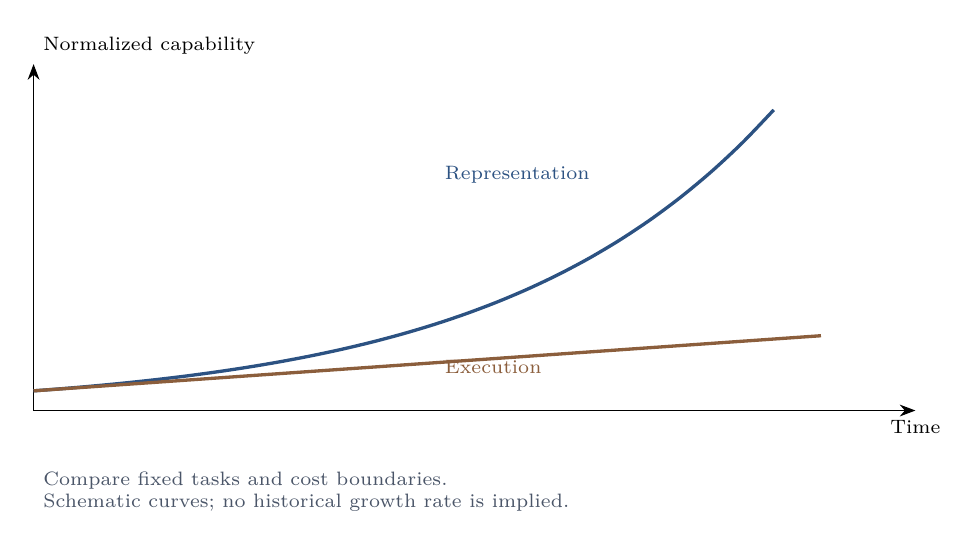
\begin{tikzpicture}[x=1cm,y=1cm,font=\scriptsize]
\draw[-{Stealth[length=2mm]}] (0,0)--(11.2,0) node[below]{Time};
\draw[-{Stealth[length=2mm]}] (0,0)--(0,4.4) node[above right]{Normalized capability};
\draw[deepblue,line width=1.2pt,domain=0:9.4,smooth] plot (\x,{0.25*exp(0.29*\x)});
\draw[terra,line width=1.2pt,domain=0:10,smooth] plot (\x,{0.25+0.07*\x});
\node[anchor=west,deepblue] at (5.1,3.0){Representation};
\node[anchor=west,terra] at (5.1,0.55){Execution};
\node[align=left,anchor=north west,text=slate] at (0,-0.65){Compare fixed tasks and cost boundaries.\\Schematic curves; no historical growth rate is implied.};
\end{tikzpicture}
\caption{Two speeds. A gain in producing representations can outrun the receiving system's capacity to execute them.}
\label{fig:two-speeds}
\end{figure}


\subhead{The installed world}

Moving from representation to matter introduces execution costs. A rendered vehicle follows a calculated trajectory. A real one needs energy, traction, braking, steering, sensing, and contact control. A bridge design can be revised quickly; building it requires materials, equipment, labor, and a suitable foundation. Steel strength, ground conditions, and concrete curing enter the same engineering account. The familiar 28-day concrete strength is a testing benchmark; mix, temperature, and curing methods affect the rate of strength development. Faster drawing changes one part of this chain.

The second constraint is the installed base. Software can sometimes be reorganized within a recoverable environment. Cities must be changed while people continue to live in them. Roads sit above buried services; new electrical loads connect to existing substations; a hospital's new equipment enters established clinical and maintenance routines. Upgrading a system requires a transition plan for the things that are already connected. Even a technology that needs little roadside modification must accommodate roads, users, operating rules, and liability.

A third constraint comes from operating conditions. A simulator contains the disturbances its designers have included. A deployed system encounters additional changes, failures, and participants. A road crew deals with subsidence, conflicting utility maps, access requirements, weather, and the needs of nearby residents. A driving system faces the conditions under which its sensing and control actually work. Simulation can expose many failures before deployment. Field performance still depends on the relation between the model and the operating environment.

\subhead{The cost of reversal}

Recoverability changes the price of experimentation. Restoring a simulation state can be routine. A demolished pier, an administered medicine, or a damaged battery requires a different remedy. Physical repair can be possible, but its resource cost and consequences do not disappear when a previous design file is restored. Methods developed for cheap retries must be evaluated against the failure costs of the receiving system.

Prediction and control also have different requirements. A system may predict that a falling glass will shatter. Catching it requires a sensor estimate, an actuator capable of reaching it, a suitable grip, and feedback fast enough to maintain contact without breaking it. Learned models can contribute to each part. Performance at representing an event does not establish performance at intervening in it.

As generated scenes become more convincing, the crew outside the window can seem increasingly clumsy. That comparison omits most of the crew's task. One system produces a plausible account of forces; the other must apply them under real constraints.

\key{A speed achieved in representation must be accounted for again at execution.} Energy, material properties, logistics, dependencies, and cooperation determine what crosses the boundary. These constraints can spread the effects of an abrupt improvement over a longer transition. They provide a buffer only when plans actually allow for them.

The difference between the screen and the street is visible. Why, then, does public judgment so often take the faster side as representative? Part of the answer lies in how technological examples are selected, displayed, and financed.

\subsection{The Technologies That Make the Demo}

\subhead{Selection by attention}

Software makes an unusually good demonstration. Its output can be shown, copied, and compared immediately. The construction of the building that houses the servers is harder to display as a breakthrough. Attention selects the lightest visible layer and leaves much of its support outside the frame.

The selection process reinforces itself. A result that can be demonstrated attracts attention and investment; those resources help produce the next demonstration. Meanwhile, fabrication, power delivery, cooling, and maintenance progress through other schedules. Each can improve substantially, but its rate has to be measured on its own terms.

An audience repeatedly shown the fast cases can mistake the sample for the whole. Then medicine, education, energy, and manufacturing are all expected to follow the trajectory of a software product. Slow adoption becomes evidence that an industry lacks digitization or that a model lacks intelligence. The possibility that another part of the system is binding drops out of view.

The omitted cases cannot correct the story quickly. A planning decision, a replacement transformer, a materials qualification, or an extended field test supplies feedback over months or years. Its silence during a product launch is easily read as absence.

\subhead{Infrastructure behind the interface}

Communications provide a familiar example. A signal indicator on a phone gives no sense of the work behind coverage. Fiber installation can require access agreements, trenching or duct access, coordination with other utilities, testing, and repair. A protocol update and a physical network upgrade have different critical paths. The distinction comes from the operations required, not from a universal ratio between the speed of electrons and the speed of atoms.

Energy systems make the issue sharper. A better dispatch algorithm can improve the use of available capacity. New capacity may still require equipment, land, financing, construction, network studies, and connection work. A hypothetical doubling of a solar panel's conversion efficiency would change the area or output calculation; it would still leave panels to manufacture, transport, mount, connect, and maintain.

Berkeley Lab's 2026 queue study gives the US example a scale: more than 2,060~GW of generation and storage capacity was seeking grid connection at the end of 2025. For the regions with data, projects completed in 2025 had a median interval of more than five years from request to commercial operation. Much of the queued capacity will never be built. A submitted project and an operating power supply are different states.\cite{berkeley2026queues}

Precision manufacturing poses the same distinction at a different scale. A lithography system can embody extraordinary informational sophistication while still requiring demanding fabrication, assembly, transport, installation, calibration, and service. Yield improvement depends on contact with materials and process variation. Better algorithms can shorten a feedback cycle and extract more from it. Evidence from the cycle remains part of the achievement.

\subhead{Where the cloud stands}

The word \emph{cloud} conceals an engineering site. Compute runs in buildings connected to electrical and communications networks, with servers, storage, power conversion, cooling, and staff. The IEA's October~14, 2026 report describes network capacity, connection queues, and permitting as constraints on data-center expansion.\cite{iea2026powering} The race for intelligence has reached the substation.

Cooling requirements depend on the architecture, location, and operating conditions. A facility may consume water directly; water use may also arise in the electricity supply chain. No single evaporation rate describes every data center. The general requirement is to carry away waste heat while keeping equipment within its operating limits.

The hardware has its own material history: mined inputs, processing, wafers, components, assembly, shipping, and replacement. Their costs can be made less visible to a user without being removed from the system.

This bias needs no coordinated deception. What can be demonstrated receives attention; what enables it is treated as background. A useful analysis must give both a place in the same account.

\subhead{Technological viscosity}

\term{Technological viscosity} is the generalized resistance encountered when intelligence, an algorithm, or a technical plan attempts to move a real system from state~A to state~B. Execution, verification, maintenance, coordination, and the handling of failure all enter it. The word borrows from fluid mechanics the idea of resistance arising within the medium. In this book, its broader use requires task-specific definitions and measurements.

Cheap generation changes the distribution of scarcity. When candidates multiply faster than reliable outcomes, trust and absorption capacity become relatively more valuable. A field once limited by its supply of possible designs may become limited by its ability to test, build, or sustain them. Candidate abundance can coexist with a shortage of results on which anyone can depend.

Three coordinates give the smallest useful starting framework: \term{resource barriers} ($R$), \term{temporal rigidity} ($T$), and \term{topological coupling} ($G$). Can the change be supplied with resources? Can the required processes unfold in time? Can the change propagate through the dependencies already in place? These questions recur throughout the book.

\subsection{The Material Basis of Virtual Escape}

\subhead{Moving inward}

When the material world is expensive and difficult to change, moving activity into a virtual environment can be attractive. High housing costs, congestion, and limited mobility give that attraction practical force. Remote work, online communities, and virtual environments can reduce particular travel or space requirements. The proposal becomes more ambitious when it treats mediation as independence from the physical conditions that sustain it.

An old aspiration returns in a new form: keep an elaborate inner world while reducing the body's demands to a minimum. A headset offers a beach without a flight; an online meeting offers contact without a commute. Some substitutions produce real savings. Their effect must be compared with the activities displaced and the infrastructure added.

The political version appears in proposals such as Balaji Srinivasan's \emph{The Network State}: organize online, then acquire a territorial and institutional presence. The relevant physical question is what supplies the energy, communications, transport, public health, and security on which the arrangement depends. A digital community can reorganize how these services are obtained. Independence requires an account of who actually provides them.

The same question applies to ordinary remote work. A person can leave an office while remaining dependent on a grid, a network, a supply chain, and emergency care. The visible location changes faster than the supporting system.

\subhead{The thermodynamic account}

A virtual environment is implemented by physical states: charges and voltages, magnetic or electronic storage, and optical signals. Contemporary computation and communication dissipate energy. Supplying power and removing waste heat are operating conditions of the service.

The sources and environmental effects of that electricity vary by place and time. Additional digital activity can increase demand; substitutions and efficiency improvements can reduce other demands. The net result requires a defined comparison. Virtual activity has a substrate even when it delivers a net material saving.

Spatial flexibility also requires spatial infrastructure. A remote worker's connection may run through local distribution equipment, terrestrial fiber, undersea cables, and distant data centers. Those assets require construction, protection, inspection, repair, and replacement. Redundancy and geographic recovery can make them more reliable at additional cost. Thermodynamics alone supplies no rule that a more ordered or more complex system must be more fragile.

The entropy balance for a system and its environment is

\begin{equation}
\Delta S_{\mathrm{system}}+\Delta S_{\mathrm{environment}}
=\Delta S_{\mathrm{total}}\geq 0.
\end{equation}

Each term has units of joules per kelvin. If their combined boundary is isolated, a local entropy decrease must be accompanied by an equal or larger increase elsewhere. Equality is the reversible limit. Real power conversion, cooling, manufacturing, and transport include irreversible processes.

Visual tidiness and informational usefulness are different quantities from thermodynamic entropy. A clean desktop is not a measurement of $\Delta S_{\mathrm{system}}$. The balance establishes the physical terms of the computation and its support, rather than a fixed entropy price per image, insight, or neatly arranged screen. Pollution, water consumption, and electronic waste also require their own measurements; they cannot be read directly from this inequality.

Much of the apparent lightness of digital life comes from a division of work and location. An interface presents the result while the supporting machinery, maintenance, heat rejection, and waste handling occur elsewhere. Some costs fall, some move, and some new ones appear. The account has to follow all three.

\subhead{The body remains connected}

Human participation adds a biological condition. There is no demonstrated method for uploading a person's consciousness and dispensing with the living body. Ordinary digital life therefore still depends on food, temperature regulation, sleep, care, and health. A wound heals through a biological process; replacing a file does not replace that process.

An apparently frictionless service can relocate bodily work. The electrical technician who maintains the supply, the parcel driver who reaches an inaccessible entrance, and the nurse who responds when someone becomes ill handle parts of the experience hidden by the interface. Their work has not become virtual because the request arrived through an app.

Digital mediation can change how much material support an activity needs. It cannot dispense with support altogether. A serious account of virtual freedom therefore follows its dependencies into power, equipment, maintenance, and living bodies.

So far, those dependencies have appeared as obstacles. They also perform another function. The same resistance that limits a rate of change can keep a system from coming apart. To see that function, we need to examine viscosity as damping.

\section{Resistance as a Stabilizer}

\subsection{The Physical Anchor}

Computation can advance abruptly while the systems it is meant to transform remain largely recognizable. A factory, a city, and a health service all absorb change through structures that already have work to do. The gap between a new capability and a transformed world is produced inside those structures.

Two processes matter: execution and confirmation. Execution meets resources, process time, and dependencies. Confirmation meets evidence, standards, and responsibility. Together they shape the transition from a technical possibility to something on which people act.

A damped oscillator gives the simplest picture of how a system's response depends on more than the force applied:

\begin{equation}
m\frac{d^2x}{dt^2}+\gamma\frac{dx}{dt}+kx=F(t),
\qquad
\zeta=\frac{\gamma}{2\sqrt{mk}},
\qquad
\tau_{\mathrm{slow}}\approx\frac{\gamma}{k}\quad(\zeta\gg1).
\end{equation}

For a mechanical displacement $x$, $m$ is mass, $\gamma$ the damping coefficient, $k$ the restoring stiffness, and $F(t)$ the driving force. Their units are kg, kg/s, kg/s$^2$, and N respectively. The damping ratio $\zeta$ is dimensionless. In the strongly overdamped regime, the slow relaxation time is approximately $\gamma/k$: more damping produces a longer transition.

As an analogy for technological change, inertia represents installed assets, damping represents resistance to transition, and restoring forces represent arrangements that maintain the existing state. For a constant input, the equilibrium displacement depends on $F/k$; the approach to it depends on the dynamic parameters. A force and a timetable are different parts of the model. Social and technical systems need their own measured variables before this analogy can yield a forecast.

Maintenance makes the distinction concrete. A body needs metabolism; a server needs power and cooling; a transport network needs inspection and repair. A building can persist for a time without an active supply, while its materials continue to age. These systems sustain order through different mechanisms and on different timescales. Work on an operating railway can be harder to schedule than work on an empty site because the railway must continue to carry people.

\subhead{Resource barriers}

Transforming matter requires a physical route. Ironmaking must reduce iron oxides. Cement manufacture must drive reactions and process material at high temperature. Furnaces, feedstocks, equipment, and heat flows belong in the account. Better chemistry and process design can lower actual energy use and sometimes alter the thermodynamic requirement by changing the route. An activation barrier, a reaction's free-energy difference, and a plant's energy consumption are distinct quantities. Computation earns its value by finding better routes through these conditions.

This is the resource barrier, $R$. A bridge requires materials and a site. A grid-control algorithm acts on a network whose generation, transmission, storage, and operating margins already exist. A robot policy runs through a battery, actuators, sensors, joints, and a maintenance system. Intelligence changes how resources are used. The resulting operation still needs resources.

Human bodies belong in the same comparison. Converting a daily food intake of 2,500 dietary kilocalories into average power gives

\begin{equation}
P_{\mathrm{human}}
=\frac{E_{\mathrm{food}}}{\Delta t}
=\frac{2500\times4.18\times10^3}{86400}
\approx1.2\times10^2\ \mathrm{W}.
\end{equation}

That is about 120~W of average metabolic input over a day. It supports the whole organism, including temperature regulation, cognition, and activity. Mechanical output is a different quantity.

A comparison with a machine requires the same task, duty cycle, quality, and system boundary. If a machine consumed an average of 1--3~kW under those conditions, its input-power ratio to 120~W would be about 8--25. Those machine values are an illustration. Equipment, labor, energy prices, downtime, and service life then determine the economic comparison.

A flexible human worker can be highly economical in an irregular setting. In a standardized operation, a specialized machine may reverse the comparison. The relevant protection comes from the present cost of completing the task.

\subhead{Temporal rigidity}

Every transition needs time to unfold. Heat must move, reactions must proceed, material damage must become observable, organisms must respond, and people must coordinate. This is temporal rigidity, $T$.

A candidate molecule and evidence about its long-term effects are separated by exposures and observations. A simulated traffic flow and a functioning transport service are separated by vehicles, maintenance, users, operating permissions, and practice. An infrastructure asset may be designed for decades of use, so a replacement must fit the service it is replacing.\cite{miatto2017how}

Parallel construction, prefabrication, better testing, and better coordination can shorten parts of a project. The useful analysis identifies which part of the critical path actually changes. Compress a year of design work to a day while leaving a multiyear build unchanged, and the number of proposed projects can grow much faster than the number completed.

Waiting also has more than one function. A redundant approval can be removed. An observation period may reveal a delayed effect. Consultation can expose a cost that a project sponsor would otherwise impose on someone else. Calling all three “delay” conceals the work each is doing.

\subhead{Topological coupling}

A system is a network of dependencies. A local improvement must pass through equipment, people, standards, routines, interests, and feedback. This is topological coupling, $G$.

A medical model enters a hospital's diagnostic workflow, record systems, staffing, reimbursement arrangements, and responsibility for treatment. A new energy device enters a grid. A better driving policy enters a road system used by other people. A strong component can fail to transform the whole because the surrounding connections do not support the transition.

Moravec's paradox draws attention to the difficulty of ordinary embodied performance. A formally specified game can demand immense search while still supplying explicit rules and a clear account of success. A robot handling laundry must cope with uncertain shape, occlusion, contact, friction, and deformation. The environment with the more complicated rules on paper can be easier to formalize.

Discretizing $n$ degrees of freedom into $m$ values each produces

\begin{equation}
N_{\mathrm{config}}=m^n,
\qquad
\ln N_{\mathrm{config}}=n\ln m.
\end{equation}

This count explains why exhaustive search rapidly becomes impractical. Geometry, learning, feedback, and passive mechanics can avoid that enumeration. The remaining difficulty depends on the task and the method. A person folding a shirt benefits from a body and a lifetime of interaction already fitted to the problem.

Standardizing the environment changes the comparison. A warehouse with regular containers, predictable shelving, and controlled access can be much easier to automate than an arbitrary home. Part of the achievement has been purchased by rebuilding the task's surroundings. Resource barriers and topological coupling move together.

\subhead{Three media}

Bits, atoms, and life absorb intelligence differently.

In the domain of \term{bits}, generated output can often become visible immediately. Text, images, code, data, and virtual scenes are easy to duplicate and revise within a recoverable environment. Trust imposes another threshold: reliable code, traceable knowledge, and decisions with an accountable owner require more than the arrival of an output.

In the domain of \term{atoms}, a prediction must become a force, a contact, a movement, or a flow. Manufacturing, construction, transport, energy, logistics, and robotics pay for mass, friction, inertia, strength, space, and maintenance. A wrongly cast component needs physical rework. An improved controller changes what machinery can do within those conditions.

In the domain of \term{life}, intervention changes a system that continues to respond. Cells, bodies, organisms, and ecosystems compensate, adapt, and sometimes evolve. AI can accelerate target identification, structural prediction, molecular design, and screening. Toxicology, pharmacokinetics, clinical effects, and sustained safety require evidence from the relevant biological processes. A gene's function depends on its regulatory, developmental, cellular, and ecological setting.

The basic pattern is uneven absorption. Bits support rapid diffusion, atoms require work, and life returns feedback. A model capability can move quickly through one layer and slowly through another.

\begin{figure}[ht]
\centering
\begin{tabularx}{\textwidth}{@{}lYYY@{}}
\toprule
 & \textbf{Bits} & \textbf{Atoms} & \textbf{Life}\\
\midrule
Absorption & Copy and diffuse & Apply force and move material & Respond and adapt\\
Main demands & Compute, evidence, trust & Energy, materials, maintenance & Regulation, exposure, sustained feedback\\
Reversal & Often cheap within a saved state & Repair and reconstruction & Recovery may be limited or delayed\\
Example & A patch in a test branch & A robot handling an object & A drug acting in a body\\
\bottomrule
\end{tabularx}
\caption{Three media, three ways of absorbing an intervention. The same project can span all three columns.}
\label{fig:media-gradient}
\end{figure}


Code acquires a much higher cost of failure when it controls a production system. A drug candidate enters a different timetable when it reaches a trial. The task and the consequence matter alongside the medium.

The three coordinates can trade against one another. More resources may buy time; more time may allow a lower-resource process; redundancy may improve reliability while adding equipment and maintenance. New processes can also reduce several costs together. A lighter user experience can conceal a heavier backend, while a genuine process improvement can reduce the total.

\key{Which resistance fell, and where did the rest go?} That question follows a technology beyond its demonstration.

\subsection{The Grounds for Relying on a Result}

Execution asks how a proposal reaches the world. Confirmation asks what warrants relying on it. A well-formed statement, a supported claim, and a successful intervention require different evidence.

\subhead{The verification pyramid}

A thousand drug candidates do not create a thousand trial programs. A large library of driving policies does not establish how any one behaves on public roads. A polished policy proposal does not establish its effects on organizations or public trust. Verification consumes resources, time, and access to the system being investigated.

Six layers make the progression visible. \term{Formal checks} test syntax, rules, and specified logical properties. \term{Semantic checks} examine meaning, facts, citations, and sources. \term{Causal tests} examine whether an intervention produces an effect. \term{Engineering validation} examines operation under noise, failure, maintenance, cost, and scale. \term{Long-term biological and human evaluation} examines effects that need time to emerge. \term{Accountability} asks whether a deployed arrangement can be explained, audited, challenged, and made to answer for harm.

For candidates filtered through successive stages,

\begin{equation}
N_k=N_0\prod_{i=1}^{k}p_i,
\qquad 0\leq p_i\leq1,
\end{equation}

where $p_i$ is the fraction passing stage~$i$ among those that passed all earlier stages. The expression follows from conditional counting, without an independence assumption. If a stage leaves no survivors, later counts remain zero. It counts survivors; the cost and reliability of each test require separate measures.

\begin{figure}[ht]
\centering
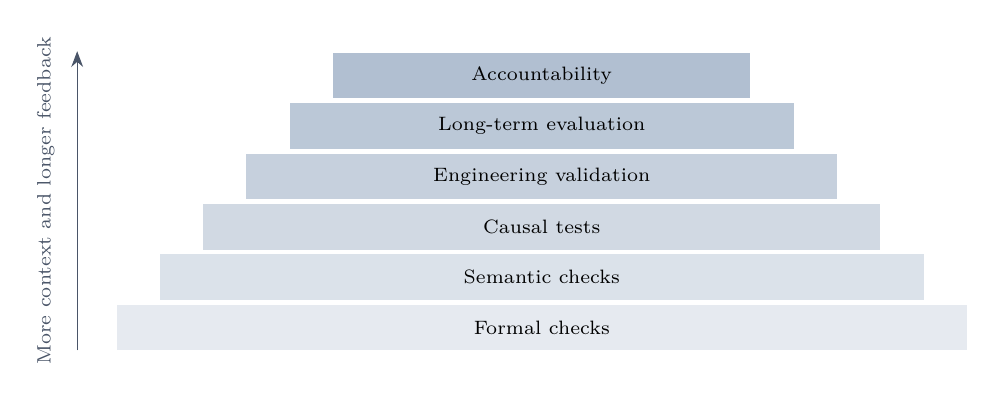
\begin{tikzpicture}[x=1cm,y=1cm,font=\scriptsize]
\foreach \y/\w/\shade/\tag in {0/10.8/12/Formal checks,0.64/9.7/17/Semantic checks,1.28/8.6/22/Causal tests,1.92/7.5/27/Engineering validation,2.56/6.4/32/Long-term evaluation,3.2/5.3/37/Accountability}{
  \fill[deepblue!\shade] (-\w/2,\y) rectangle (\w/2,\y+0.58);
  \node at (0,\y+0.29){\tag};
}
\draw[-{Stealth[length=2mm]},slate] (-5.9,0)--(-5.9,3.8);
\node[rotate=90,slate] at (-6.3,1.9){More context and longer feedback};
\end{tikzpicture}
\caption{Different questions require different evidence. The shape organizes the verification tasks; its widths are illustrative.}
\label{fig:verification-pyramid}
\end{figure}


Tools can improve every layer, at different rates. Automatic checks may increase throughput sharply. Field exposure, long-term observation, and the resolution of disputed consequences remain tied to other processes. When candidate generation outruns them, the waiting room fills.

The upper layers also change the standard of judgment. The acceptance conditions for a formal specification can be explicit. An accountable deployment must respond to the actual distribution of risks and interests. Operational rules can encode part of that task. Treating the encoded portion as the entire objective creates a new failure mode: participants learn to optimize the measure while the purpose recedes.

\subhead{Proof and its premises}

Gödel's incompleteness theorems establish limits for consistent, effectively axiomatized formal systems strong enough to express basic arithmetic. Under the relevant hypotheses, some propositions cannot be decided within the system; the second theorem restricts its ability to prove its own consistency.\cite{godel1931}

An engineering example brings the practical question closer. A proof that a program satisfies a specification leaves open whether the specification captures the intended requirement. Machines can check proofs and help check specifications. Sensors, tests, and independent evidence can extend the chain. The remaining judgment concerns what errors the chain covers and what its omissions would cost.

For decisions that allocate risk and benefits, standards also need authorization. People who bear the consequences need ways to provide evidence, contest a requirement, grant permission, and appeal a decision. Formal competence and legitimate authority answer different questions.

\subhead{A promise needs an address}

Trust includes a question that an accuracy score leaves unanswered: where does the loss go when the decision fails?

Nassim Taleb's idea of \emph{skin in the game} draws attention to the relation between decision makers and those exposed to their decisions. A person can pledge property, professional standing, and reputation. An organization can supply assets, a durable identity, insurance, and a structure for correction and compensation. These arrangements give a promise an address.

Medical and other consequential services need both reliable decisions and a workable response to failure. Records, review, suspension authority, and a responsible operator help establish that response. A human assigned to approve outputs needs the information, time, and power to intervene. A name on a form supplies little by itself.

Trust can also accumulate through a relationship. Care, counseling, and companionship involve memory, knowledge of a situation, and commitments that are kept over time. A model can generate a response. The service still has to establish continuity, crisis handling, and correction.

Evidence gives a judgment grounds; accountability gives a commitment a return path. Both can be supported by automation and institutions. Together with the conditions for execution, they stretch the transition from a new capability to a changed society.

The transition is a contested interval. Work can be reorganized on one timetable while people's account of their own worth changes on another. That mismatch is the next problem.

\section{The Crisis of Instrumental Value}

\subsection{Replacement Runs on Different Clocks}

Tasks are exposed to automation at different points in the chain. Generating routine text, summaries, code, and analysis often takes place in a low-friction environment. Repair, assembly, inspection, care, and transport require action within a setting that can be irregular, occupied, and consequential. A new model capability meets different deployment costs in each.

This creates a social split: \key{the body can remain in the old workplace while the evidence of professional worth has already changed.}

\subhead{The economics of the last meter}

A robot is a capital asset. Purchase, integration, depreciation, maintenance, power, supervision, and downtime enter its cost. Human labor has wages, benefits, training, safety, support, and the wider costs of developing and sustaining a person. An employer's account captures only part of the latter. A low purchase price for labor can reflect a successful transfer of costs to workers, households, or public institutions.

An introductory annual-cost comparison is

\begin{equation}
C_{\mathrm{human}}=w,
\qquad
C_{\mathrm{machine}}=\frac{K}{L}+m.
\end{equation}

Here $w$ is the annual cost assigned to the human option, $K$ the machine's purchase and installation cost, $L$ its accounting life in years, and $m$ annual operating and maintenance expense. For matched output, quality, availability, and risk, a lower $K/L+m$ can favor substitution in this simplified account. Financing, utilization, transition costs, and the distribution of liability can change the result. An attractive purchase calculation still needs an executable deployment.

The last meter often carries the irregular work. Consider a parcel route. Route planning is one task; finding the correct entrance, handling a damaged package, dealing with an inaccessible building, and resolving a disputed delivery are others. A warehouse robot meets a related problem when a container deforms or an object lies outside the expected pose. Each additional condition has to be engineered into a system that remains economical and reliable.

The field is advancing, so a frozen picture of robot failure would be misleading. On October~27, 2026, Waymo announced an expansion of nearly 250 square miles across five United States markets. A week earlier it announced preparations for Madrid; its Toronto announcement set a goal of first riders in 2028.\cite{waymo2026expansion,waymo2026madrid,waymo2026toronto} Existing service, a local expansion, and a future launch target occupy different stages of the same deployment chain. Reading them all as a single capability number erases most of the engineering.

\begin{figure}[ht]
\centering
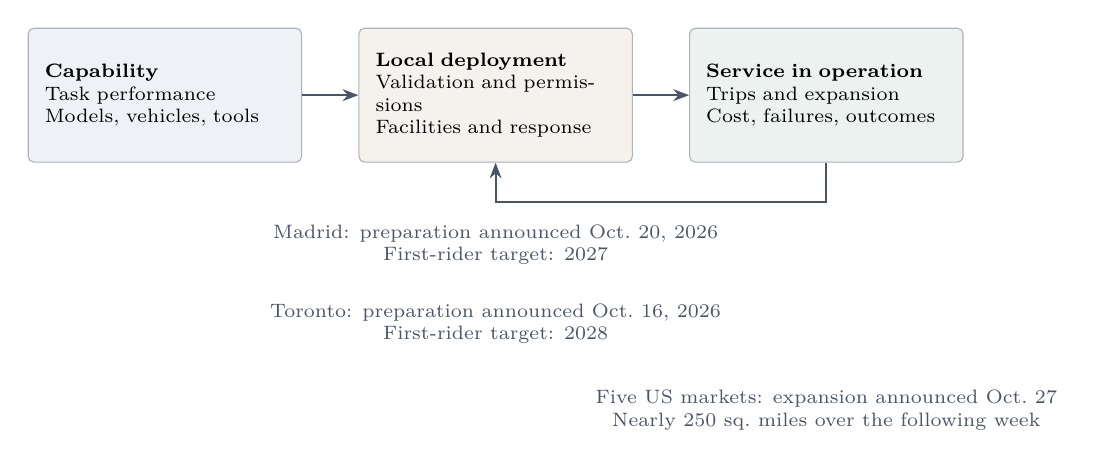
\begin{tikzpicture}[x=1cm,y=1cm,font=\scriptsize,
box/.style={draw=slate!45,rounded corners=2pt,align=left,inner sep=6pt,text width=3.05cm,minimum height=1.7cm},
arr/.style={-{Stealth[length=2mm]},line width=0.8pt,slate}]
\node[box,fill=deepblue!8] (a) at (0,0) {\textbf{Capability}\\Task performance\\Models, vehicles, tools};
\node[box,fill=terra!9] (b) at (4.2,0) {\textbf{Local deployment}\\Validation and permissions\\Facilities and response};
\node[box,fill=forest!9] (c) at (8.4,0) {\textbf{Service in operation}\\Trips and expansion\\Cost, failures, outcomes};
\draw[arr] (a)--(b);
\draw[arr] (b)--(c);
\draw[arr] (c.south) -- ++(0,-0.5) -| (b.south);
\node[align=center,text=slate] at (4.2,-1.9) {Madrid: preparation announced Oct.\ 20, 2026\\First-rider target: 2027};
\node[align=center,text=slate] at (4.2,-2.9) {Toronto: preparation announced Oct.\ 16, 2026\\First-rider target: 2028};
\node[align=center,text=slate] at (8.4,-4.0) {Five US markets: expansion announced Oct.\ 27\\Nearly 250 sq.\ miles over the following week};
\end{tikzpicture}
\caption{Capability, deployment, and operation are different kinds of progress. Examples follow Waymo's October 2026 announcements; targets retain their status as plans.}
\label{fig:deployment-stages}
\end{figure}


Substitution also has a calendar. Procurement, installation, qualification, retraining, and a new operating arrangement consume time after a machine demonstrates a task. The ratio between that interval and the time needed to generate a plan depends on the task. Cheap generation does not install a fleet.

These cost advantages move. Better machines, higher utilization, lower energy prices, and standardized environments can reverse a comparison. The buffer is an opportunity to organize a transition.

\subhead{Useful, but no longer the author}

Employment can persist while its meaning changes. A person's job may survive because the receiving system is hard to automate, even as the outputs used to recognize their expertise become easy to obtain elsewhere.

Employment statistics and professional experience then register different things. One counts whether a position exists. The other asks whether the position still conveys competence, discretion, and recognition. A worker can remain on the payroll while losing authority over the process.

Modern institutions often reward people through a functional equation: ability, output, and social standing are treated as if they rose together. Generative systems disturb the relation. A finished illustration or a plausible program no longer provides the same evidence of training and experience. Expert judgment can remain valuable while the familiar artifact becomes a weaker signal of it.

The resulting fear can exceed a fear of lost income. “Someone can still pay me to do something” does not settle “what part of this work is mine?” Where outputs once established a place, their abundance creates a demand for other forms of proof.

Algorithmic management makes this problem visible. In parcel logistics, warehouse picking, and ride-hailing, software can assign tasks, shape routes, record performance, and influence pay, while people handle the physical contact and its exceptions. The degree of autonomy depends on the power to refuse, revise, contest, or pause a task. A worker can be indispensable to execution and have little say over its terms.

Yuval Harari's phrase “useless class” points toward the anxiety, but usefulness can remain high. People may still perform necessary work while disappearing from the account of who directs and creates. The question is their recognized agency within the system.

The danger is a split between bodily usefulness and public authorship. A society may continue to depend on people for difficult material work while describing intelligence and initiative as properties of the coordinating platform. Addressing that split requires more than keeping jobs numerically intact.

\subsection{Efficiency Creates New Bottlenecks}

An efficiency gain creates room for a response. That response can consume the room.

Cheap generation supplies more proposals, drafts, and code. If their arrival rate grows faster than review and maintenance capacity, work accumulates there. The person spared a first draft may inherit a queue of drafts to judge. This is a throughput mismatch; a saving can also remain a saving when the receiving system has enough capacity.

\begin{figure}[ht]
\centering
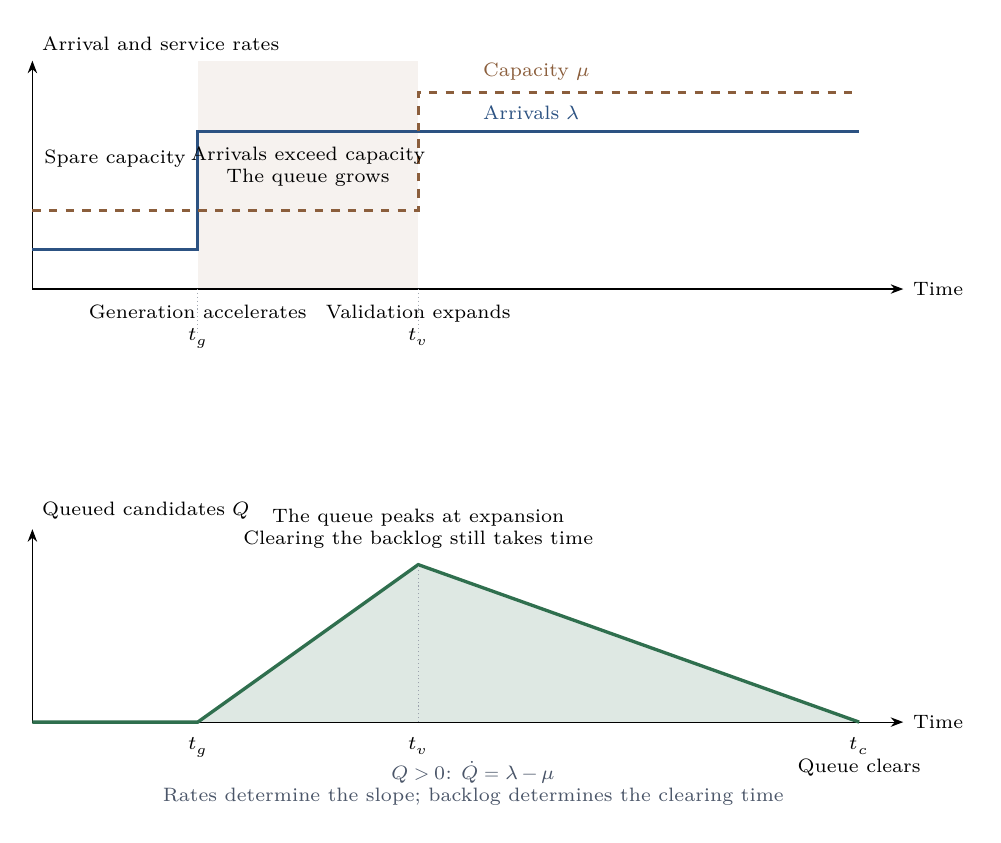
\begin{tikzpicture}[x=0.7cm,y=0.50cm,font=\scriptsize]
\fill[terra!8] (3,0) rectangle (7,5.8);
\draw[-{Stealth[length=1.6mm]}] (0,0)--(15.8,0) node[right]{Time};
\draw[-{Stealth[length=1.6mm]}] (0,0)--(0,5.8) node[above right]{Arrival and service rates};
\draw[deepblue,line width=1.2pt] (0,1)--(3,1)--(3,4)--(15,4);
\draw[terra,dashed,line width=1.2pt] (0,2)--(7,2)--(7,5)--(15,5);
\node[deepblue,anchor=south west] at (8,4.05){Arrivals $\lambda$};
\node[terra,anchor=south west] at (8,5.05){Capacity $\mu$};
\node[align=center] at (1.5,3.3){Spare capacity};
\node[align=center] at (5,3.1){Arrivals exceed capacity\\The queue grows};
\draw[slate!50,densely dotted] (3,0)--(3,-1.1);
\draw[slate!50,densely dotted] (7,0)--(7,-1.1);
\node[anchor=north,align=center] at (3,-0.15){Generation accelerates\\$t_g$};
\node[anchor=north,align=center] at (7,-0.15){Validation expands\\$t_v$};
\begin{scope}[yshift=-5.5cm]
\fill[forest!16] (3,0)--(7,4)--(15,0)--cycle;
\draw[-{Stealth[length=1.6mm]}] (0,0)--(15.8,0) node[right]{Time};
\draw[-{Stealth[length=1.6mm]}] (0,0)--(0,4.9) node[above right]{Queued candidates $Q$};
\draw[forest,line width=1.2pt] (0,0)--(3,0)--(7,4)--(15,0);
\draw[slate!55,densely dotted] (7,0)--(7,4);
\node[anchor=south,align=center] at (7,4.15){The queue peaks at expansion\\Clearing the backlog still takes time};
\node[anchor=north] at (3,-0.15){$t_g$};
\node[anchor=north] at (7,-0.15){$t_v$};
\node[anchor=north,align=center] at (15,-0.15){$t_c$\\Queue clears};
\node[align=center,text=slate] at (8,-1.55){$Q>0$: $\dot Q=\lambda-\mu$\\Rates determine the slope; backlog determines the clearing time};
\end{scope}
\end{tikzpicture}
\caption{A moving bottleneck. Arrival rate $\lambda$ exceeds service capacity $\mu$ after generation accelerates. Later capacity expansion reverses the slope, but clearing the queue takes time. Schematic, with uncalibrated vertical scales.}
\label{fig:bottleneck-migration}
\end{figure}


Several familiar mechanisms expose the same pattern. Table~\ref{tab:ch1-paradox} places them side by side.

\begin{table}[ht]
\centering
\caption{Local improvements and the responses they can induce}
\label{tab:ch1-paradox}
{\small
\begin{tabularx}{\textwidth}{@{}p{2.25cm}YYY@{}}
\toprule
Mechanism & Local change & Response & Possible result\\
\midrule
Jevons & Cheaper use & More uses and users & Higher total consumption\\
Braess & An added route & Drivers reroute & A worse traffic equilibrium\\
Goodhart / Campbell & A rewarded metric & Behavior targets the measure & The measure loses fidelity\\
Lucas / reflexivity & A model informs action & Participants adapt & Historical relations change\\
Risk compensation & Lower risk per exposure & More or stronger exposure & Some benefits are offset\\
Automation irony & Routine tasks disappear & People move away from practice & Harder exceptional takeovers\\
\bottomrule
\end{tabularx}}
\end{table}

The common sequence is a changed local condition, a response within the system, and a new distribution of costs. The mechanisms remain distinct. Putting them in one account helps identify what a local performance measure misses.

\subhead{Use and equilibrium}

Jevons observed that more efficient use of coal could expand the activities that consumed it.\cite{jevons1865coal,allwood2012sustainable} Lower cost opens applications that were previously uneconomical. The outcome depends on how much use expands.

Let $q$ be the physical resource required per operation, $p$ the monetary price per operation, and $N(p)$ the number of operations per unit time. Under the illustrative assumption $p=\alpha q$ with fixed $\alpha$,

\begin{equation}
E=qN(p),
\qquad
\varepsilon=-\frac{d\ln N}{d\ln p},
\qquad
\frac{d\ln E}{d\ln q}=1-\varepsilon.
\end{equation}

$E$ is resource use per unit time and $\varepsilon$ the demand elasticity. For $\varepsilon<1$, lower resource use per operation reduces the total. For $\varepsilon>1$, expanded demand more than offsets the saving. The price relation connects engineering efficiency to demand in this example.

The current AI industry supplies a live version of the question. In April~2026, the IEA reported a steep fall in energy use per AI task alongside a 17\% increase in total data-center electricity demand during 2025. New use cases and adoption were expanding as individual tasks became more efficient.\cite{iea2026questions} Per-task efficiency and aggregate demand can move in opposite directions.

Generated code, content, and plans can exhibit a related throughput effect. Easier production invites more production. Review, testing, dependency management, and the disposal of bad candidates then become larger parts of the work. Whether the total burden rises is an outcome to measure.

Braess's paradox moves the issue from volume to routing. In some networks, adding an edge makes the equilibrium travel time worse because travelers adjust their routes in response.\cite{braess1968}

For one origin-destination pair and fixed demand, a Wardrop equilibrium requires every used route to have minimum cost:

\begin{equation}
f_i>0\ \Longrightarrow\
c_i(\mathbf f)=\min_{j\in\mathcal P}c_j(\mathbf f).
\end{equation}

By contrast, a system optimum minimizes total travel time over feasible flows:

\begin{equation}
\min_{\mathbf f\in\mathcal F}
\sum_{e\in E}f_e c_e(f_e).
\end{equation}

Here $f_e$ is edge flow, $c_e$ travel time on that edge, $\mathcal P$ the set of routes, and $\mathcal F$ the feasible flows satisfying demand and flow conservation. Route flow and edge flow are related by the network's incidence structure.

An added edge expands the feasible set, so it cannot worsen the system optimum when leaving the edge unused remains possible. It can worsen the equilibrium reached by independent route choice. More available options and a better collectively chosen outcome are separate properties.

Software tools can induce an analogous question: what happens when every participant adopts the locally attractive route? A tool's advantage for its first users may become a system's next queue.

\subhead{Measures and models}

Goodhart's and Campbell's observations concern measures that become targets.\cite{goodhart1975problems,campbell1979assessing} Once a score governs rewards, staffing, access, or reputation, participants have a reason to reshape their behavior around it.

A test-coverage percentage can rise without covering the dangerous failures. A support team can close tickets faster while transferring unresolved work to customers. A hospital metric can change which cases receive attention. The measured variable enters the control loop.

Verification systems face the same problem. Improving the resolution of a score helps while the score remains connected to the objective. A strong incentive to optimize the proxy can make that connection weaker.

The Lucas critique asks what happens when a policy changes the behavioral relations used to predict its effects.\cite{lucas1976econometric} Reflexivity emphasizes how participants' beliefs and actions can help shape the object they describe.\cite{soros1987alchemy} A risk model can influence the positions institutions take; a public forecast can change demand; a staffing model can alter the behavior it is later asked to explain.

Once a prediction becomes an input to action, it becomes part of the next state. A useful model must therefore be evaluated in use, including the responses its use induces.

\subhead{Risk and the work left over}

Risk compensation concerns changes in exposure after a safety improvement.\cite{peltzman1975effects} A lower chance of failure per event can encourage more events, higher speed, more leverage, or less attention.

With exposure rate $n$, failure probability $p$, and mean loss per failure $d$,

\begin{equation}
\mathcal R=pnd,
\qquad
d\mathcal R=nd\,dp+pd\,dn
\quad(d\ \mathrm{held\ constant}).
\end{equation}

For a small reduction in $p$ and increase in $n$, expected loss falls to first order when

\begin{equation}
\frac{|dp|}{p}>\frac{dn}{n}.
\end{equation}

The severity $d$ and the distribution of exposure also matter. A gain for one group can be accompanied by a cost to another. Risk compensation has to be assessed in its setting.

Automation changes the distribution of tasks. Bainbridge's \emph{Ironies of Automation} describes a persistent difficulty: routine operations disappear from human practice, while unusual failures demand a rapid and skilled takeover.\cite{bainbridge1983ironies}

People can perform fewer interventions and face a harder average intervention. They may have less recent experience of the process and less time to reconstruct its state. On-call engineering makes the structure familiar: an automated service can run quietly for a long time, then deliver an exceptional incident to someone who must diagnose it under pressure.

More capable AI can absorb a larger share of routine judgment. The remainder may then contain a higher concentration of ambiguous, consequential, and poorly documented cases. Deployment has to provide enough authority, information, practice, and time for the role it leaves to people.

\subhead{Where the pressure goes}

These mechanisms concern different variables: demand, route choice, incentives, expectations, exposure, and task distribution. Their shared lesson is a method of inquiry. After a local improvement, follow the system's response.

Where does the extra volume go? Which equilibrium becomes attractive? What does the metric now reward? What changes when the forecast is believed? Who takes the additional risk? Who handles the exceptional case?

Viscosity can move between locations: from energy to cooling, generation to verification, routine execution to incident handling, and local performance to coordination. Total cost can fall as well. An account that only records the improved component cannot distinguish those outcomes.

Energy supply and aging infrastructure add another constraint. Net usable energy depends on the technology, location, and boundary used to count energy invested in obtaining it. Maintenance depends on the condition of assets and the service required of them. Those costs need to be followed alongside demand.

The mature question is how the new operating arrangement performs after people and organizations have responded. The local improvement starts the analysis.

\subsection{After the Age of the Better Tool}

\subhead{Who bears the transition}

Costs move unevenly. A new process can remove friction from a customer's experience while adding pressure to a driver, an operator, a clinician, or a maintainer. Whether total efficiency improves and whether the distribution is acceptable are separate judgments.

Digital payments, navigation, simulation, automated experiments, and coding tools have delivered substantial gains. Political choices, capital markets, institutional competence, and culture shape what happens to those gains. The viscosity framework follows the material and organizational passage from an available capability to an outcome people can use.

\subhead{Three entangled paradoxes}

The first is the efficiency paradox of personal value. When a person's place rests entirely on outperforming a tool, a better tool makes that place precarious. Training and expertise can remain useful while becoming a less secure basis for recognition. A person cannot obtain a durable claim to dignity by winning every future benchmark.

The second is the escape paradox. Virtual freedom still needs equipment, energy, networks, maintenance, and bodies. Moving an activity online can reduce its material demands. It also rearranges the dependencies through which that freedom is supplied.

The third is the meaning paradox. A person may lose the pride of authorship while remaining necessary to keep the physical system running. The role offers usefulness without enough control, responsibility without enough authority, or income without recognition. The space between a useful component and a free participant becomes politically important.

\subhead{From performance to a place in the world}

These problems change the question. Alongside “How can I perform this task better?” comes “What can establish my place when the output is widely available?”

Judgment, responsibility, relationships, and the power to accept or refuse consequences supply parts of an answer. Their value depends on arrangements that make those powers real. A nominal human supervisor who cannot stop a system has little authority to exercise.

The material lag provides time to build such arrangements. The window moves as machines improve, costs change, and environments become easier to automate. It offers a transition interval, with no automatic settlement at its end.

History supplies repeated migrations of the evidence of value. Writing changed the role of memory. Printing changed access to texts and the institutions of interpretation. Steam power changed the place of muscular work. Computers changed the value of executing explicit rules. Generative systems are changing the evidential role of symbolic output.

Each transition created new roles and destroyed old ones unevenly. A displaced copyist did not automatically become an editor; an artisan did not automatically become an engineer. Access to the new role had to be built and contested.

The same will be true of verification, authorization, care, and responsibility. Platforms can absorb these roles, contracts can divide them, and institutions can concentrate them. Scarcity alone gives no guarantee that people who do the work will control it or receive its value.

The practical task is to connect technical capability with reliable execution and legitimate participation. Remove wasted work. Improve evidence. Give authority to the people expected to intervene. Establish where consequences return. A society's ability to generate alternatives becomes useful when it can choose, enact, and sustain them.

One question remains underneath the account. Why did intelligence arise in a world organized by energy gradients, dissipation, and material constraint? Until that is answered, the constraints can look like an obstacle placed in its way. The next chapter starts from their role in its origins.

\furtherreading{
Kurt Gödel, \textit{On Formally Undecidable Propositions of Principia Mathematica and Related Systems}\\
Hans Moravec, \textit{Mind Children}\\
W. Stanley Jevons, \textit{The Coal Question}\\
Dietrich Braess, “On a Paradox of Traffic Planning”\\
Donald T. Campbell, “Assessing the Impact of Planned Social Change”\\
Sam Peltzman, “The Effects of Automobile Safety Regulation”\\
Lisanne Bainbridge, “Ironies of Automation”\\
Nassim Nicholas Taleb, \textit{Skin in the Game}}

\chapter{The Physical Boundaries of Change}

Intelligence did not arrive in a weightless world and then discover that matter was inconvenient. It arose in a world where mistakes cost energy, time, injury, and lives. Its ability to rehearse an action before attempting it makes sense against that background. Resistance belongs in the explanation of intelligence's origins.

\section{Intelligence as a Path Selector}

\subsection{Gradients, Organisms, and Possible Routes}

\subhead{Order with a supply line}

A temperature difference, a chemical gradient, or a difference in pressure gives a process a direction. Open systems can use such gradients to maintain local structure while increasing entropy in their surroundings. A living organism inhabits this arrangement continuously. Stop its supply and waste removal, and its organization eventually fails.

Schrödinger's question in \emph{What Is Life?} was how an organism avoids rapidly settling into equilibrium. His memorable language of “negative entropy” pointed toward the material exchange that makes continued organization possible.\cite{schrodinger1944} In contemporary terms, the organism uses available free energy and exchanges matter and heat with its environment.

Prigogine and Nicolis studied how nonlinear, open systems driven away from equilibrium can develop organized patterns.\cite{prigogine1977nobel,nicolis1977} The pattern is sustained by its operation: a flow can maintain a structure that would not persist under equilibrium conditions. This supplies a physical setting for discussing life without making life a mechanical consequence of one thermodynamic formula.

Maximum-entropy-production proposals explore stronger claims about which organized states are selected. Their reach remains contested.\cite{martyushev2006,bruers2007} The argument here needs the more modest result: local organization and overall dissipation can grow together. Order can organize a route by which a gradient is discharged.

\subhead{A structure that helps make itself}

Autocatalysis adds persistence. Suppose a reaction produces a component that helps the network produce more of that component. With suitable supplies and conditions, a transient arrangement can reinforce itself. Kauffman's work on autocatalytic networks asks how mutually supporting reactions can become a system rather than a succession of isolated events.\cite{kauffman1993}

Such a network needs more to approach life: a boundary, a way of retaining and varying information, reproduction, selection, and regulation. Work on autocatalytic sets makes these distinctions explicit.\cite{hordijk2018} A reaction that accelerates itself is a promising ingredient, not an organism.

The RNA-world hypothesis offers one route toward connecting information and catalysis. RNA can carry sequence information and, in some arrangements, catalyze reactions. Gilbert's proposal gave a name to a hypothetical stage in which those roles were less sharply divided than they are in modern cells.\cite{gilbert1986} The history remains under investigation. The structural requirement is clear: a successful lineage has to connect supply, chemistry, boundaries, and inheritance tightly enough for improvements to accumulate.

\subhead{A landscape of possibilities}

An industrial process can be represented as a trajectory through a state space. Temperature, pressure, composition, geometry, inventory, equipment condition, and delivery schedule describe different coordinates. A feedstock occupies one region, a usable product another. Process design chooses a route between them.

Mechanics supplies a famous but distinct variational description:

\begin{equation}
S[q]=\int_{t_1}^{t_2}(T-V)\,dt,\qquad \delta S=0.
\end{equation}

$S$ is action in joule-seconds, $q$ denotes generalized coordinates, and $T$ and $V$ are kinetic and potential energy. Under the specified endpoint conditions, the physical path makes the action stationary. Stationarity does not always mean a minimum, and dissipation needs additional treatment.

Engineering optimization chooses an objective instead: cost, risk, energy, yield, or a combination. The two kinds of optimization must remain distinct. Physics does not guarantee that a factory, a nervous system, or an optimizer finds the cheapest possible route.

The useful image is a landscape. A route can waste fuel, overlook a catalyst, expose a worker to danger, or hold inventory that will never be used. Better information can change the route before anyone pays those costs. It changes the passage through the terrain.

\subsection{The Price of a Mistake}

\subhead{Rehearsal before collision}

Evolution conducts experiments in matter. A variation changes an organism; an unsuccessful action consumes energy, loses an opportunity, or causes injury. Selection can explore over many generations, but a particular animal cannot afford to test every cliff, predator, and unfamiliar food with its body.

A nervous system makes another kind of experiment possible. It can compare likely actions internally, discard some, and attempt a smaller set in the world. Learning adds the history of previous encounters. Intelligence, in this account, shifts part of the search from costly external action into comparatively cheap internal rehearsal.

\key{One of intelligence's oldest jobs is to avoid expensive mistakes.} This gives prediction and reasoning their practical place. Their value comes from improving action under a limited budget, including the cost of acquiring and processing information.

\subhead{Two meanings of entropy}

Shannon entropy measures uncertainty in a specified probability distribution.\cite{shannon1948} Thermodynamic entropy describes physical states and their transformations. Learning can reduce an agent's uncertainty without imposing a corresponding numerical decrease in the thermodynamic entropy of the outside world. A useful prediction has to be implemented in a physical system, but its usefulness is not measured in joules per kelvin.

The brain pays a substantial energy bill. Raichle and Gusnard's account places its consumption at roughly a fifth of the body's energy use, despite its much smaller share of body mass.\cite{raichle2002} Its advantage is an exchange: spend resources on perception, memory, and prediction to avoid more costly actions.

Landauer's result identifies a minimum heat cost for resetting a bit under the usual thermodynamic conditions, $k_{\mathrm B}T\ln2$.\cite{landauer1961} Actual computation operates above that idealized limit and pays for many other operations. The result connects information processing with its physical implementation; it does not provide a direct calorie count for a thought.

Friston's free-energy principle brings perception, action, and learning into a framework for maintaining viable states.\cite{friston2010} Its variational free energy is an information-theoretic quantity; a shared name does not make it identical to a fuel supply or a Gibbs-energy difference. The connection relevant here is the feedback loop: organisms predict and act as part of remaining alive.

\subhead{The route changes the barrier}

Material transformation presents two bills that should be kept separate. A reaction has kinetic barriers along a route and a thermodynamic relation between its initial and final states. Catalysts alter routes and reaction rates. They do not change the equilibrium free-energy difference for unchanged states.

Ironmaking requires reduction, heat transfer, materials handling, and equipment. A blast furnace pays these costs in a particular way; another reduction route changes the account.\cite{babich2021blast} Cement manufacture likewise combines reaction requirements with the losses of a real kiln. Process analyses distinguish the theoretical heat requirement from actual fuel use and auxiliary demand.\cite{madivate1999theoretical,madlool2011cement}

Calling every energy cost “activation energy” loses the distinction that makes engineering improvement intelligible. Catalysis can reduce a kinetic barrier. Heat recovery can reduce losses. A new feedstock can change the initial state. Each is a different way of improving the route.

\subhead{The continuing rent}

Maintenance is the other bill. Machines wear, structures corrode, organisms metabolize, and operating environments disturb the states a system needs to preserve. The book calls this continuing burden an \term{entropy tax}: an accounting image for the resources spent sustaining useful organization.

Different structures pay it on different schedules. A stone arch can remain standing without continuous active input. A refrigerated store cannot maintain its temperature that way. Distance from equilibrium alone does not determine the maintenance cost. Materials, disturbances, operating conditions, and the required function do.

Redundancy belongs in this account. An additional load path in a bridge may contribute only under an unusual event, yet its contribution can justify the material. A safety factor is not a universal instruction to double every component. It expresses uncertainty, design requirements, and the consequences of failure through a particular standard.

\subsection{From Representation to Transformation}

\subhead{A small signal, a large supply}

Language, maps, mathematics, and simulation extend rehearsal beyond one organism. A bridge calculation can reject dangerous designs without destroying bridges. An experiment can eliminate a drug candidate before broader exposure. An organization can learn from another organization's failure.

AI increases the density of this preliminary search. It can explore many candidate routes, infer relations, and propose alternatives. The useful result remains a selected route that a receiving system can execute.

A small control signal can govern a large power flow. One can describe successive power ratios as

\begin{equation}
P_k=P_0\prod_{i=1}^{k}G_i,\qquad G_i=\frac{P_i}{P_{i-1}}.
\end{equation}

The identity counts the ratios. Where a stage amplifies power, its energy comes from that stage's supply. A control signal tells an actuator what to do; a battery, fuel source, or grid supplies the work. Energy cannot be obtained by multiplying instructions.

The distinction also clarifies Maxwell's demon. Acquiring, using, and resetting information belong to the full physical cycle. The demon's discrimination cannot be removed from the account while the beneficial state change remains.

\subhead{Four inputs with different dimensions}

The ingredients of an engineered transformation can be written schematically:

\begin{equation}
\begin{gathered}
\text{Information: a recipe and control}\\
\text{Matter: a suitable carrier}\\
\text{Available energy: a supply for the process}\\
\text{Time: an interval in which it unfolds}
\end{gathered}
\quad\longrightarrow\quad
\begin{gathered}
\text{A functional structure}\\
\text{Waste heat and other outputs}.
\end{gathered}
\label{eq:conservation}
\end{equation}

This is a process account. Bits, kilograms, joules, and seconds cannot be added as one conserved quantity. Mass, energy, and entropy have their own balances, with the actual boundary and exchanges specified.

The practical point is stronger than a verbal “law of cost conservation.” A missing input can stop a correct plan. Information can reduce material waste or process time, but a recipe without an adequate carrier and an executable route remains a recipe.

\subhead{Candidate abundance}

Better search enlarges the set of proposals much faster than it necessarily expands testing and execution. A thousand building designs still compete for sites, crews, and capital. A thousand molecules compete for synthesis, assays, and evidence. A robot policy competes for hardware time and safe contact with its environment.

Computation has its own receiving system: chips, facilities, power, cooling, networks, and maintenance. Replacing an expensive physical experiment with a cheaper computational one can be an enormous gain. The gain is established by comparing complete routes.

Intelligence lets a system move some of the cost of choice ahead of the cost of action. Technological viscosity examines the rest of the journey: how a selected possibility becomes an actual, sustained change.

\section{Resource Barriers: Power, Matter, and Availability}

A resource is matter in a usable condition. A periodic-table entry is not a supply chain. Silicon in rock is not a wafer, atmospheric nitrogen is not fertilizer, and a metal dispersed through discarded products is not a stock of qualified components.

Extraction, concentration, purification, transport, fabrication, and maintenance create availability. A technical system builds its resource base as it uses it. This makes resources historically changeable without making their conditions optional.

\subsection{Power and the Rate of Change}

\subhead{Energy needs an appointment}

An energy total says little about whether a task can be done here, now, at the required rate. A process needs a form of energy it can use, delivered at a location, through equipment, within a time window. A reservoir of fuel, a charged battery, a live electrical connection, and heat at a low temperature provide different capabilities.

Kardashev's civilization types made controllable power a way of imagining technological scale.\cite{kardashev1964transmission} A commonly used continuous interpolation is

\begin{equation}
K=\frac{\log_{10}P-6}{10},
\label{eq:kardashev}
\end{equation}

with $P$ in watts. A rise of one unit corresponds to ten orders of magnitude in power; a rise of 0.1 corresponds to one. The logarithm keeps an enormous range on one axis. It says little about what is done with the power.

The chemical and nuclear energy scales differ greatly. Chemical reactions rearrange electrons; fission and fusion alter nuclei. Nuclear electricity, hydropower, wind, and solar already show why civilization's power cannot be described as a single chemical-bond ceiling.\cite{jaffe2018physics,smil2017energy} Converting a source into controlled, affordable output introduces equipment, supply, waste, and operating constraints.

Deuterium-tritium fusion releases about 17.6~MeV per reaction. Making useful power from it requires a favorable balance among heating, reaction output, confinement, material survival, and the rest of the plant.\cite{atzeni2004physics} High energy per event is a starting condition for an engineering program, not a deployed power station.

\subhead{A rocket's account}

Chemical propulsion supplies a sharp example of an energy route imposing a mass penalty:

\begin{equation}
\Delta v=v_e\ln\frac{m_0}{m_f},
\qquad
\frac{m_0}{m_f}=\exp\left(\frac{\Delta v}{v_e}\right).
\end{equation}

$v_e$ is effective exhaust velocity, and $m_0/m_f$ the initial-to-final mass ratio. In this idealized relation, every additional $v_e$ of required velocity change multiplies the mass ratio by $e$. Real missions also encounter gravity and drag losses. Staging and other propulsion systems change the design problem; the exponential explains the severity of the chemical route's tradeoff.

The same lesson applies less dramatically to machines on Earth. A controller can know a desirable motion while the actuator lacks peak power or the energy store lacks endurance. Intelligence and available power are different entries in the account.

\subhead{Storage, computation, and the wrong comparison}

Battery specific energy and a fuel's heating value measure different parts of a working system. Electric and combustion drivetrains convert stored energy with different efficiencies; tanks, packs, motors, cooling, and operating conditions also matter.\cite{placke2017lithium,ziegler2021reexamining} Quoting the ratio of two storage figures is useful only after establishing what is being compared.

Computing limits such as those studied by Bremermann and Bekenstein operate under particular physical assumptions.\cite{bremermann1982minimum,bekenstein1981universal} They are not forecasts of near-term chip improvement. A very distant theoretical limit neither guarantees cheap progress toward it nor tells a robot how much power its joints require.

Four groups of conditions recur: a suitable material, an available energy supply, a controllable process, and a way to sustain the result. Material selection and thermodynamics make their interaction visible.\cite{callen1985thermodynamics,georgescu1971entropy} A powerful source without suitable equipment can be unusable; an elegant process without stable feedstock can be uneconomic.

\subsection{Borrowing Structures That Nature Already Built}

\subhead{The first inventory}

Wood arrives with a fibrous structure. Cotton arrives with useful cellulose. A river arrives with a flow and a drop in height. An animal arrives with metabolism, muscles, and control. Early technologies often began by selecting and arranging such structures rather than synthesizing their properties from simpler feedstocks.

This is an advantage supplied by history. Photosynthesis, evolution, and geology have already performed some of the work. The user still pays for access, processing, transport, and renewal.

As requirements grow, those inherited forms become insufficient. A natural fiber may not have the required strength; a naturally occurring material may not have the purity a device needs. The system begins to manufacture the condition it once found.

The resulting “ladder” has several axes: reaction barriers, purity, defect control, precision, equipment scale, and maintenance. Calling all of them activation energy would conceal the differences. A smaller chip can demand a larger control apparatus without its fabrication being described by one rising chemical barrier.

\subhead{From muscle to a constrained mechanism}

Mechanization separates parts of a task that a body supplies together. A cam or gear can restrict a mechanism to a repeatable motion. Water or another power source then drives it. The machine does not need to deliberate over every movement because some of the control has been built into geometry.

Textile machinery illustrates the change. A useful motion is extracted from skilled bodily coordination and organized into repeatable stages. Shafts, bearings, feedstock variation, wear, and adjustment still determine how repeatable it is. Mechanical constraint moves uncertainty into a different part of the process.

Water power also relocates production. It supplies sustained torque where a suitable flow and head can be used. Steam power later changed the geography of access to that torque. The transformation was a reorganization of energy, machinery, transport, and labor together.\cite{smil2017energy}

\subhead{Flows and accumulated stocks}

Solar-powered production depends on irradiance, collecting area, and conversion:

\begin{equation}
P=\Phi A\eta.
\end{equation}

$\Phi$ is radiation flux density in W/m$^2$, $A$ an area, and $\eta$ the conversion factor for the chosen boundary. The solar irradiance near Earth's orbit is about 1,361~W/m$^2$ at a surface normal to the rays, outside the atmosphere.\cite{prsa2016nominal} A landscape's annual average includes day, night, latitude, weather, and the actual process.

Biomass, food, fiber, and fodder compete for land, water, and ecological functions. Power density helps explain the spatial reach of an energy system.\cite{smil2015power} A stored fuel releases energy accumulated earlier; harvesting the current year's biomass depends on a current flow.

Fossil fuels allowed industry to draw heavily on accumulated stocks. This widened the available power flow and changed location, scale, and scheduling. It also created extraction, combustion, and environmental liabilities. The resource was useful because a technical system could connect the stock to machinery.

Trade can move the land and labor burdens of production across borders. Historical imports of cotton, timber, and food supported industrial concentration elsewhere. A local balance sheet can look lighter because part of its support has moved away.

\subsection{Breaking and Re-forming Bonds}

\subhead{Nitrogen as a resource}

The atmosphere contains abundant nitrogen. Agriculture needs it in chemically usable forms. The strength of the nitrogen molecule makes the conversion a kinetic challenge, while the full reaction has its own thermodynamic balance.\cite{erisman2008how,jia2014mechanistic}

The Arrhenius relation gives a common account of temperature sensitivity over an appropriate range:

\begin{equation}
k=A\exp\left(-\frac{E_a}{\mathcal RT}\right).
\label{eq:arrhenius}
\end{equation}

$k$ is a rate constant, $A$ its pre-exponential factor, $E_a$ an activation energy in J/mol, and $\mathcal R$ the gas constant. Changing $T$ can strongly change a rate. A catalyst changes the route and its effective barrier. The activation energy of that route is not simply the isolated nitrogen bond's dissociation energy.

Ammonia synthesis combines pressure, temperature, catalysis, feedstock preparation, separation, and heat management. Its hydrogen supply can dominate important parts of the energy and emissions account. Better catalysts and a different hydrogen route therefore change more than a control setting.

An AI system can help search catalysts, infer operating windows, diagnose a plant, or schedule power. Its contribution is measured through the changed process: less energy, higher yield, safer operation, less downtime, or another specified result.

Materials selection and lifecycle analysis follow this reasoning beyond the reactor.\cite{ashby2012materials,allwood2012sustainable} An excellent component can carry an expensive production history. A slightly less efficient component can sometimes outperform it over the full service life.


\begin{figure}[ht]
\centering
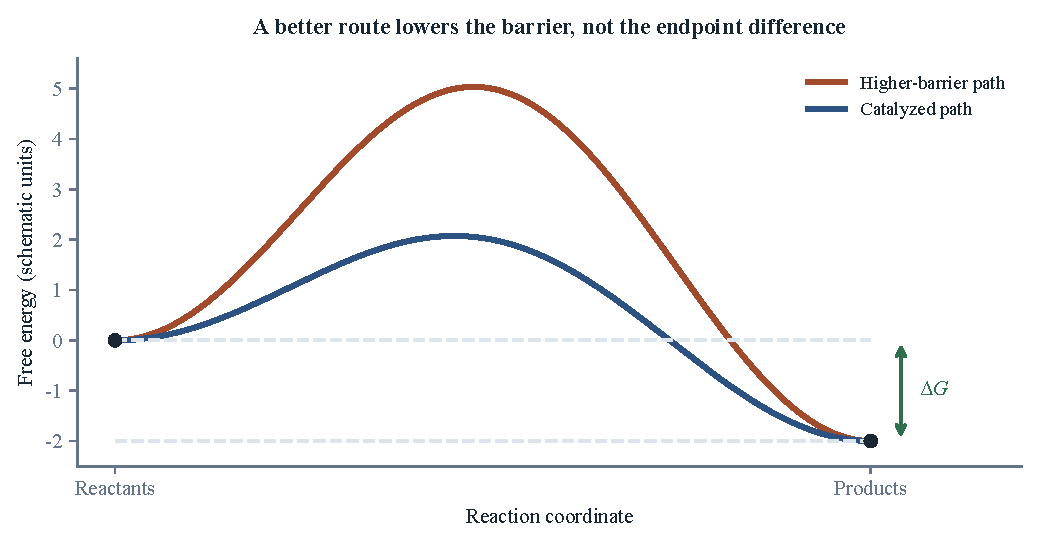
\includegraphics[width=\textwidth]{assets/activation-barrier.pdf}
\caption{A catalyst changes the route and its kinetic barrier. These schematic paths have identical endpoints and the same $\Delta G$. Lower activation free energy can accelerate reaction; the endpoint difference determines equilibrium.}
\label{fig:mechanism-activation-barrier}
\end{figure}
\subsection{The Weight of the Installed World}

\subhead{Past work made solid}

Cities contain accumulated extraction, processing, transport, lifting, assembly, finance, rules, and use. Roads and pipes occupy space and connect to occupied buildings. Their durability makes them useful and makes replacement a transition problem.

Research on global material stocks traces the huge accumulation of buildings and infrastructure during industrialization.\cite{krausmann2017global} Work on sediment flows likewise shows how extensively human activity moves and redirects material.\cite{syvitski2005impact} These stocks are a physical history with current users attached.

The work required to raise a mass through height $h$ in an approximately constant gravitational field is

\begin{equation}
W=mgh.
\end{equation}

For unchanged $m$ and $h$, a better drawing does not change this gravitational-energy difference. It can change the mass required, the construction route, or losses along that route. Lifting energy is one component of a building's account, often much smaller than the energy embodied in producing its materials.

The latest annual industry accounts keep the scale visible: world cement output is measured in billions of tonnes, and crude steel in roughly two billion tonnes.\cite{usgs2026cement,worldsteel2026figures} The relevant numbers are production flows, with stated years, not the full installed stock.

Replacing a district requires keeping services running, accommodating ownership, moving materials, and organizing a new configuration. A design can improve the destination while leaving the transition unaffordable. The installed world resists through the relations attached to its mass.

\subsection{Small Structures, Large Backends}

\subhead{Miniaturization changes the problem}

At smaller scales, mass becomes easier to move while defects, surface behavior, noise, tunneling, and heat become harder to manage. Semiconductor fabrication exposes the exchange. The product becomes small; the environment required to make it can become enormous.

The end of easy voltage and frequency scaling shifted more performance gains toward parallelism, specialized hardware, architecture, and packaging. “Dark silicon” describes a power-constrained gap between the transistors that fit on a chip and those that can operate at full activity together.\cite{esmaeilzadeh2011dark} Three-dimensional integration and other designs create new opportunities along with thermal and interconnect demands.

Thin barriers permit tunneling. Very small structures also turn discrete events into variability. Under a Poisson counting model,

\begin{equation}
\sigma_N=\sqrt N,\qquad \frac{\sigma_N}{N}=\frac{1}{\sqrt N}.
\end{equation}

To halve relative counting noise, four times as many events are required. Lithography has more mechanisms than photon counting alone, but stochastic exposure and resist behavior matter to defect control.\cite{debisschop2018stochastic} A nominal pattern and a reliably manufacturable pattern are different achievements.

\subhead{Heat has to leave}

A one-dimensional conductive approximation is

\begin{equation}
q''=\frac{P}{A}=-k_{\mathrm{th}}\frac{dT}{dx}.
\end{equation}

Heat flux density $q''$ has units W/m$^2$; $k_{\mathrm{th}}$ is conductivity. The sign follows the direction of decreasing temperature. Packaging adds interfaces, geometry, convection, and other heat paths. There is no universal air-cooling threshold for every device.

A facility repeats the problem at another scale. Concentrated computing needs power delivery and heat rejection. Better utilization and cooling can reduce demand per task.\cite{masanet2020recalibrating} Growth in tasks can still raise aggregate demand. In 2026, the IEA's account follows the network, supply, and connection constraints that accompany that growth.\cite{iea2026powering}

\subsection{Abundance, Concentration, and Recycling}

\subhead{Nature's inventory has a geography}

Primordial nucleosynthesis produced mostly hydrogen and helium. Later stellar and other nuclear processes produced heavier elements; planetary differentiation and geology redistributed them.\cite{steigman2007primordial,alpher1948origin,rudnick2003composition} A technical system inherits that distribution.

Abundance and availability diverge through concentration, location, chemistry, refining, equipment, and organization. For a mass fraction $\theta$, recovering a target mass $m$ requires at least

\begin{equation}
M=\frac{m}{\theta}
\end{equation}

of feedstock at perfect recovery. With recovery fraction $r<1$, the requirement becomes $m/(r\theta)$. Processing, energy, waste, and water demands depend on the actual ore and route, rather than only this inverse relation.

Critical-mineral studies follow the resulting concentrations in mining, refining, and supply chains.\cite{iea2021criticalminerals} Substitution can reduce dependence on one element while adding demands elsewhere. The useful question is which usable state the replacement requires.

\subhead{A second route through matter}

Recycling begins from a different initial state. Scrap aluminum already contains reduced metal; an ore route must perform reduction. Reuse can preserve even more of a component's fabrication history.

Collection, sorting, separation, purification, and requalification still have costs. Mixed materials, contamination, dispersion, and degradation can make a nominally recoverable stock difficult to use. The comparison is between routes, including their collection systems and the quality demanded of the result.

Across the scales, three obstacles recur: large stocks bind space and users; tiny structures magnify control demands; dispersed materials demand concentration. Intelligence can improve routes through all three. A useful route must still bring matter into the condition in which the function can exist.

\section{Temporal Rigidity: What Has to Unfold}

Compress a job's schedule and the loads do not automatically shrink with it. Energy, material, heat, inspection, and repair must pass through a shorter window. Speed becomes a demand placed on the receiving system.

\subsection{Time as a Flow Condition}

For an amount $\Delta X$ crossing area $A$ during interval $\Delta t$,

\begin{equation}
J=\frac{\Delta X}{A\Delta t}.
\label{eq:flux}
\end{equation}

The units depend on the quantity: mass flux, heat flux, and traffic flow describe different things. With amount and area fixed, shortening the interval increases flux density. More parallel capacity can change the area or number of channels; a new process can change the required amount.

A faster charging schedule can confront transport and reaction limits in a battery. Faster concrete placement can confront heat removal and temperature gradients. Faster manufacturing can outrun inspection or logistics. The proposed clock has to be supported by all the active paths.

Some delays are queues and can be removed by coordination. Others are transport times, reactions, growth, or exposures. A network can increase bandwidth without reducing signal propagation time along an unchanged route. A faster planner does not shorten a cable.

\subsection{Power, Heat, Stress, and Repair}

For fixed work,

\begin{equation}
P_{\mathrm{avg}}=\frac{\Delta W}{\Delta t},
\qquad
P_{\mathrm{avg}}\propto\frac{1}{\Delta t}.
\end{equation}

This accounting relation is exact. Whether required work stays fixed under acceleration is a separate physical question. Drag, losses, operating regimes, and the route itself can change.

Four constraints often move together. A supply must deliver the power. A thermal path must remove heat. Materials and joints must tolerate loading and cycles. Inspection and repair must contain faults before they propagate. Improving only the first can produce a hotter, more fragile process.

A faster production line illustrates the coupling. Reducing one station's cycle from 60 seconds to 45 seconds raises its nominal throughput by a third. Feeding, changeovers, quality control, packaging, and dispatch have to absorb the new output. Otherwise the gain becomes inventory between stations.

The right outcome measure is useful work completed at a specified quality and total cost. A high clock rate is one means of achieving it.

\subhead{Accelerated testing}

Engineering can exchange conditions for time. Higher temperature can accelerate some degradation mechanisms; higher cycling frequency can accumulate some forms of damage faster. An extrapolation works only where the accelerated process remains informative about the service process.

Change the mechanism and the test answers another question. This is why a faster test requires a model and validation of the acceleration factor. Better measurement can reveal an early signal, while an appropriate accelerated process can genuinely shorten the time required for evidence.

Likewise, prefabrication, controlled curing, different mixes, and thermal management can alter a construction schedule. “Twenty-eight days” names a familiar concrete strength benchmark, not a universal prohibition on earlier use. The process and acceptance conditions determine what the shorter schedule establishes.

\subsection{Updates and the Bandwidth of a System}

Shortening a process and sending it new instructions more often are different operations. A controller can receive frequent observations while holding an action stable long enough to evaluate its result.

A first-order response has the form

\begin{equation}
\tau\dot x+x=u(t),
\qquad
H(s)=\frac{1}{1+\tau s}.
\end{equation}

For a sinusoidal input,

\begin{equation}
|H(i\omega)|=\frac{1}{\sqrt{1+(\omega\tau)^2}},
\qquad
\arg H(i\omega)=-\arctan(\omega\tau).
\end{equation}

Higher-frequency inputs are attenuated and delayed. The model remains a stable low-pass response. An unstable closed loop requires an account of the controller, feedback signs, gain, delays, and actuator behavior.

Sampling faster can improve observation and control. Replanning faster can also amplify noise or repeatedly interrupt an action if the surrounding design lets it. These are design questions at the interface, not a general indictment of speed.

\subhead{Different layers, different clocks}

Electrical protection, local motor control, logistics planning, infrastructure replacement, and institutional learning run on different schedules. Fast fault isolation can be indispensable; constantly changing an organization's goals can make sustained work impossible.

The useful interface includes rate limits, buffers, holds, and hierarchy. A rate limit bounds how quickly an action changes. A buffer absorbs a fluctuation. A hold preserves a decision through an interval. Hierarchy keeps rapid local correction from repeatedly rewriting slow system objectives.

The interface also needs a record. If goals, models, instructions, and operating conditions all change between observations, learning what caused the outcome becomes difficult. A system can update constantly and complete very little.

\subsection{Biology and the Order of Events}

Life gives time another role. Gene expression, development, metabolism, immune response, repair, and adaptation occur in sequences with their own feedback. A prediction of the sequence and evidence about its actual course are different resources.

Drug development makes this visible. A candidate must reach the relevant tissue, act on its intended target, survive competing effects, and produce a useful outcome in people. Exposure and follow-up help establish what a short assay cannot.

The 2026 progress of rentosertib provides a current example. Insilico announced first patient dosing in its Phase III GENESIS-IPF-3 trial in September, following earlier clinical work. The planned 52-week treatment period is part of the study's attempt to establish efficacy and safety over a longer interval.\cite{insilico2026phase3} Advancing to that stage is a real achievement. Its result still comes from the study.

The same structure appears beyond medicine. Material fatigue emerges through loading history. An organization responds to rules, learns how to satisfy them, and sometimes finds ways around them. An ecological intervention propagates through relationships that extend beyond the first measured effect.

Four processes recur: accumulation, thresholds, adaptation, and propagation. Evidence has to follow the one responsible for the outcome. A single early measurement may be informative about a trend and inadequate to settle the final question.

\subsection{The Information Produced by a Process}

Some uncertainty can be reduced from information already available. Other uncertainty is reduced by allowing an intervention or an observation to occur. A field deployment produces information about contact with the field.

For $N$ strictly sequential physical stages, each requiring at least $\delta t$,

\begin{equation}
T\geq N\delta t.
\label{eq:steps}
\end{equation}

The statement is conditional on the chosen dependency chain and the lower bound on its stages. It does not prove that every complex process is computationally irreducible. A better algorithm may shortcut a calculation; a different process may change a physical dependency; parallelization may remove a previous bottleneck.

The valuable question is what the claimed shortcut changes. Does it produce the required exposure faster by a validated mechanism? Infer an outcome from a well-supported surrogate? Remove a dependency? Or merely stop observing earlier?

Early signals turn waiting into directed learning. A biomarker, a change in vibration, a developing crack, or a shift in behavior can justify intervention before a final failure occurs. Their value depends on the relation established between the signal and the outcome.

AI can improve candidate selection, experimental design, monitoring, and the interpretation of those signals. It can help spend a limited evidence budget on the most informative paths. A faster guess becomes a reliable gain when the connection to the required result is established.

The next constraint survives even that achievement. A verified component must still enter a system whose other parts already depend on one another. Time produces evidence; structure determines where the evidence can be used.

\section{Topological Rigidity: When Connections Become Weight}

A better destination can be easy to describe and difficult to reach. The difficulty may lie between the nodes: a component's dependencies, the order in which other parts must change, and the consequences of disturbing them.

\subsection{Coupling Density and Effective Mass}

\subhead{A goal needs a transition}

A hospital's new diagnostic system needs records, staff, laboratory processes, purchasing, review, and responsibility to work together. A faster port process can run into rail capacity outside the gate. A software module can be technically improved and incompatible with the accounting system that pays for its operation.

These connections give a small component a large transition cost. Its physical mass may be negligible while changing it requires many other parties to move. The book calls this \term{effective inertia}: a structural account of resistance, rather than a new quantity of mechanical mass.

For $N$ nodes, the maximum number of undirected pairwise links is

\begin{equation}
L_{\max}=\frac{N(N-1)}2.
\end{equation}

The count shows how many possible dependencies can exist. Real networks can remain sparse; links also differ in direction, strength, and function. A system's cost cannot be inferred from node count alone.

Network studies distinguish local structure, long-range paths, degree distributions, and the dynamics carried by the links.\cite{boccaletti2006complex,watts1998collective} Small-world work is especially useful for seeing how a few additional links can change distances without making every pair adjacent.\cite{milgram1967smallworld,travers1969experimental}

\subhead{An improvement absorbed by the system}

A local gain can be real and disappear from the aggregate result. Its output encounters another bottleneck, or its benefit is spent accommodating an existing dependency. A faster clinician's report may not change a patient's treatment date if imaging, specialist capacity, and follow-up remain binding.

The point is a diagnostic question: which relation converts the component gain into a service gain? A benchmark evaluates one part of that relation. Deployment evaluates the chain.

Technologies that change interfaces can therefore have effects larger than a component's nominal improvement. Containerization changed how ships, trucks, cranes, ports, and paperwork could connect; its effects depended on a network of complementary investments.\cite{bernhofen2016estimating} Standards can remove repeated translation work and make rearrangement easier.

They also establish a new installed base. A successful interface becomes something other parties expect to remain stable. An improvement produces a fresh history.

\subsection{Percolation and the Solidification of a Network}

\subhead{A local failure gains a route}

Percolation models examine when occupied sites or links form connected structures over large distances.\cite{broadbent1957,erdos1959} Below a threshold, disturbances may remain in small clusters. Above it, the same kind of local event may have a path across much of the system.

The threshold depends on the model and topology. A square lattice, a random graph, and a heterogeneous infrastructure network do not share one critical percentage. The useful question is what can now propagate.

The metaphor of \term{gelation} emphasizes a change in freedom of motion. Parts that once moved separately become constrained by a spanning web. In an organization, adding dependencies can make a change require coordinated movement. The resemblance helps formulate the mechanism; actual organizational coupling needs evidence about its links.

Interdependent networks can fail in cascades because one network's functioning nodes rely on the other.\cite{buldyrev2010} A local reliability score then misses a dependency failure. The distinction between random loss and targeted failure also matters in heterogeneous networks.\cite{albert2000error}

\subhead{Cascades with names and dates}

Historical infrastructure failures make the structure concrete. The 2003 North American blackout involved interacting equipment, operating conditions, awareness, and protection across a connected power system.\cite{uscanada2004} Treating each part's normal performance as an adequate description of the whole would omit the event.

The 2010 Flash Crash and Knight Capital's 2012 trading failure provide different financial mechanisms: rapid interaction among market behavior, automation, deployment, and controls.\cite{sec2010findings,sec2013knight} Their common feature is a fast propagation path. Their causes should not be collapsed into a single story about “too much intelligence.”

The 1999 Mars Climate Orbiter loss concerned an interface and unit mismatch within an organizational and technical process.\cite{nasa1999mishap} Aviation reviews of the 737 MAX likewise examine interacting design assumptions, human roles, integration, and certification rather than only the performance of an isolated function.\cite{jatr2019boeing}

These are historical cases. Their value is the failure mechanism documented in the investigation, not an implication that today's systems are unchanged.

\subhead{Why a pilot scales badly}

A pilot can select its users, concentrate expert attention, isolate a workflow, and provide exceptional support. Scaling reconnects what the pilot temporarily separated. Data formats, staffing, interfaces, maintenance, finance, and responsibility return at the boundary.

Simon called attention to nearly decomposable systems: strong local organization with more manageable interaction between subsystems.\cite{simon1962} Modularity can preserve a local failure boundary and let different parts evolve on different schedules.\cite{baldwin2000design}

An AI pilot that needs continuous exceptional care may be demonstrating the capability of a temporary organization, as well as a model. Scaling requires a repeatable organization for the surrounding work.

\subsection{Hysteresis and Structural Memory}

\subhead{History changes the next choice}

An installed road alters land use. A standard changes equipment purchases. A workflow shapes training and expectations. Later decisions begin from the world those decisions produced.

Path dependence describes how earlier choices alter later costs and options.\cite{david1985clio} Hysteresis describes a response that depends on the path taken, so reversing a control variable does not retrace the original state trajectory.

Material fatigue, magnetic hysteresis, organizational habits, and software dependencies have different mechanisms. In each, an adequate state description includes something carried forward from history.

\subhead{The freedom already committed}

An interface adopted by many organizations can freeze a choice into an obligation. Its continued use may be locally economical even when another arrangement would be better from a clean start. This is the difference between designing a new system and migrating a live one.

Compatibility can protect past investments. It can also preserve duplicated work and old limitations. Retiring the old route requires a plan for the parties whose functions depend on it.

Infrastructure studies examine the invisible installed base through which a new facility becomes usable.\cite{star1999layers} Conway's observation links software structure to communication within the organization that builds it.\cite{conway1968how} The code and the institution can carry the same history.

\subhead{What survives a change of scale}

Physics offers the language of coarse-graining: some microscopic variations disappear at a larger scale, while others remain relevant.\cite{wilson1971renormalization} The comparable organizational question is which local changes can affect the aggregate outcome.

A good tool can be absorbed by a procurement rule or a payment system. A new measurement can be absorbed by the incentives it creates. Measures used to allocate rewards invite the responses discussed by Goodhart and Campbell.\cite{goodhart1975problems,campbell1979assessing}

A removed tool also leaves effects. Users have learned, data have moved, expectations have changed, and contracts have been signed. A rollback plan must specify which state it can recover. Restoring software may leave the surrounding consequences untouched.

\subhead{Making history editable}

A transition architecture includes compatibility, parallel operation, staged cutovers, migration of records, and a credible retirement point. Without retirement, each improvement can become one more permanent layer.

Banking migrations demonstrate the stakes of cutover and service continuity. The TSB migration and regulatory investigation document a transition failure with consequences for access, customers, and operations.\cite{tsb2019migration} A payment process also depends on settlement and trust arrangements beyond the speed of its message.\cite{kahn2009why}

The objective is to make an installed system changeable while it remains in use. That is a capability of the structure.

\subsection{Reachability and the Equilibrium People Choose}

\subhead{Possible is larger than reachable}

A generated plan describes a destination. A reachable destination requires a permitted path from the current state, the resources and time to take it, and conditions under which the result can persist.

There can be many physically feasible paths and a narrow set of socially maintained ones. People respond to prices, rules, expectations, and one another. The equilibrium reached through their choices may be poor even when a better feasible arrangement exists.

Wardrop's traffic framework and work on the cost of uncoordinated routing formalize this distinction in a defined setting.\cite{wardrop1952some,roughgarden2002how} Adding a path expands the feasible set, yet independent users can move to a worse equilibrium. The available capacity and the way it is used require separate analysis.

Road construction can also change demand. Evidence on induced travel examines a further response beyond fixed-demand routing.\cite{duranton2011fundamental} More attractive supply can draw additional use into the system.

\subhead{The option that survives collective use}

AI expands the supply of strategies, recommendations, and entry points. A strategy's effect at low adoption may differ from its effect when many agents use it. A market signal can crowd a trade; a common recommendation can crowd a route; a generated workflow can crowd a shared reviewer.

Evaluating this outcome requires a model of the users' response. The number of alternatives generated is not a measure of the alternatives that remain serviceable under simultaneous use.

Governance can change those responses through pricing, scheduling, access rules, and coordination. The desired state needs a route and an arrangement that keeps it viable.

\subhead{Slack and plasticity}

High utilization can make a normal period look efficient while leaving few options when conditions change. Alternative suppliers, buffers, repair capacity, and isolation can preserve useful routes under disturbance.

Work on highly optimized tolerance describes systems that are efficient for anticipated conditions and vulnerable outside them.\cite{carlson1999highly} Robustness has a distribution: strong protection in one direction can coexist with a weakness in another.

\term{Plasticity} is the capacity to change structure while maintaining enough function to continue. Too little coupling prevents cooperation; too much compulsory coupling prevents adaptation. A durable system needs both useful commitments and places where commitments can be revised.

\subsection{Dependency Surface, Synchronization, and Rollback}

\subhead{Three sources of effective inertia}

The \term{dependency surface} asks how many relationships a change touches, and how consequential those relationships are. The \term{synchronization cost} asks which of them must move together. The \term{rollback cost} asks what can be recovered after failure.

A personal script may have a small dependency surface. A module connected to payroll, inventory, invoicing, compliance, and customer access has a larger one. A compatible update can permit gradual migration; a format change that every participant must adopt at once creates a coordination problem.

Splitting software into services can isolate work and support independent change. It can also introduce distributed state, observability, versioning, and operational dependencies. Research on microservice migration records such tradeoffs.\cite{taibi2018architectural} The number of modules alone measures neither freedom nor complexity.

\subhead{The external links}

Power and logistics show how dependencies extend beyond one operator. A fuel interruption can affect electricity supply; transport policies and routes influence what can arrive; a blocked canal can redistribute shipping flows.\cite{morison2004power,nzmfat2021,suez2021} These cases require different explanations, while revealing a common need to trace the links outside an organization's diagram.

Recent work on operational systems likewise treats deployment as an interaction among tools, operators, and the processes surrounding them.\cite{dong2022operational} The question for an AI application is where it sits within that structure.

A modest tool with a small dependency surface may spread rapidly. A more capable tool at a critical interface may remain difficult to deploy. Matching intelligence to a structure requires an input boundary, an output boundary, a failure plan, and a responsible operator.

Connections produce both capability and weight. The engineering task is to keep the former while making the latter manageable.

\section{The R--T--G Framework}

Resources, process time, and dependencies describe different conditions of a transition. Fix the task, outcome, accounting boundary, and horizon before comparing them. Otherwise a cheap first attempt can be mistaken for a cheap completed result.

\subhead{Coordinates and a response}

Let $(R,T,G)$ describe resource barriers, temporal rigidity, and topological coupling. Let $\eta$ measure the transition cost relative to a stated reference:

\begin{equation}
\eta=f(R,T,G).
\label{eq:eta-rtg}
\end{equation}

The coordinates describe sources of difficulty; $\eta$ is a response to be observed. Their units and normalization depend on the operational definitions.

A working model is

\begin{equation}
\eta=\eta_0\exp(\alpha R+\beta T+\gamma G).
\label{eq:eta-exp}
\end{equation}

Here $\eta_0$ is a reference value. The exponent must be dimensionless. With normalized coordinates, the coefficients describe marginal changes in log-cost over the range being studied. Interactions and changing coefficients can be added when the data justify them.

\begin{table}[ht]
\centering
\caption{Three coordinates, three deployment questions}
\label{tab:ch2-rtg}
{\small
\begin{tabularx}{\textwidth}{@{}lYYY@{}}
\toprule
 & Question & Typical evidence & What an intervention may change\\
\midrule
$R$ & Can the change be supplied? & Material, energy, equipment, capital & Resource use, capacity, maintenance\\
$T$ & Can the process fit the window? & Dependencies, exposure, testing, coordination & Critical path, parallel work, risk\\
$G$ & Can the connected system absorb it? & Interfaces, synchronization, recovery & Isolation, migration, accountability\\
\bottomrule
\end{tabularx}}
\end{table}

More equipment may relieve a deadline and increase capital cost. Standardization may reduce both coordination effort and waste. A safety process may add time while reducing later losses. Those directions are measured outcomes, rather than rules requiring every saving to be charged elsewhere.

\subhead{Tradeoffs have a feasible set}

At constant $\eta$, with coefficients held fixed,

\begin{equation}
\alpha\,dR+\beta\,dT+\gamma\,dG=0,
\qquad
\left.\frac{dR}{dT}\right|_{\eta,G}=-\frac{\beta}{\alpha}.
\end{equation}

The relation describes an iso-cost surface of the model. A real process can move along it only where a feasible engineering or institutional route exists. Different normalizations change the coefficient ratios; different tasks can change the model.

This distinction prevents a common misuse: a mathematical compensation is not a purchasable substitution. A larger budget cannot always buy the required exposure period. A long schedule cannot supply a missing element. A new interface can sometimes remove a synchronization requirement that was previously expensive.

\subhead{Thermodynamic limits}

For a closed reaction system coupled to a reservoir at fixed temperature $T_0$ and pressure $p_0$, with the stated initial and final states, the reversible minimum net non-volume work input is

\begin{equation}
W_{\min}=\Delta G=G_{\mathrm f}-G_{\mathrm i}.
\end{equation}

Under the corresponding boundary and exchange assumptions, irreversibility adds a term related to entropy production:

\begin{equation}
W_{\mathrm{in}}=\Delta G+T_0S_{\mathrm{gen}},
\qquad S_{\mathrm{gen}}\geq0.
\end{equation}

Other heat exchanges, material flows, or constraints require the appropriate exergy account. A theoretical minimum and a plant's actual total consumption answer different questions.

Aluminum makes the initial-state issue visible. Producing metal from alumina and remelting suitable aluminum scrap start from different states. The latter retains part of the work performed earlier and can therefore require much less energy.\cite{quinkertz2001scenario} Calling one route more intelligent cannot explain the difference by itself.

\subhead{Structural bookkeeping}

With a consistent complexity measure and boundary,

\begin{equation}
\Delta C_{\mathrm{tot}}=
\Delta C_{\mathrm{local}}+\Delta C_{\mathrm{rest}}.
\end{equation}

The identity tracks redistribution. Total complexity can rise, stay constant, or fall. Removing redundant interfaces can reduce it; automating one operation while building a large support system can increase it.

The same separation applies to risk and responsibility. A local operator's workload may fall while a customer or another institution inherits the difficult remainder. The total and its allocation belong in different columns of the account.

\subhead{How to use the framework}

Fusion provides a demanding resource-and-time combination. A representative deuterium-tritium criterion is commonly expressed through density, temperature, and energy-confinement time:

\begin{equation}
nT\tau_E\gtrsim
3\times10^{21}\ \mathrm{keV\,s\,m^{-3}},
\end{equation}

for stated plasma assumptions near the relevant operating region.\cite{lawson1957some} The exact threshold depends on the criterion and regime. A power plant must also close its engineering and economic balances.

At another extreme, a generated draft can appear cheaply and quickly while its use remains blocked by evidence or authorization. In one case the apparatus and physical process dominate; in the other, generation can be easy and the receiving interface difficult.

The framework directs attention to the bottleneck and to the proposed intervention's actual effect. It is used qualitatively with explicit criteria where calibration is unavailable. Quantitative prediction needs defined variables, fitted coefficients, uncertainty, and tests against alternatives. The appendix develops that route.

The next chapter follows the transition itself. Once intelligence reaches an interface, what does the medium do with the input?

\chapter{Intelligence at the Interface}

The previous chapter described resistance. This chapter follows the disturbance that meets it. When a model begins to send commands, allocate work, or initiate actions, its outputs become inputs to a system with dynamics of its own.

A sentence can be evaluated as a sentence. A command must also be evaluated through the movement, load, feedback, and consequences it produces. The interface changes the task.

\section{From Solver to Driver}

\subsection{A Different Position in the Loop}

\subhead{A solution that has to act}

A solver compares possibilities and returns a candidate. A driver participates in changing the state of the world. It sends a signal through an actuator or an organization, observes a result, and helps determine the next action.

The phrase “phase change” describes this shift in role. The new system is evaluated on whether the transition occurs, remains stable, and can be recovered from when it goes wrong.

Ashby's law of requisite variety gives an early account of why the shift matters.\cite{ashby1956cybernetics} A regulator needs enough available distinctions and responses to counter the disturbances relevant to its task. Many words about a disturbance do not necessarily supply an actuator that can correct it.

A robot may describe a dropped object without being able to reach it in time. A logistics system may identify a delay without having a spare vehicle. Control authority has to exist at the location and time where the correction is needed.

\subhead{The answer becomes part of a cycle}

In a closed loop, the sequence is observation, decision, action, response, and a new observation. Each has latency and error. The model acts on an estimate of a state that may already have changed.

Wiener's work grew from precisely such prediction-and-action problems.\cite{wiener1948} Modern control theory evaluates a controller together with the plant, sensing, delay, and disturbance.\cite{astrom2008} The quality of a stand-alone forecast is one part of the result.

Supply-chain experiments show how people can also destabilize delayed feedback through their ordering decisions.\cite{sterman1989,lee1997} A system that reacts vigorously to a lagging signal can amplify the condition it is trying to correct.

Faster observation and computation can improve control. Their effect depends on the loop into which they enter. The gain has to be placed where the receiving process can use it.

\subsection{Four Conditions of Executability}

\subhead{Power, bandwidth, error, and safety}

An executable plan must fit four kinds of constraint.

First, the action needs adequate power and force at the relevant scale. Second, the receiving medium must be able to respond over the required bandwidth. Third, estimation, prediction, and execution errors must remain within the task's tolerances. Fourth, the failure modes must fit a defensible safety arrangement.

These conditions interact. A lighter actuator may move faster and tolerate less load. A higher gain may improve nominal tracking and excite an unmodeled mode. More sensors can improve observability while adding communications and maintenance requirements.

Safety engineering examines the interaction among components, people, organizations, and operating conditions.\cite{perrow1984,leveson2011} A component's success rate cannot establish the safety of every system into which it can be connected.

\subhead{Why the chosen path bends}

A shortest route on a map can have poor traction, a closed gate, an unsafe crossing, or an inaccessible entrance. A nominally optimal manufacturing schedule can eliminate the time needed for cleaning or repair. The path bends around conditions omitted from the first optimization.

The useful objective becomes a route that can be sustained at an acceptable total cost. It can include redundancy, staged release, human review, or spare capacity. These are design variables with measurable functions.

The receiving organization matters as much as the actuator. A clinical recommendation must enter a workflow with the information, authority, staffing, and follow-up necessary to act on it. An instruction no one can safely carry out remains an instruction.

\subhead{Embodiment as integration}

Brooks and later work on embodiment emphasized that useful behavior depends on the coupled body and environment.\cite{brooks1991,pfeifer2006} Sensors, morphology, compliance, feedback, and physical contact can perform work that a detached planner would otherwise have to specify.

Vision-language-action models extend this integration. RT-2 connected web-scale visual and language representations with robot action data.\cite{zitkovich2023} Its significance is the attempt to carry knowledge into action, where trajectories and outcomes impose another test.

Contemporary deployment shows the surrounding work. GXO's October 26, 2026 announcement expanded its relationship with Agility Robotics from an earlier live warehouse deployment and described planned additional sites.\cite{gxo2026digit} The relevant unit of progress is a robot within a workflow, with material handoffs, uptime, service, and supervision attached.

Autonomous-driving validation studies similarly examine the distance between observed operation and a sufficiently strong safety claim.\cite{kalra2016,koopman2016} Rare events, scenario coverage, operational limits, and the evidence supporting a release all matter.

A usable driver is an arrangement of model, body or tools, environment, and organization. Its capability is distributed across that arrangement.

\section{How a Medium Absorbs Intelligence}

The same output rate can mean abundance in one setting and overload in another. The difference lies in what must happen after the output arrives.

\subsection{Three Response Patterns}

\subhead{Bits: diffusion and replication}

Digital output can be copied and transmitted with little additional handling per recipient. A patch, image, or document can therefore spread rapidly. Once it enters a shared state, a production process, or a decision, its failure costs change.

Digital traffic can also outrun a channel. Congestion-control work treats the network's capacity and feedback as part of the sending problem.\cite{jacobson1988} A sender that can create more packets has not established that more packets will arrive usefully.

Generated material introduces an evidential version of the same issue. More records can make source tracking and quality control harder. Research on recursive training with generated data identifies conditions under which a distribution can deteriorate; it does not establish that every use of synthetic data must fail.\cite{shumailov2024ai}

\subhead{Atoms: work and sequential operations}

A manufactured output has to pass through actual operations. Some are parallelizable, others form a critical path. Adding plans does not automatically add machines, crews, feedstock, or a heat-removal path.

A production line can respond with an initial delay followed by a limited rate of output. Once a demand fits its capacity, a more intelligent schedule can help. Above capacity, priorities, queues, rejection, and investment determine what happens next.

\subhead{Life: response to an intervention}

A living system responds through regulation, compensation, adaptation, and multiple timescales. A dose changes concentrations, which change interactions, which can alter the subsequent response. The action enters a system already maintaining itself.

Shear thickening in suspensions provides a physical image of resistance that can rise with the rate of imposed deformation.\cite{brown2014shear} Biological and social resistance need their own mechanisms and measurements. The image directs attention toward a rate-dependent response.

Three elementary curves illustrate possible response shapes:

\begin{align}
y_b(t)&=y_\infty(1-e^{-t/\tau_b}),\label{eq:resp-bit}\\
y_a(t)&=y_\infty\min\left\{\frac{(t-t_d)_+}{\tau_a},1\right\},\label{eq:resp-atom}\\
y_l(t)&=y_\infty\left[1-e^{-\zeta\omega_n t}
\left(\cos\omega_dt+\frac{\zeta}{\sqrt{1-\zeta^2}}\sin\omega_dt\right)\right],
\label{eq:resp-life}
\end{align}

where $\omega_d=\omega_n\sqrt{1-\zeta^2}$ and $0<\zeta<1$ for the third curve. The first is a first-order approach, the second a delayed rate-limited completion, and the third an underdamped second-order response.

They are worked examples, with parameters to be fitted for a chosen process. A digital migration can be slow, a physical relay very fast, and a biological response overdamped. The medium suggests questions about the mechanism; it does not assign the curve.

\subsection{Mismatch at the Interface}

\subhead{A useful signal needs a receiving capacity}

Electrical engineering gives a precise case of mismatch. For a lossless line of real positive characteristic impedance $Z_0$ terminated by a load $Z_L$,

\begin{equation}
\Gamma=\frac{Z_L-Z_0}{Z_L+Z_0},
\qquad
\frac{P_{\mathrm{refl}}}{P_{\mathrm{in}}}=|\Gamma|^2.
\end{equation}

Matching removes reflection under the stated conditions. An AI interface has different variables, so its wasted outputs cannot simply be assigned this electrical coefficient. Their measurable forms include discarded work, waiting, repeated replanning, and damage.

Let $r=v_{\mathrm{in}}/v_{\mathrm{abs}}$ compare an arrival rate with absorption capacity in the same units. An illustrative effective-progress response is

\begin{equation}
u(r)=
\begin{cases}
r,&0\leq r\leq1,\\
1-\kappa(r-1)^m,&r>1,
\end{cases}
\qquad \kappa>0,\quad m>0.
\label{eq:rate-mismatch}
\end{equation}

Below capacity, added input can increase progress. Above it, an overload penalty can offset the gain and, if damage is included in net progress, make it negative. The curve proposes a response to test. A pure queue with no damage instead produces waiting and a saturated service rate.

\subhead{Fit the interface to the task}

The practical choices are selective admission, buffering, a stable command interval, parallel receiving capacity, and a route for feedback. Their value depends on the process.

A contact controller needs fast local sensing and correction. A high-level language model can choose a task while a local policy maintains a grip. A laboratory system can generate candidates freely while admitting only a funded and informative selection to experiments.

The interface decides how intelligence becomes load. Designing it is part of building an intelligent system.

\begin{figure}[ht]
\centering
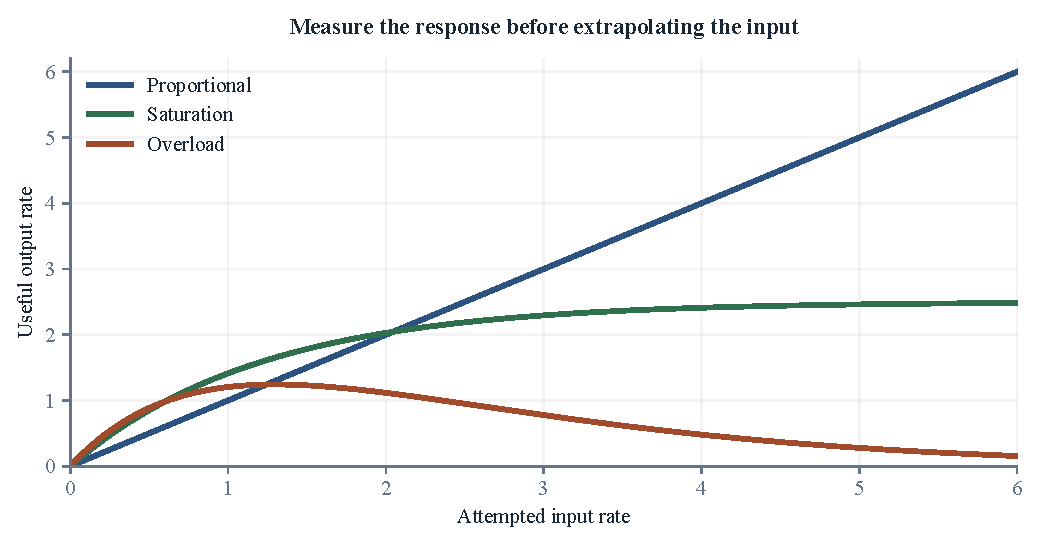
\includegraphics[width=\textwidth]{assets/response-regimes.pdf}
\caption{Useful output can scale with input, saturate, or fall under overload. These are illustrative response forms; measurements determine the form and parameters of a particular system.}
\label{fig:mechanism-response-regimes}
\end{figure}

\section{Overlays and the Complexity Ratchet}

\subsection{Why New Systems Grow on Old Ones}

\subhead{Three bills for reconstruction}

Replacing a live system presents three bills. Its material assets have to be changed. Service has to continue through the transition. Its participants have to coordinate around new rules and interfaces.

An overlay can avoid paying all three immediately. Navigation uses existing roads. A hospital assistant uses existing records and staff. A sensor layer observes an existing factory. New capability attaches to the installed base.

The strategy is often rational. Its apparent lightness can conceal work needed to translate between layers, maintain consistency, and recover when the overlay fails.

\subhead{The price of leaving the environment alone}

Moravec's contrast between formal intellectual tasks and everyday sensorimotor competence helps explain why a computer-centered route initially spreads unevenly.\cite{moravec1988} Standardizing a task can remove difficulties that a more general machine would have to handle.

Autonomous driving takes one version of the choice. A heavily controlled route can simplify operation; public mixed traffic requires the vehicle and service to accommodate a much larger range of conditions. Evidence about operational safety has to match the chosen domain.\cite{kalra2016}

The vehicle carries some complexity because the surrounding world remains available to many kinds of user. This can be a good social and engineering choice. Its costs belong in the vehicle, operating service, and governance account.

\subsection{What Accumulates Between Layers}

\subhead{A model of a ratchet}

Suppose adding a layer contributes $c$ units of maintenance complexity and causes existing complexity to grow by fraction $\alpha$:

\begin{equation}
C_{n+1}=(1+\alpha)C_n+c.
\label{eq:ratchet-recursion}
\end{equation}

For constant $\alpha>0$,

\begin{equation}
C_n=(1+\alpha)^nC_0+
\frac{c}{\alpha}\big[(1+\alpha)^n-1\big].
\label{eq:ratchet-floor}
\end{equation}

For $\alpha=0$, the result is $C_0+nc$. Positive proportional interaction produces exponential growth in this model. Real systems can consolidate, standardize, retire components, and remove dependencies; their growth need not follow the recurrence.

The ratchet appears when removing a layer leaves obligations behind. Upstream systems now expect its data; downstream workers expect its decisions; exception procedures depend on its presence. Another arrangement must assume those functions before removal is complete.

A residual model $C_n^{\mathrm{res}}=\beta_n C_n$ records a fraction that remains after a specified removal, with $\beta_n$ to be measured. It is a description of the chosen transition, rather than a universal lower bound.

\subhead{Compatibility and deployment costs}

Compatibility work preserves relations between versions, formats, interfaces, and operating practices. Deployment work establishes a service in actual use: integration, testing, monitoring, support, incident response, and responsibility.

Under a particular additive removal protocol, one may define an index

\begin{equation}
K_n=\sum_{k=1}^n\big(C_k-C_k^{\mathrm{res}}\big).
\label{eq:compat-tax}
\end{equation}

Counting this as labor or money requires cost weights and a check that the same work is not counted twice. The useful empirical question is how much work it takes to release the dependencies, not how large an index can be made.

An overlay earns its place when its total benefit exceeds these costs. Its risk is institutional permanence by default: each new layer is temporary until someone asks what removal would require.

\subhead{Designing an exit}

A credible overlay has an exit condition. It may be retired after a migration, consolidated into a stable module, or replaced by a simpler underlying process. Parallel operation should have a purpose and a horizon.

Some interfaces deserve long lives. Others continue because no one owns the cleanup. The complexity ratchet is strongest where benefit belongs to the builder and maintenance belongs to someone else.

The next section follows what happens when input keeps arriving faster than the system can be rebuilt.

\section{What the System Does with More Intelligence}

An input does not acquire priority because it came from an intelligent machine. Once it enters a factory, a market, or an organization, the receiving system decides what happens next. Some inputs find a better route. Some accumulate. Some help drive the system unstable. These are different mechanisms, and they require different remedies.

\subsection{Rerouting: Moving Some of the Trial and Error}

The direct route is often the expensive route. A desired molecule is easy to describe and hard to synthesize. A production target is easy to enter into a spreadsheet and hard to reach with the equipment already installed. A search algorithm earns its keep when it discovers a path that asks less of the costly medium.

Call this a \emph{probabilistic shortcut}: spend computation to improve the odds of the next expensive intervention. Screen candidate compounds before synthesizing them. Simulate a warehouse layout before moving the racks. Search a design space before cutting metal. The saving comes from changing which physical trials are attempted, how they are ordered, and how much each trial teaches.

Monte Carlo methods made a related trade long before deep learning. Sampling replaces certain difficult calculations with estimates whose precision depends on the sampling scheme and budget. It does not make every estimate cheap or every rare event visible. It gives engineers a different way to buy an answer. In games, systems such as AlphaGo could search within rules that were already executable, with outcomes that could be obtained without building a physical board or waiting for a human opponent \cite{silver2016mastering}. The search environment supplied an unusually inexpensive judge.

The judge becomes more costly outside games. A predicted protein structure may narrow an experiment, suggest a mechanism, or support a screening workflow. The experimental question then matters: determining a structure, establishing binding, measuring activity, and demonstrating a therapeutic benefit are different tasks. A prediction need not be remeasured in every downstream use to be useful, but its uncertainty must be compatible with that use. Cheap structure proposals do not turn every biological claim into an established result.

Semiconductor fabrication illustrates another form of rerouting. When a direct scaling path becomes difficult, progress can continue through new materials, transistor structures, packaging, architecture, and specialized computation. Each route changes the cost distribution. More elaborate fabrication may buy performance at the price of more process steps, tighter tolerances, and expensive equipment. The result can be a real improvement without being a disappearance of resistance.

The same test applies to simulation. A simulator can fail a thousand times without breaking a gripper. Yet someone must establish which failures and successes transfer to the actual gripper. Domain randomization can improve transfer by exposing a policy to varied conditions; the range of variation remains a modeling decision \cite{tobin2017domain}. A shortcut pays when the physical trials it avoids cost more than the computation, modeling, and additional uncertainty it introduces.

The useful question is therefore concrete: \emph{which part of the real trial has been removed, which part has been moved, and which part still has to happen?} A project that cannot answer this may have relocated its bottleneck while mistaking the relocation for a breakthrough.

\subsection{Accumulation: Intelligence Becomes Inventory}

Consider an engineering team whose assistants can generate a hundred plausible patches a day. Its reviewers can investigate ten. Its test infrastructure can run more tests than before, but production incidents still require experienced staff. The organization now has a larger candidate inventory. Whether it has more reliable software depends on the receiving process.

For a queue with arrival rate $I(t)$ and absorption rate $A(S)$,
\begin{equation}
 \frac{\mathrm{d}S}{\mathrm{d}t}=I(t)-A(S),
 \qquad 0\leq A(S)\leq A_{\max}.
\end{equation}
$S$ counts unfinished items. The rates count items per unit time. At an empty queue, departures cannot exceed available work; a more detailed model would also include rejection, abandonment, rework, and different classes of item. The accounting point survives: sustained arrivals above effective service capacity create a growing backlog.

A backlog is stored time. It can be useful. Hospitals hold spare supplies, cloud systems buffer bursts, and laboratories retain promising candidates until an instrument becomes available. Inventory becomes a problem when it conceals an absorption limit. A long list of unreviewed proposals may look like a rich pipeline while making urgent work harder to identify.

Even stable queues can have long delays when utilization is high and arrivals or service times vary. Spare capacity buys something that an average throughput chart can hide: the ability to absorb a surprise. Running every expert, machine, and approval channel at nominal capacity leaves little room to recover from an exception.

Accumulation also moves upstream. If an experimental facility is booked months ahead, researchers change what they propose. If deployment review becomes the bottleneck, developers optimize for the review process. The downstream constraint starts shaping the supposedly unconstrained search space.

Supply chains show how this can become oscillation. Demand signals pass through ordering policies, inventory targets, production schedules, and delivery delays. Local adjustments can amplify a small change in final demand into much larger upstream orders: the bullwhip effect \cite{lee1997information}. Better information can help, but information alone does not remove lead times or correct a badly tuned replenishment rule.

There is no universal clock assigning short cycles to light assets and long cycles to heavy ones. Nevertheless, adjustment times matter. Clearing a content queue and rebuilding a power plant operate on different clocks. A decision that was appropriate when initiated may reach completion in a changed environment. Heavy commitments preserve old expectations in physical form.

Reducing arrivals can relieve a queue; increasing service capacity can raise its sustainable throughput. Improving candidate quality can do both by reducing rework and increasing the useful output of each review. These are distinct interventions. Generating more candidates addresses none of them by itself.

\subsection{Instability: Correction Becomes a Disturbance}

Oscillation is not the inevitable outcome of fast computation. A well-designed controller can use rapid measurements to stabilize a slow plant. The danger is a control policy whose gain, delay, and model do not fit the plant it is controlling.

An operator sees a shortfall and orders more capacity. Before the capacity arrives, the shortfall persists, so the operator orders still more. When the first expansion comes online, the later orders remain in motion. The controller has interpreted the absence of an immediate response as evidence that its previous action was too weak.

This is how a sensible local instruction can create a damaging global rhythm. A warehouse keeps rerouting staff before any team has settled into its new task. A company changes quarterly objectives before the previous reorganization has produced interpretable evidence. An automated market strategy reacts to liquidity that disappears as other strategies react to it.

The official investigation of the May 2010 US market disruption documented interactions among a large sell program, changing liquidity, and trading behavior \cite{sec2010findings}. It is a historical case of interacting mechanisms, rather than proof that trading speed alone causes crashes. A fast system needs an account of what its own action does to the signals it will read next.

Protective devices enter that same loop. A trading halt can create time for liquidity and information to recover. A known threshold can also alter behavior before the halt: participants may trade earlier because they expect access to close. Theoretical work on price limits describes such a magnet effect \cite{subrahmanyam1994}. A threshold must be evaluated with the behavior it induces.

In physical control, inertia, damping, and active compensation have distinct roles. Inertia slows a change in velocity or frequency; damping dissipates an oscillation; a controller can supply a response that depends on its design and available energy. Calling all three “friction” obscures the engineering. Their common relevance here is that rapid decisions need a receiving system capable of turning them into a stable trajectory.

Three questions separate the interventions. Can search identify a route that needs fewer costly trials? Can the receiving process absorb the proposed work? Does the feedback policy remain stable with actual delays and disturbances? The corresponding investments are better validation, better absorption, and better control.

More intelligence can improve all three. It can also flood a review queue, accelerate a badly chosen intervention, or exploit a shortcut that works only inside the model. The difference lies in what becomes of the input after it crosses the interface.

\section{When a Generated Answer Becomes a Result}

A fabricated reference can have a convincing title, plausible authors, and the right journal style. An invalid proof can have lemmas, notation, and impeccable transitions. A patch can look clean while calling an interface that does not exist. In each case, the output possesses a recognizable form. What it lacks is a completed route from that form to a dependable result.

Language models have made this separation industrially important. Candidate production can run ahead of candidate confirmation. The question is no longer simply where an answer came from. It is what has established the answer, at which level, and for which use.

\subsection{The Two Jobs of Form}

Form is a transferable constraint. A proof rule limits which steps may follow. A function signature limits which calls are well formed. A narrative structure limits what a reader expects next. Their constraints differ in strength and purpose, but each allows something learned in one setting to carry into another.

Formal logic isolates an especially powerful case. A valid inference preserves its validity when suitable contents are substituted into its structure. The achievement is compression: one rule can govern indefinitely many instances. The rule does not need to retain every instance separately.

The history from axiomatized geometry to symbolic logic made this power explicit. It also raised a harder ambition: could a sufficiently complete formal system settle every question in its domain and establish its own reliability from within?

The limits have precise statements. A consistent, effectively axiomatized theory strong enough for elementary arithmetic is incomplete. Under the usual conditions of the second incompleteness theorem, it cannot prove its own formalized consistency \cite{godel1931}. The halting problem rules out one algorithm deciding whether every arbitrary program halts \cite{turing1936}. Algorithmic information theory establishes that some finite strings have no substantially shorter description in a chosen universal description language \cite{chaitin1987}.

These results concern different objects. They do not show that every particular proof needs an unprovable assumption, that every program is beyond analysis, or that fluent language is inherently unreliable. What they prohibit are specific forms of universal closure. Engineers still prove particular properties of particular programs, using explicit assumptions and a specified logic.

Deployment adds a separate boundary: the correspondence between the formal object and the thing being built. A verified controller can satisfy a specification whose sensor model is wrong. A correct compiler can preserve the semantics of a program that expresses the wrong requirement. A sound proof checker can accept a theorem that is weaker than the informal claim used to advertise it.

The seL4 verification demonstrated a machine-checked refinement from an abstract specification to a C implementation, with explicit assumptions and exclusions \cite{klein2009sel4}. CompCert established semantic preservation for a substantial compiler, again within a defined account of source and target behavior \cite{leroy2009compcert}. These achievements make the boundary inspectable. They also show the work involved in connecting a claim to an implementation.

A result is valuable partly because one can say exactly what was established. “Verified” without the property, assumptions, and implementation boundary leaves the central question unanswered.

\subsection{How Prediction Learns Structure}

Earlier symbolic systems relied heavily on people writing rules. Learned models obtain much of their structure from records: language, code, diagrams, demonstrations, experimental reports, and the traces of other people's reasoning.

These records are highly patterned. Variable binding, references, function calls, nested expressions, and relations between goals and actions reduce uncertainty across many contexts. A model that represents such regularities can predict better than one that memorizes isolated fragments. Prediction can therefore create an incentive to learn useful abstract structure. Which structures it learns, and how reliably it uses them, remain empirical questions.

The physical process matters too. Training consumes electricity, moves data, changes stored states, and rejects heat. For an idealized reset of an unbiased bit, coupled to a thermal environment at temperature $T$, Landauer's bound is
\begin{equation}
 Q_{\min}=k_{\mathrm B}T\ln 2.
\end{equation}
At about $300\,\mathrm{K}$ this is roughly $2.9\times10^{-21}\,\mathrm{J}$ per bit reset. The bound concerns logically irreversible information erasure under the stated conditions; it is not a universal invoice attached to every arithmetic operation or memory write. Real hardware operates with additional device, communication, memory, and cooling costs.

Energy permits the computation. Structured data supplies learnable regularity. The objective and optimization process favor some representations over others. These roles cannot be collapsed into the claim that dissipation produces intelligence. A resistor dissipates energy without learning a grammar.

One can picture training as carving channels through a landscape: repeated data and error signals make some continuations easier than others. The image explains why widely recurring structures may become accessible together. It supplies no theorem that the resulting channels track truth.

The training objective rewards an operational target. In a prediction task, that target is predictive performance on a distribution of records. A true statement can be surprising in that distribution. A false statement can be conventional. A model can learn useful reasoning procedures and still apply them incorrectly to a particular case.

The GPT-4 technical report is a historical example of this coexistence: substantial capability accompanied by factual and reasoning failures \cite{openai2023gpt4}. It is evidence about a particular generation of systems, rather than a current frontier benchmark. The general engineering question persists as systems improve: what evidence connects this output to the object, rule, or environment on which it makes a claim?

Hallucinations have multiple sources, including data quality, objectives, retrieval failures, decoding, and reasoning errors \cite{huang2023hallucination}. Treating them as a single irreducible price of creativity would overstate the case. Individual error classes can be reduced, detected, or excluded by design. The harder problem is establishing reliability across the full range of uses advertised for a system.

\subsection{Three Places Where Confirmation Happens}

A bibliographic reference needs an identifiable source. A mathematical derivation needs valid inference. A warehouse plan needs an executable and acceptable intervention. These are three useful places to inspect a confirmation chain.

\begin{enumerate}
 \item \textbf{Reference.} Does the representation point to the claimed object? A paper title, API name, data field, or quoted finding must be traceable to something that supports its use.
 \item \textbf{Inference and execution.} Do the transformations obey the relevant rules? A proof, calculation, program, or causal argument needs the kind of check appropriate to its claim.
 \item \textbf{Action.} Does the proposal work in the receiving environment, with its resources, permissions, disturbances, and consequences?
\end{enumerate}

These checks can overlap and recur. They are not a mandatory chronology for every task. A program may run before anyone notices that it solves the wrong problem. An experiment may force revision of the representation used to design it.

AlphaGeometry offered an instructive architecture: a neural component proposed useful constructions and a symbolic engine performed geometric deduction \cite{trinh2024alphageometry}. Its published 2024 evaluation is a historical benchmark, not an assertion about the best available mathematics system in 2026. The interesting point is architectural: search and checking can have different mechanisms and different costs.

Software issue resolution offers a second judge. SWE-bench and its curated variants place a proposed change into a repository with an issue, dependencies, and tests \cite{swebench2024}. Passing the evaluation establishes something more specific than “can write code.” It still leaves questions about test coverage, security, maintainability, and production behavior.

Causal claims need another distinction. A relationship in observational data does not by itself specify the result of an intervention. Causal analysis makes assumptions about interventions and counterfactuals explicit \cite{pearl2009causality}. A persuasive causal story becomes actionable only when the assumptions and evidence support the proposed change.

The cost of traversing a chain can be expressed with conditional pass rates. If $p_i$ is the probability of passing stage $i$ \emph{conditional on having passed the preceding stages}, then
\begin{equation}
 p_{\mathrm{all}}=\prod_{i=1}^{k}p_i,
 \qquad
 N_{\mathrm{cand}}\approx
 \frac{M_{\mathrm{use}}}{\prod_{i=1}^{k}p_i}.
\end{equation}
The second expression is an expectation or planning approximation under stable, comparable trials. It does not guarantee a particular number of successes. Conditional pass rates require no independence assumption. If only unconditional rates are available, multiplying them requires additional justification.

The expression explains one possible migration of cost. Making proposals cheaper may leave experiments, trials, integration, and review as the expensive part of producing a usable result. Better models can improve those stages too: they can raise pass rates, design more informative tests, or reduce rework. Whether the total bill falls is a question about the entire chain.

Tools add confirmation interfaces. Retrieval can locate a source; an interpreter can execute a calculation; a proof assistant can check a formal derivation; a sensor can report a response. Each interface has a contract of its own. A search result may be stale. A test may miss the failure mode. A formally correct theorem may omit a necessary premise.

Reliability therefore belongs to the assembled system. A model that calls tools, reads results, revises its plan, and stops when evidence is inadequate has a different capability from the same model producing one unchecked response. The tools do not merely decorate its intelligence; they can supply part of the intelligence's working structure.

What remains costly varies by medium. A text can often be revised cheaply. A production migration needs monitoring and recovery. A medical intervention can require long follow-up, and an ecological intervention may have consequences that cannot be recalled. The verification ladder becomes heavier as the claim reaches deeper into the world.

Form makes knowledge portable. Confirmation determines where that portability can be trusted. A capable system needs both a way to generate candidates and a route by which a candidate becomes an established result.

\section{A World Model Must Survive Its Own Actions}

A map is useful because it leaves things out. A road map omits the grain of the asphalt. A robot's contact model may omit the building's architecture. A clinician's model of an intervention cannot track every molecule in a patient's body. The question is which omissions remain harmless when someone acts on the model.

A world model earns its name through the expectations it makes available: what is likely to happen, which action may change it, what evidence should be collected next, and when the model has ceased to be adequate. It need not be a miniature universe inside a machine.

\subsection{Building the Model While Using It}

A demand for complete understanding before useful action would stop nearly every practical learner. People learn a tool while using it. A mobile robot can estimate its position while constructing a map. An agent can discover a software environment by inspecting files, running commands, and interpreting the results.

This is a bootstrapping problem. The provisional model guides an action; the action produces evidence; the evidence revises the model. The quality of the loop matters more than the completeness of the initial representation.

The difficulty of hand-building comprehensive representations was already visible in ambitious knowledge-based computing programs. Japan's Fifth Generation Computer Systems project pursued parallel inference and logic programming, producing research and working systems without establishing the broad industrial transformation its most expansive expectations anticipated \cite{aiso1988fifth,feigenbaum1993japanese}. A useful historical lesson is the cost of maintaining explicit knowledge as coverage expands. Its useful legacy is the question of how representations stay current as coverage expands.

Contemporary digital agents distribute the burden. The model supplies hypotheses and plans. A repository supplies persistent state. Logs supply memory of what occurred. Tools supply exact calculations and executable observations. A test suite supplies a partial judge. Some of what an agent “knows” lives in its ability to recover the right external state when needed.

Embodied systems face the same architecture with a heavier interface. Touch, force, position, contact history, wear, and time enter the loop. A cup does not interpret a robot's intentions. It does retain the consequences of being pushed. The next action meets the cup where the previous action left it.

Planning systems can operate above fast local controllers. A high-level model may choose a grasp or a route while lower-level loops manage forces and motion. The necessary rates depend on the hardware and task. Classic force-control research documents how sensing, mechanical dynamics, and unmodeled modes constrain useful feedback bandwidth \cite{eppinger1987}. A broad claim that “the robot runs at a kilohertz” can conceal several nested loops with different jobs.

By July 2026, Google's Gemini Robotics 2 work explicitly brought high-level embodied capabilities together with whole-body control and robot action \cite{geminirobotics2026}. The relevant advance is the connection among perception, planning, and execution. A demonstration still has a task distribution, hardware configuration, and recovery policy. Those determine what the demonstrated capability can support.

\subsection{Three Strengths of Coupling}

The cost of an inadequate model depends on how tightly its outputs are coupled to consequences.

In a loosely coupled task, a draft can be inspected before use. A translator can revise a paragraph. A developer can reject a patch. The external state need not change every time the model proposes something.

In a strong physical loop, each action changes the state encountered by the next action. A slight slip changes the grip. A delayed correction changes the contact force. Errors may persist and interact rather than reset between steps.

In a reflexive loop, other agents interpret the intervention and change strategy. A trader responds to a forecast that other traders also read. A platform's ranking rule changes the behavior of those being ranked. A policy changes the incentives under which its own evidence will be generated.

These are coupling regimes, not species of intelligence. Software can be tightly coupled to consequential infrastructure. A physical inspection can remain advisory. Social systems can have stable equilibria, unstable dynamics, or both under different conditions. Reflexivity removes the convenience of treating the observed distribution as independent of the observer's deployed policy.

One can write a simple model--action update as
\begin{equation}
 a_t=\pi(m_t),\qquad
 m_{t+1}=U(m_t,a_t)=F(m_t).
\end{equation}
Here $m_t$ denotes the current model state and $a_t$ the chosen action. The feedback derivative is the derivative of the \emph{composite} map:
\begin{equation}
 DF(m)=
 \frac{\partial U}{\partial m}
 +\frac{\partial U}{\partial a}D\pi(m).
\end{equation}
Ignoring the second term ignores the fact that changing the model changes the action used to update it.

If $F$ maps a complete invariant domain into itself and is uniformly contractive there, a fixed point exists, is unique in that domain, and iteration converges to it. A derivative smaller than one at an isolated point establishes much less; noise, delay, a changing environment, and an unmodeled state can alter the conclusion. The stability argument therefore has to cover the whole update map, its domain, and the receiving environment.

Simultaneous localization and mapping makes bootstrapping tangible. It also makes the assumptions visible: sensor geometry, observability, motion, and the treatment of moving objects affect whether a map and position estimate remain useful. A robot manipulating an object faces an additional burden because its actions deliberately change the scene. A strategic agent adds another because the scene's other occupants respond to its policy.

Across these settings, an important capability is continuity after an error. Can the system observe the new state, recover what matters, and choose another safe action? A beautiful prediction with no recovery route may be less useful than a rougher model embedded in a resilient loop.


\begin{figure}[ht]
\centering
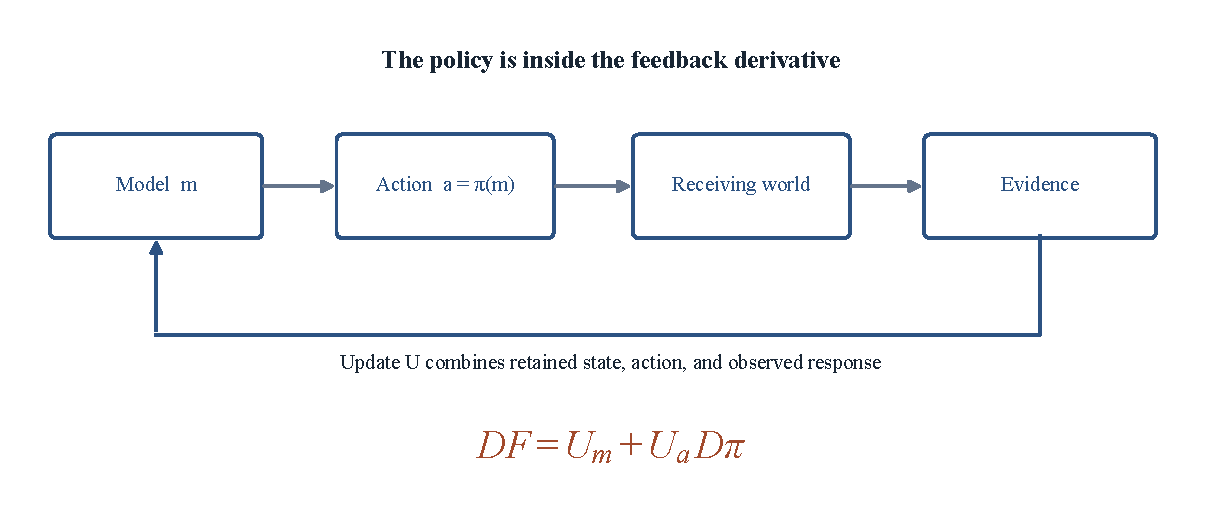
\includegraphics[width=\textwidth]{assets/model-action-loop.pdf}
\caption{The model changes the action, which changes the evidence used in the next update. $U$ combines retained state, action, and environmental response. The derivative of the composite map contains both the direct term and the path through the policy.}
\label{fig:mechanism-model-action-loop}
\end{figure}
\subsection{Compression That Supports Intervention}

Call a representation \emph{intervention-ready compression} when it preserves enough structure to guide a specified class of actions within stated error and risk tolerances. The phrase names a practical requirement. Causal inference already supplies rigorous distinctions among observation, intervention, and counterfactual reasoning \cite{pearl2009causality}.

Records can contain evidence about all three. Text is not confined to surface correlation: it can describe experiments, mechanisms, and failed interventions. A learner can recover causal structure from such records when the data and assumptions permit it. Nevertheless, accurate prediction of records alone does not certify a particular intervention model.

The transition to action asks a different question. If the system changes this variable, with these constraints and this history, how does the distribution of later states change? A drug may alter the probability of an outcome without determining every patient's response. A control signal may shift a trajectory distribution without producing identical motion on every attempt. Actionable causality does not require determinism.

Which variables must be retained? A local sensitivity screen offers one limited answer:
\begin{equation}
 \left|\frac{\partial f}{\partial x_i}\right|\sigma_i>\theta.
\end{equation}
For a scalar state-transition quantity $f$, the left side estimates the effect of uncertainty $\sigma_i$ in variable $x_i$. The threshold $\theta$ must use the same units as that effect. A variable whose estimated effect exceeds the task's tolerance deserves attention.

This is a first-order approximation. Interactions, correlated uncertainties, discontinuities, and rare severe events can defeat it. A variable can have a small local derivative and still determine whether a system crosses a catastrophic boundary. Selecting a model therefore requires more than ranking ordinary sensitivities.

Scale matters for the same reason. At one scale, friction can be represented by an effective coefficient. At another, surface texture, deformation, temperature, and contact history may have to reappear. The right representation is the one that remains useful under the interventions actually contemplated.

Simulation buys controlled variation. Real feedback tests transfer. Domain randomization, demonstrations, online learning, and model-based planning arrange this exchange differently \cite{tobin2017domain}. Their common bill includes observations of how the receiving world responds.

Those observations can be expensive and slow. In drug development, a historical estimate based on selected company data included both unsuccessful projects and the financing cost of time \cite{dimasi2016}. Such estimates are sensitive to sample and accounting choices; no single figure is the timeless price of discovering a drug. The robust point is that copying a report and obtaining a new clinical response draw on different resources.

The 2026 rentosertib program makes the distinction current. An AI-associated discovery and development process had reached a Phase III program, with the first patient announced in September \cite{insilico2026phase3}. Enrolling a trial creates a route to evidence. Its announced follow-up period is still time that has to pass. The label “AI-discovered” cannot supply the missing outcomes.

Resource barriers determine how much a real observation costs. Temporal rigidity determines when it becomes available. Topological coupling determines where an intervention's effects travel. A world model operates inside these constraints, using a limited budget of responses to improve future decisions.

Reversibility changes the budget. A discarded software hypothesis can often be recovered from a log. An unnecessary physical collision may destroy the state needed to try again. In a clinical or ecological setting, some uncertainty cannot be resolved by unrestricted experimentation. The model must then support conservative margins, staged interventions, and explicit decisions about which uncertainty remains.

Other agents complicate the target further. Once a model is deployed, people can adapt to it, exploit its categories, or withhold the evidence it expects. The representation that worked before deployment may become inadequate because deployment succeeded in changing behavior. Monitoring must therefore ask whether the transition rule itself is drifting.

Failure reveals an omission, but not every failure identifies it uniquely. A missed grasp can reflect perception, calibration, mechanics, or planning. A weak treatment response can have several explanations. Learning requires experiments and diagnostics that distinguish among them. More failed actions without better attribution can consume the feedback budget without improving the model.

The ambition is demanding and concrete: use finite, costly, noisy responses to build a representation that continues to support action after action has changed the world. A model needs to retain what the next consequential intervention will make matter.

That requirement leads directly to the body. Some of the variables a model could track are handled instead by elasticity, geometry, reflex, and metabolism. The next chapter examines this older form of compression, built into matter and paid for through evolution, development, and maintenance.

\chapter{Life, Bodies, and Movement}

A road responds through friction, inertia, and traffic. An organism also responds through metabolism, repair, immunity, adaptation, and memory. Its response can change the pathway through which the next intervention must enter. The receiving medium helps determine what intelligence has to become.

\section{Genes Are Physical Structures}

\subsection{What the Code Metaphor Leaves Out}

DNA can be copied, edited, and transmitted. A change in sequence can alter the production of a protein. The analogy with code captures something substantial: a relatively stable sequence participates in a reproducible process with consequences beyond itself.

The analogy becomes misleading when it suggests a clean separation between a program and interchangeable hardware. A sequence acts through cellular machinery, regulation, molecular interactions, development, and environmental conditions. It has no biological function in isolation from a system capable of using it.

Software depends on an execution environment too. The difference is practical rather than metaphysical. Engineers can often specify and stabilize a software platform, inspect its interfaces, and replace a component while preserving a contract. In a cell, the execution environment is itself a living product of the network being changed.

The path from genotype to phenotype passes through chromatin state, transcription, RNA processing, translation, folding, molecular interaction, metabolism, and tissue organization. Some variants have large and comparatively direct effects. Many traits involve numerous variants and environmental influences \cite{manolio2009finding}. Neither pattern makes a nucleotide change an abstract text edit.

Binding gives a small quantitative example. Define the mutation-induced change in standard binding free energy as mutant minus wild type. For dissociation constants measured under comparable conditions,
\begin{equation}
 \Delta\Delta G_{\mathrm{bind}}
 =RT\ln\frac{K_{\mathrm d}^{\mathrm{mut}}}
                 {K_{\mathrm d}^{\mathrm{wt}}}.
\end{equation}
The ratio is dimensionless. If the mutant has a dissociation constant ten times larger, binding is weaker and the free-energy change is positive: about $5.7\,\mathrm{kJ\,mol^{-1}}$ near room temperature. Reversing the energy convention reverses the sign, so the convention must accompany the equation.

The logarithm connects a modest energy difference with a large change in equilibrium affinity. The biological effect still depends on concentration, kinetics, localization, competing partners, and the network in which binding occurs. A binding measurement is one layer of an intervention's meaning.

This is a useful way to read biological information: a sequence changes possible material processes. Its “semantics” is realized in rates, flows, structures, and survival under particular conditions.

\subsection{An Execution Environment with a History}

An organism's machinery was not assembled from a clean specification. Existing structures were modified, duplicated, repurposed, and retained under changing selection pressures. Drift and historical contingency also contributed. Evolution produces viable descendants, rather than a guarantee of engineering optimality.

What appears redundant in one assay may matter under another condition. A backup pathway can become essential under stress. A regulatory element can matter only at one developmental stage. Conversely, a conserved or persistent structure should not automatically be assigned a hidden adaptive purpose. Its role has to be investigated.

The important point is dependency. Later structures can become reliant on an earlier arrangement. Replacing that arrangement then requires more than improving its isolated performance. The same problem appeared in technological networks; biology implements it in molecules, cells, tissues, and development at once.

The manuscript calls this deep embedding \emph{hyper-embodiment}: biological information is constituted within a body--environment history, rather than installed in a body after being designed elsewhere. The term emphasizes the depth of coupling. It does not establish that every sequence encodes environmental history or that adaptation is the only source of biological structure.

An eye works in a world containing light, optical media, moving bodies, and objects worth detecting. A lung works within constraints imposed by diffusion, circulation, metabolism, and atmospheric composition. The relevant knowledge is partly in the arrangement of matter. There is no separate list of every environmental fact the arrangement exploits.

\subsection{A Target Is a Route Through a Body}

Biological coupling does not make intervention impossible. It makes pathways decisive. Receptors, enzymes, ion channels, transcription factors, immune checkpoints, and hormone systems can provide leverage over a larger state.

An effective intervention need not describe every component. It needs a sufficiently important, reachable, and tolerable point of influence. The route includes delivery, distribution, timing, persistence, clearance, and the system's response to being changed.

Different technologies encounter different routes. A small molecule must reach suitable concentrations at its site of action. An antibody must encounter an accessible epitope. An editing system must reach the relevant cells and act there. A cell therapy must retain the behavior on which its benefit depends.

Delivery is a physical problem. The limited packaging capacity of conventional adeno-associated viral vectors, for example, constrains what can be carried in a single vector \cite{naso2017adeno}. Tissue distribution and immune responses depend on the vector, payload, route, and patient. There is no universal “send to the body” interface.

Four layers help organize the difficulty:
\begin{enumerate}
 \item \textbf{Molecular realization:} a sequence change must become a physical change in expression, structure, interaction, or reaction.
 \item \textbf{Network coupling:} the local change propagates through interacting processes.
 \item \textbf{Historical dependency:} the network's current arrangement contains inherited constraints.
 \item \textbf{Access:} an intervention must reach the right place with a usable timing and safety margin.
\end{enumerate}

These layers explain why editing accuracy is a major achievement without being the entire achievement. “The intended sequence changed” and “the patient obtained a durable benefit” describe different endpoints.

The force of gene technology comes precisely from reaching deep into this machinery. Its success will be measured by the states it can reliably produce, through pathways a living system can tolerate.

\section{When a Living System Pushes Back}

An intervention changes an organism and can also change how the organism responds to further intervention. Receptors are regulated. Metabolic pathways compensate. Immune systems retain memory. Tissues remodel. A control surface that worked yesterday may have different properties tomorrow.

\subsection{The Meaning of Biological Thickening}

This gives biological resistance a nonlinear shape. A larger or faster input can bring diminishing benefit, greater toxicity, compensatory responses, or an entirely different outcome. In other settings a stronger, well-timed intervention is essential. The response has to be measured; dose, frequency, and speed are distinct variables.

Rheology offers a useful visual analogy. Some dense suspensions become more resistant to flow when sheared sufficiently strongly. Over a limited thickening range, a simple model is
\begin{equation}
 \eta(\dot\gamma)=\eta_b+k\dot\gamma^{\,n},
 \qquad k>0,\quad n>0.
\end{equation}
Here $\eta$ is dynamic viscosity in $\mathrm{Pa\,s}$ and $\dot\gamma$ is shear rate in $\mathrm{s^{-1}}$. Consequently $k$ has units $\mathrm{Pa\,s^{n+1}}$. The two terms have equal magnitude at
\begin{equation}
 \dot\gamma_\times=\left(\frac{\eta_b}{k}\right)^{1/n}.
\end{equation}
This is a crossover defined by the model, not a general prediction of a suspension's onset threshold. The expression describes neither all low-rate behavior nor discontinuous jamming.

For biology, the analogy identifies a question: does resistance to a specified intervention rise with its rate or intensity, and through which feedback? A pharmacological response is not measured in pascal-seconds. A positive rheological exponent cannot be assigned to an organism without defining a biological input, output, and empirical relation.

The useful content is mechanistic. Suppressing one pathway may recruit another. Increasing a dose may increase adverse effects faster than benefit. Compressing a treatment schedule may allow less recovery. These are testable responses; “life thickens” is the image that brings them into the same discussion.

\subsection{Control Surfaces That Move}

A drug enters a system of absorption, distribution, metabolism, elimination, tissue barriers, and changing receptor states. Its target is a route through this system. The route can vary with disease stage, age, genetic background, other treatments, and previous exposure.

The immune system makes the importance of regulation particularly clear. Both inadequate and excessive responses can be harmful. Cytokine storm describes a family of severe inflammatory syndromes with different triggers and mechanisms \cite{fajgenbaum2020cytokinestorm}. A useful intervention must fit the relevant mechanism and clinical state; generic enthusiasm for “boosting” or “suppressing” immunity is no substitute.

Genome editing adds another layer. An edit's downstream effect depends on the cells reached, the change made, expression, selection, and the affected network. A transient editing reagent can produce a persistent sequence change. Temporary exposure therefore does not imply temporary consequences.

By July 2026 the US FDA had expanded Casgevy's indication to eligible patients aged two and older with specified forms of sickle cell disease or transfusion-dependent beta-thalassemia \cite{fda2026casgevy}. The achievement is substantial. Its execution still involves a regulated cell-therapy process, rather than a downloaded repair.

The associated regulatory record also retains long-term safety follow-up requirements \cite{fda2026casgevyletter}. Approval and continued observation belong to the same system. A successful intervention does not make every later uncertainty disappear.

\subsection{The Price of Keeping a Body Online}

A living organism performs maintenance while continuing to function. Cells repair damage, regulate proteins, clear waste, and preserve boundaries. An intervention must fit around this ongoing work. Surgery, anesthesia, extracorporeal support, and transplantation can temporarily reorganize parts of the system, but there is no general shutdown button followed by a clean restart of the same organism.

This creates three recurring constraints. Some responses need time to appear. Some effects travel through coupled networks. Some resources are already committed to maintaining the current state. A treatment can improve one measurement while placing a new burden elsewhere.

Drug discovery illustrates the resulting pipeline. Better screening and design can improve which candidates enter testing. Later evidence still depends on exposure, follow-up, measurement, and comparison. The historical decline in research productivity called Eroom's law described an empirical pattern with several proposed explanations \cite{scannell2012diagnosing}. It was not a biological law forbidding improvement.

The current test is whether new methods improve useful output across the chain. Rentosertib's September 2026 entry into a Phase III patient-dosing stage supplies an observable milestone \cite{insilico2026phase3}. The outcomes of that stage remain to be established. Discovery speed and confirmation time can move differently.

Little's law clarifies the inventory without dictating the outcome:
\begin{equation}
 L=\lambda W.
\end{equation}
For a consistently defined, stable process, $L$ is average work in progress, $\lambda$ is average throughput through its boundary, and $W$ is mean time inside. All exits, including withdrawals and early failures, must be handled consistently. The relation does not require every item to succeed.

If throughput doubles while mean time stays fixed, average work in progress doubles. If arrivals exceed sustainable service capacity, a growing queue may have no stationary average to which the relation can be applied in that simple form. The equation by itself cannot show that more candidates leave approvals unchanged. Capacity, selection, success rates, and waiting times determine that result.

\subsection{Robustness, Aging, and Rhythm}

Robustness is valuable because it resists perturbation. That resistance can also make a desired change difficult. A pathological state may persist through mechanisms that stabilize the system locally. Treatment then involves shifting the dynamics, rather than merely deleting an isolated error.

Yet disease cannot be reduced to a body stubbornly defending itself. Infection, injury, inherited defects, malignancy, and degeneration involve different mechanisms. The network perspective is useful when it adds an explanation, rather than replacing diagnosis with a metaphor.

Aging exposes the limits of maintenance over time. Damage, altered regulation, cellular changes, and tissue interactions contribute in ways that research continues to disentangle \cite{lopezotin2013hallmarks}. Reproduction allows lineages to continue despite individual mortality. Neither fact proves that a particular lifespan is an unavoidable thermodynamic maximum.

The practical lesson is rhythm. Some interventions need urgency; some need recovery intervals; some require follow-up long after the initiating event. A mature biological technology identifies which clock governs which consequence.

Pushing harder may help, may saturate, or may recruit a new obstacle. The deep question is what the system does with the push.

\section{The Body Absorbs What the Model Leaves Out}

A robot plans a grasp. The object is heavier than expected, the surface is damp, and a cable is caught underneath. None of these surprises needs to be large. Together they can turn a plausible plan into a broken object.

Physical intelligence is the ability to keep acting through such departures. A body is one of its mechanisms.

\subsection{Residuals and Their Receiving Structures}

Use \emph{residual} here for a deviation not yet absorbed by the current model, sensing, mechanics, controller, or operating process. The term gathers several different quantities; it does not make them one measurable scalar.

A model omits a relevant variable. A sensor drifts. A contact slips. An actuator responds late. A remote operator sees an obsolete image. Some deviations are corrected locally. Others change the initial condition for the next action.

The distinction matters over a task chain. A short demonstration can begin with known objects in a prepared arrangement. A shift in a distribution center must handle repeated actions, wear, exceptions, and recovery. A household task adds uncertain ownership, fragility, privacy, and context.

Human hands combine soft contact, proprioception, muscle elasticity, reflex, and learned anticipation. Many adjustments occur without deliberate calculation. The body turns part of the control problem into a material response.

Passive dynamic walking made this principle visible in machines: appropriately arranged mechanics can organize motion using environmental energy, with much less active control than a rigid position-by-position description suggests \cite{mcgeer1990,collins2005}. Biological locomotion likewise exploits mechanics rather than commanding every degree of freedom independently \cite{full1999}.

Three layers are useful. Materials absorb shocks and adapt contacts. Sensorimotor loops correct deviations at short latency. Experience identifies which details require immediate attention and which can be ignored. The layers overlap continuously in action.

The ecological and embodied traditions place this coupling at the center of intelligence \cite{gibson1979,varela1991,gibsonpick2000}. Morphological computation asks how shape, compliance, and dynamics participate in control \cite{pfeifer2007,pfeiferbongard2006,hauser2011}. Moravec's observation about the surprising difficulty of ordinary sensorimotor skills belongs to the same history \cite{moravec1988}.

The body lets a model remain incomplete. That is a functional achievement, not an exemption from computation or physics.

\subsection{When the Hidden Work Becomes an Engineering System}

Machines can use the same design principle. A compliant gripper can simplify grasping. A fixture can remove ambiguity. A mechanical stop can prevent a dangerous configuration before software detects it. A robot need not imitate a human hand to perform a useful task.

What biology combines locally may nevertheless appear in a machine as separately designed subsystems: tactile sensing, slip estimation, timestamp alignment, force control, calibration, limits, diagnostics, and incident logs. Their interfaces become part of the operating burden.

Call the recurring burden \emph{interface debt}. Calibration must remain valid. Sensor data must refer to compatible times and coordinate frames. A replacement part must preserve a contract. A failure must be attributable to a place where someone can act.

For $n$ modules, the number of possible pairwise relationships is
\begin{equation}
 N_{\mathrm{possible}}=\frac{n(n-1)}{2}.
\end{equation}
A good architecture does not implement all of them. Hierarchy, shared standards, and sparse interfaces can reduce the actual burden dramatically. The expression warns against uncontrolled interdependence, rather than predicting a quadratic cost for every robot.

Residuals can propagate through these relationships. A small timing error corrupts state estimation; an incorrect estimate changes the commanded force; the force changes the object; the changed object produces the next observation. The system needs a sufficiently coherent account of the present to remain inside a recoverable region.

Some engineering makes the work explicit because explicitness is valuable. Logs, modular boundaries, and diagnostics can improve repair and audit. Biological integration is not uniformly superior: it can conceal faults and make replacement difficult. The relevant comparison is the cost and reliability of the complete arrangement.

\subsection{Prediction and Recovery}

A better model can reduce errors, avoid dangerous contacts, and exploit existing hardware more effectively. It can eliminate particular failure modes. There is no conservation law requiring each removed error to reappear elsewhere.

The physical limits remain specific. A model cannot make an actuator deliver force it does not have, restore a broken part by revising a sentence, or observe a hidden variable without a source of information. The design task is to identify which deviations can be predicted away, which need local correction, and which require interruption or outside help.

Long task chains make this visible. Imagine clearing a kitchen counter. A cup may contain water. A medicine package may belong in a particular place. A charging cable may entangle another object. Grasping changes the scene; placing an object changes access to what remains. Success depends on detecting when a previous assumption has ceased to hold.

Failure can become abrupt near a capability boundary. A slip remains recoverable until a force, geometry, or reaction-time limit is crossed. Beyond it, the object falls. The average accuracy of preceding perceptions may say little about that threshold.

Abrupt failure is a hypothesis to investigate in a given task family, not an inevitable property of robots. Recovery policies, better mechanics, and safer environments can produce graceful degradation. Useful measurements include task length, disturbance magnitude, intervention rate, recovery time, and maintenance cost.

A system that sustains longer tasks with slowly rising support requirements has achieved something stronger than a collection of isolated demonstrations. It has expanded the region in which residuals remain manageable.

\subsection{What Evolution Has Already Amortized}

Human action looks light partly because its preparation is absent from the immediate scene. Evolution shaped materials and reflexes over many generations. Development calibrated a particular body. Practice refined particular skills. The built environment then adapted doors, handles, stairs, tools, and signs to people.

This is \emph{evolutionary amortization}: the costs of obtaining a capability were distributed across a history that is not charged to the next use. It is an accounting perspective, not a claim that evolution optimized a financial objective.

If a consistently measured formation cost $C$ is allocated across $N$ uses, the average allocated cost is
\begin{equation}
 \bar c=\frac{C}{N}.
\end{equation}
The relation is bookkeeping. It supplies no measured value for the cost of evolution, and energy, years, injuries, and lives cannot simply be added as interchangeable units. Development and cultural preparation also recur; they are not a single sunk bill for the whole species.

Machines have their own amortization. Training, design, tooling, and a validated procedure can be reused across units. They also offer advantages biology does not: high loads, exact repetition, replaceable parts, and operation in hostile environments. The comparison changes with the task.

Open-world manipulation happens to demand a combination of compliance, sensing, repair, and flexible context handling for which biological bodies have a long history of adaptation. Reproducing the useful combination can require work in mechanics, data, models, and operations at once.

The GXO and Agility expansion announced in October 2026 is a revealing kind of progress: extend a specific logistics role from an operating site to additional sites \cite{gxo2026digit}. The bounded task and receiving workflow help define the next engineering step. Announced expansion and sustained performance at the new sites remain different evidence.

Physical AI matures by constructing a dependable ecology of body, model, controller, environment, and support. The object of design is the entire recoverable loop. An impressive brain is one component of that ecology; the body determines which mistakes the loop can survive.

\section{Exploration, Control, and Verification}

“More intelligent” hides several different ambitions. A system might produce more ideas, act with less delay, consume fewer resources, or offer stronger assurance. Progress can improve several at once. Designing an actual system still requires deciding how much of each the task demands.

\subsection{A Constraint Triangle}

Resources include computation, storage, sensing, communication, actuation, redundancy, and maintenance. Time includes decision latency, observation windows, physical response, and recovery. Assurance includes the evidence and safeguards needed to trust a result in its intended use.

These demands create a constraint triangle. Faster action may use less evidence. Stronger assurance may require more testing, narrower scope, or additional hardware. A low budget may require a simpler task. The triangle is a design framework; its frontier must be measured for a particular system.

Energy shows why efficiency and total demand need separate ledgers. Let $D$ be consistently defined work performed during a period and $e$ electricity per unit of that work. Then
\begin{equation}
 E=De,\qquad
 \frac{\dot E}{E}=\frac{\dot D}{D}+\frac{\dot e}{e}.
\end{equation}
The second identity assumes positive, differentiable quantities. The growth rates have units of inverse time. Better efficiency can coexist with rising total consumption when demand grows faster.

The IEA's 2026 work on AI and electricity documents precisely why these accounts need to be separated: task-level improvements can accompany rapid expansion of infrastructure demand \cite{iea2026questions,iea2026powering}. The task definition matters. A token, a completed service request, and a solved engineering problem are different units of useful work.

Assurance has an equally concrete boundary. As of September 2026, the FDA reported more than 1,600 AI-enabled medical devices authorized for marketing in the United States \cite{fda2026aidevices}. Each authorization concerns a particular device and intended use. The regulator's public list is also a periodically updated identification resource with stated coverage limits \cite{fda2026ailist}. Counting entries measures a deployment record; it does not measure unrestricted medical competence.

Some checks can become much faster through better proofs, tools, or experimental design. Others depend on waiting for a physical event or obtaining enough exposure to estimate a risk. “Verification takes time” becomes useful only when the project identifies which part of the time is reducible.

At a fixed budget, one can write
\begin{equation}
 B_{\mathrm E}+B_{\mathrm C}+B_{\mathrm V}=B,
\end{equation}
where the three allocations support exploration, control, and verification in a common accounting unit. Shared infrastructure must be allocated consistently. The equality expresses a budget, while the shape of the tradeoff remains an engineering question.

\subsection{Three Jobs for Intelligence}

\textbf{Exploration expands the candidate space.} It generates designs, hypotheses, explanations, molecules, and strategies. Its value lies partly in reaching alternatives that established procedures would miss.

Exploration benefits from cheap rejection. A surprising proposal can be useful even when many neighboring proposals fail. A fabricated factual premise, however, is still an error when presented as evidence. A good exploratory interface marks the difference between a hypothesis worth investigating and a fact on which the investigation may rely.

\textbf{Control keeps action inside a usable region.} It responds to disturbances, manages limits, coordinates timing, and decides when to degrade or stop. In a power system, aircraft, production line, or vehicle fleet, novelty is useful only when the resulting behavior fits the safety and performance envelope.

Control purchases reliability through appropriate sensing, mechanics, feedback, redundancy, and operating constraints. The strongest controller may be the one that refuses an action early enough to preserve recovery.

\textbf{Verification exposes what the other two have missed.} It checks sources, searches for counterexamples, challenges assumptions, measures failure modes, and investigates delayed consequences. Its output can be a proof, an estimate, a failed test, or a narrower claim.

Verification has its own productivity. A better test can reject a weak design earlier. A reusable proof can remove repeated checking. An independent observation can resolve an expensive dispute. Slow feedback deserves investment in informative experiments, rather than ceremonial caution.

\begin{table}[ht]
\centering\small
\begin{tabularx}{\textwidth}{@{}lYYY@{}}
\toprule
& Exploration & Control & Verification\\
\midrule
Primary question & What might work? & What action keeps this usable? & What has actually been established?\\
Useful output & A promising candidate & A stable, bounded trajectory & Evidence about a claim and its limits\\
Failure to watch & Candidate volume mistaken for progress & A locally sensible correction that destabilizes the whole & A convincing check that misses the relevant failure\\
\bottomrule
\end{tabularx}
\caption{Three functions that can share models while requiring different evidence and interfaces.}
\end{table}

\subsection{The Architecture Between Them}

These functions may run in one model or in many. Functional differentiation does not dictate a particular number of agents. It dictates inspectable handoffs.

How does a candidate enter a test? What evidence permits execution? How does execution revise the next candidate? Who can interrupt the process? Which failure invalidates a previous approval? A system's answers to these questions determine how much general capability it can use safely.

A general model can coordinate search across domains while specialized loops handle contact, timing, or proof checking. The upper layer becomes more useful when the lower layers expose reliable contracts. The result may feel like a single intelligence to its user even though its assurance comes from several mechanisms.

The competition is consequently architectural as well as computational. Better models increase what can be proposed. Better interfaces increase what can become dependable action.

\section{Where People Remain in the Loop}

The useful place for a person cannot be read from a permanent list of uniquely human skills. Machines change. Tasks change. Institutions assign rights and responsibilities. Three questions make the comparison more durable: who performs the whole task efficiently, who improves the feedback structure, and who has standing to decide that a result is good enough?

\subsection{The Whole Energy Bill}

The adult brain operates at a power level on the order of tens of watts, while the whole body has a larger, activity-dependent metabolic demand \cite{smil2015power}. Comparing that brain figure with the peak power of a data center mixes boundaries.

For system $s$, a useful decomposition is
\begin{equation}
 E_s=E_{s,\mathrm{sensing+computation}}
     +E_{s,\mathrm{execution}}
     +E_{s,\mathrm{support}},
 \quad s\in\{\mathrm{human},\mathrm{machine}\}.
\end{equation}
All terms use the same energy unit, task, quality standard, and completion window. Categories must be mutually exclusive. Where biological functions cannot be separated cleanly, a total measured at the chosen boundary is better than a fictional allocation.

A maintenance worker in an unfamiliar building handles stairs, labels, obstructed access, tools, conversation, and an incomplete description of the fault. A machine serving the same role may need remote support, sensing redundancy, and recovery equipment. The person's training, fatigue, injuries, transport, and organizational support also belong in the chosen comparison.

Body mechanics can reduce the need for active correction on both sides. So can environment design. Standardized racks and containers change the task, often enough to make automation attractive. An open environment and a human-shaped environment are not identical categories: many supposedly natural tasks already benefit from years of design around people.

Task-matched measurement determines the energy result. Reliability, cost, dignity, and service quality then determine how much that result should matter.

\subsection{Different Responses Can Stabilize a System}

Uniform automation can create common responses. Many participants read the same signal, use similar models, and act together. A local correction becomes a collective shock.

For linear channels responding at one frequency, the combined amplitude is
\begin{equation}
 G_{\mathrm{sum}}=
 \left|\sum_{i=1}^{N}g_i e^{\mathrm{i}\varphi_i}\right|.
\end{equation}
Here $g_i$ is an amplitude gain and $\varphi_i$ a phase in radians. Aligned phases add coherently; dispersed phases can partly cancel. This is an amplitude relation. Closed-loop stability requires the complete feedback structure.

Randomized backoff, staggered execution, independent review, and differing information sources can reduce harmful synchronization. People sometimes provide such differences. They can also share biases, follow the same incentives, or respond too late.

The goal is useful diversity of response. It can be supplied by people, software, institutions, or a combination. Its value has to appear in the system's behavior.

Human supervision has particular requirements. The operator needs relevant information, time to act, maintained skill, and real authority. Research on the ironies of automation and human use of automation explains why a nominal person in the loop can be a weak safeguard \cite{bainbridge1983ironies,parasuraman1997humans}. A person asked to rescue an opaque process after long inactivity may have less usable control than the diagram suggests.

\subsection{Meaning Enters the Stopping Rule}

A search can stop because it has reached a time budget, an error threshold, or a convergence test. A society also needs to decide when the result may be relied upon.

Let $\mathcal A$ be the set of states meeting a specified quality and risk requirement. A first arrival can be written
\begin{equation}
 t^\ast=\inf\{t\geq0:\mathbf{x}_t\in\mathcal A\},
 \qquad \inf\varnothing=+\infty.
\end{equation}
The expression defines a stopping event. A real program can also exhaust its budget and report failure. The important social content lies in choosing and revising $\mathcal A$.

Which errors are tolerable? Whose risk counts? What evidence permits deployment? Who can contest the decision? These questions bring meaning into the admission conditions for action. They can be informed by models, yet their authority comes from the people and institutions entitled to set them.

Metrics become part of behavior when attached to rewards and penalties. Goodhart's and Campbell's observations describe why a successful measurement can become a target that distorts the activity being measured \cite{goodhart1975problems,campbell1979assessing}. Admission conditions need review and appeal as well as automatic checking.

Expertise and standing are different. A specialist may best estimate a failure probability. The people exposed to that failure still have interests and rights in deciding whether the exposure is acceptable. A workable system connects the two through intelligible evidence, accountable decisions, and remedies.

The human position is therefore specific. Energy claims need fair measurement. Stabilizing roles need a demonstrated feedback benefit. Decision rights need legitimate authorization. As technology changes, these criteria can guide a changing division of work without turning every capability update into a referendum on human worth.

\section{Cars Improve Faster than Transport Systems}

Replace an engine and the street stays where it was. The bridge, parking structure, school catchment, suburban subdivision, and morning schedule remain. Transport is a useful specimen of technological viscosity because its hardware is entangled with the organization of everyday life.

\subsection{A Powertrain Is One Layer}

Electric motors offer high efficiency, rapid control, and a different maintenance profile from combustion engines. Batteries move costs into materials, manufacturing, charging, thermal management, and eventual reuse or recycling. A proper comparison follows both systems through their lifecycles.

The IEA's 2026 assessment finds lifecycle emissions savings for battery electric cars under its stated comparisons, despite higher manufacturing emissions associated with batteries \cite{iea2026evlifecycle}. The size of the saving depends on vehicle, electricity, use, and lifetime. Counting the battery bill does not justify erasing the operational benefit.

The distinction that matters here is between improving a vehicle and reorganizing movement. An electric car still occupies road and parking space. A heavy battery does not invalidate electrification; a better powertrain does not settle congestion, access, or land use.

Transition costs also need a long boundary. Charging infrastructure is an added investment; fuel extraction, refining, distribution, and combustion vehicles already have investment and operating bills. Minimizing immediate change can preserve a more expensive long-run system. Engineering can compare alternative transition paths using lifecycle cost, emissions, service quality, and risk. Mechanical least action supplies no automatic verdict.

The strongest critique of automotive spectacle is therefore a precise one: the sales chart for a new powertrain cannot stand in for the performance of the transport system.

\subsection{Optimize Access, Then Movement}

People need access to work, education, care, other people, and goods. Movement supplies some of that access. Urban design, service location, remote work, and reliable local provision can reduce how much movement is necessary.

The road-flow identity is
\begin{equation}
 q=\rho v,
\end{equation}
where $q$ is vehicles per unit time, $\rho$ is vehicles per unit distance, and $v$ is space-mean speed over a consistent segment. Increasing speed need not increase throughput because safe spacing, density, and traffic dynamics change with speed.

Vehicle technology can affect these relationships: automation may change headways, vehicle sizes may change space use, and new operating patterns may change demand. The identity itself determines none of those behavioral responses.

Private cars offer flexible access, privacy, and storage. In low-density places or for complicated care and work schedules, those benefits can be decisive. The same arrangement commits households to purchasing, parking, maintaining, insuring, and often driving a rarely fully utilized asset.

Once housing, commerce, schools, and roads develop around car ownership, individual choices reinforce the structure. A household may rationally buy a car because the system has made alternatives poor. Treating the purchase as an isolated preference misses the dependency.

“Effective movement” means movement that delivers the intended access or goods. Empty repositioning, avoidable detours, searching for parking, and trips created by poor coordination consume the network without supplying the same benefit. An efficient transport policy has to see them.

\subsection{Ownership Versus Operations}

Electrification changes propulsion. Fleet operation changes how vehicles are used. These are separate axes.

A shared fleet can spread vehicle costs over more trips, centralize maintenance, and reduce some parking needs. It also incurs dispatch, cleaning, support, repositioning, and platform costs. Empty miles and demand induced by cheaper travel can increase traffic even when the fleet uses fewer vehicles than an ownership-based alternative.

Autonomous operation changes the labor bill and operating possibilities. It adds a requirement to establish reliable behavior within an operating domain, manage exceptions, maintain sensors and software, and allocate responsibility. In mixed traffic, the vehicle acts inside a social environment designed largely around human interpretation.

Waymo's October 2026 announcements illustrate the levels that need separating: expanding service in existing markets is a different activity from preparing and validating a new city \cite{waymo2026expansion,waymo2026madrid,waymo2026toronto}. Neither an impressive drive nor an announced future market alone establishes a complete service.

High utilization can reduce embodied cost per passenger trip while increasing wear, maintenance intensity, and reliance on the operator's systems. Concentration may simplify some household interfaces while creating larger dependencies on a few service providers. The three viscosity coordinates can move in different directions.

\subsection{Could the Private Car Become a Yacht?}

A provocative possibility follows. If dependable fleets provide most ordinary journeys at attractive cost, private ownership could become less necessary and more elective. Some cars would remain prized for pleasure, control, identity, collecting, or unusual journeys. In those markets, ownership would resemble a yacht more than a utility connection.

The yacht analogy describes a conditional structural shift. Its conditions are demanding: coverage, waiting time, price, accessibility, child transport, luggage, rural service, privacy, resilience, and trust. A fleet that fails them leaves substantial reasons to own a car.

This is a better proposition to test than declaring that ownership will disappear. Watch whether households with adequate service actually give up vehicles, which trips remain expensive to serve, and how the network's total vehicle-kilometers change.

Dense corridors still favor high-capacity transit. Short trips often favor walking and cycling. Freight has different loads, schedules, and terminals. Low-density trips need flexible service. No one vehicle can take over all these tasks at the same physical cost.

Resilience also needs alternatives. A software failure, severe weather event, power shortage, or operator collapse can expose the weakness of a highly concentrated service. Spare capacity and independent routes have a bill; their value appears when a preferred route fails.

The future of transport can be sharper than the future of the car. The decisive measure is reliable access per unit of whole-system cost, including space, time, energy, harm, and resilience. Some improvements arrive inside a vehicle. Others arrive when the system needs fewer vehicles to do the same useful work.

\section{The Third Dimension Has an Operating Bill}

A river can make a short straight-line distance into a long journey. A mountain, damaged bridge, or isolated island can make the road network the principal obstacle. Flight becomes valuable when avoiding that obstacle is worth the cost of leaving the ground.

\subsection{Less Road, More Airspace Coordination}

Low-altitude aviation exchanges continuous surface infrastructure for vehicles, terminals, energy, navigation, weather information, separation, maintenance, and responsibility. A route through air needs no pavement along every meter. It still needs an operating order.

The range of useful aircraft is broader than the electric air taxi. Helicopters, conventional light aircraft, small cargo drones, and electric vertical-takeoff designs serve different payloads and missions. Electrification, autonomy, and vertical takeoff are independent design choices, even when one product combines them.

The question is whether a mission is worth flying. Inspecting a transmission line, carrying a time-critical medical sample, reaching a cut-off settlement, and moving a commuter between two well-served districts offer different alternatives and different values of time.

At low traffic density, a demonstration can rely heavily on special arrangements. At higher density, identification, separation, lost-link procedures, landing alternatives, and compatible communications become shared infrastructure. The third dimension adds freedom of route and a new coordination problem.

\subsection{The Battery Has to Fly Too}

Weight is especially unforgiving in hover. Ideal actuator-disk momentum theory gives the induced power
\begin{equation}
 P_{\mathrm i}=\frac{(mg)^{3/2}}{\sqrt{2\rho A}},
\end{equation}
where $m$ is total mass, $g$ gravitational acceleration, $\rho$ air density, and $A$ effective disk area under the model's assumptions. For fixed $A$ and $\rho$, doubling mass multiplies this ideal induced power by $2^{3/2}$, about $2.83$.

Actual shaft and electrical power also include aerodynamic losses, profile power, drivetrain efficiency, and auxiliaries. Interacting rotors complicate the effective area. The ideal relation is a lower-bound model for a specified configuration.

Battery endurance needs a second piece of accounting. Let $m_0$ be fixed non-battery mass and $m_b$ battery mass, with usable specific energy $e_b$. Holding disk area and effective efficiency $\epsilon$ fixed gives
\begin{equation}
 t_{\mathrm h}\approx
 \frac{\epsilon e_b m_b\sqrt{2\rho A}}
      {g^{3/2}(m_0+m_b)^{3/2}}.
\end{equation}

At first, adding a battery increases endurance. Eventually its added energy loses to the rising power needed to carry the whole aircraft. In this deliberately simplified model, differentiating with respect to $m_b$ places the maximum at
\begin{equation}
 m_b=2m_0.
\end{equation}
That is a two-thirds battery fraction, not a practical design recommendation. Structure, power capability, reserve requirements, thermal limits, changing rotor size, and payload can move or preclude the optimum.

The often-quoted $t_{\mathrm h}\propto m^{-1/2}$ scaling assumes usable stored energy proportional to total mass, as with a fixed battery fraction across otherwise comparable configurations. “Add only battery” does not establish that proportionality for a fixed airframe. The distinction changes the shape of the engineering argument.

Cruise needs its own model. A winged aircraft can obtain lift differently from a hovering rotorcraft. Mission energy includes takeoff, transition, cruise, landing, reserves, and contingencies. A hover calculation alone cannot determine the range of an air taxi.

Liquid aviation fuel offers high specific chemical energy; batteries offer a different conversion chain, power response, and maintenance profile \cite{viswanathan2022challenges}. Comparing only fuel energy with cell energy misses propulsion efficiency and system mass. Comparing complete missions makes the tradeoff visible.

\subsection{A Flight Is One Step Toward a Service}

Certification separates several questions: is the design acceptable, was a particular aircraft built and maintained appropriately, and is the intended operation authorized? Flight capability is evidence within this process.

Joby announced the first flight of an FAA-conforming aircraft for its Type Inspection Authorization program in March 2026 \cite{joby2026conforming}. The announced milestone concerned a test aircraft and a certification path. It should be read at that level.

In September, Joby separately described an autonomous J208 tour using a converted Cessna Caravan and supervised operations \cite{joby2026j208}. This concerns a different aircraft and another part of the operating problem. Combining the two headlines into “an autonomous electric air taxi is certified for unrestricted service” would combine claims that neither announcement establishes.

The FAA's powered-lift framework and EASA's VTOL specifications show the institutional work needed alongside the aircraft \cite{faa2026aam,easa2026vtol}. Specific requirements vary by jurisdiction, aircraft, and operation. A certification obtained in one setting does not automatically authorize every other setting.

The social interface is broader still. Noise reaches people who bought no ticket. A forced landing needs a place to go. Weather can interrupt a route whose ground alternative is also difficult. Insurance and investigation need records that survive a failure.

\subsection{A Valuable Bypass Has a Defined Mission}

A useful comparison can be written in a common cost measure:
\begin{equation}
 C_{\mathrm{flight}}+C_{\mathrm{coordination}}
 <C_{\mathrm{ground\ alternative}}.
\end{equation}
The left side includes vehicle, energy, maintenance, reserves, terminals, communication, airspace services, and allocated risk. The right side includes the actual alternative, including detour, delay, and infrastructure where relevant. Avoid counting the same item twice.

Some requirements belong outside the scalar comparison. A service that violates an applicable safety or rights constraint does not become acceptable merely because a weighted cost happens to be low. Time-critical missions may also place a value on minutes that an ordinary commute does not.

The most compelling markets are those in which the ground route is unusually burdensome and a manageable air operation supplies a large benefit. This directs attention toward particular logistics, inspection, emergency, and geographic problems. Each can build evidence within a bounded operating domain.

Large forecasts for an aviation market cannot perform this mission-by-mission calculation. Nor does a spectacular prototype answer who will maintain the service on a wet Tuesday when equipment fails.

The durable value may accumulate in operations as much as in aircraft manufacturing: compatible navigation, weather services, maintenance, scheduling, insurance, terminals, and accountable oversight. Fragmented local platforms can recreate in the sky the interoperability problems flight was meant to bypass.

The third dimension is a route around some surface constraints. Its business exists where that route, with its whole operating bill, is better than the ground.

\begin{figure}[ht]
\centering
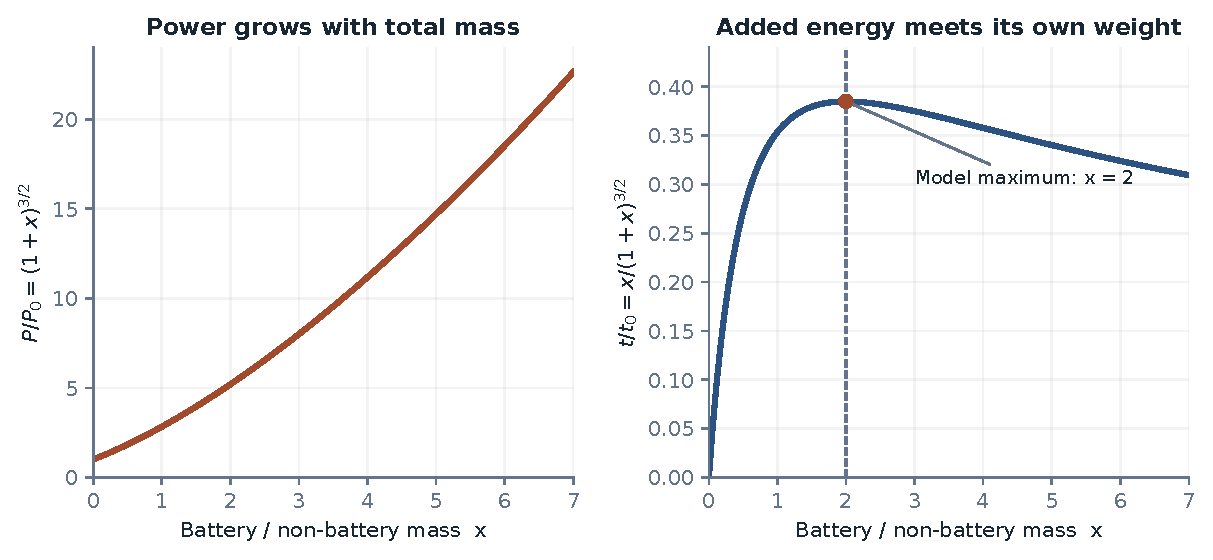
\includegraphics[width=\textwidth]{assets/hover-tradeoff.pdf}
\caption{Ideal hover at fixed disk area, air density, and efficiency. Here $x=m_b/m_0$, $P_0$ is the induced power for the non-battery mass, and $t_0=\epsilon e_bm_0/P_0$. The normalized endurance peaks at $x=2$. Structure, power limits, and mission profile add further constraints.}
\label{fig:mechanism-hover-tradeoff}
\end{figure}

\section{Manage the Regime, Not Just the Peak}

A factory, a hospital, and a transport network can improve a local optimum while making their interfaces harder to manage. The next question is how to keep systems with different response times working together.

\subsection{Several Clocks in One System}

Symbols can be copied quickly. A transformer can take a long time to procure. Clinical effects may take longer to characterize. The clocks belong to particular processes. A nerve impulse is fast. Training and validating a digital system can be slow.

For a specified process $i$, a useful ratio is
\begin{equation}
 De_i=\frac{\tau_i}{T_{\mathrm{drive}}},
\end{equation}
where $\tau_i$ is a characteristic relaxation time and $T_{\mathrm{drive}}$ the driving timescale in matching units. The Deborah number comes from material behavior. Applied to organizations or biological interventions, it is a timescale analogy whose variables need operational definitions.

When the receiving process relaxes much faster than its drive, successive changes may be absorbed separately. When the drive is fast relative to relaxation, unfinished responses can overlap and history becomes important. Neither a large nor a small ratio, by itself, proves instability.

A warehouse may change routing instructions every few seconds while staffing, training, and layout evolve over months. A grid can settle electrical disturbances rapidly while adding physical capacity takes years. A drug may engage a target quickly while long-term consequences remain unknown.

\begin{table}[ht]
\centering\small
\begin{tabularx}{\textwidth}{@{}lYYY@{}}
\toprule
Layer in a project & A relatively fast process & A slower receiving process & What can accumulate\\
\midrule
Digital & Generate a design & Integrate and verify it & Unreviewed changes\\
Industrial & Change an order & Build equipment or capacity & Backlog and commitments\\
Biological & Initiate an intervention & Observe adaptation and long-term effects & Unresolved exposure and risk\\
\bottomrule
\end{tabularx}
\caption{Timescale mismatches arise within each medium as well as between media. The project must identify the actual clocks.}
\end{table}

A single clock is often the wrong design. Fast loops can handle local disturbances, slower loops can change set points, and longer processes can review goals and capacity. Separation, buffering, and clear interfaces allow different rates to coexist.

\subsection{A Region in Which Recovery Remains Possible}

An operating system rarely needs to sit at one unchanging optimum. It needs to remain in a region where service continues, disturbances are absorbed, and recovery remains available.

The fluid image suggests three qualitative regimes: orderly throughput, amplified fluctuations, and loss of essential connection. In a real project these must be identified by measurements such as queue length, recovery time, failure correlation, reserves, and continuity of critical service. Hydrodynamic laminar flow and organizational stability do not share a universal threshold.

Local improvements can move a system toward a boundary. Shorter deadlines reduce recovery time. Lower inventories reduce buffering. More frequent policy changes reduce the period over which evidence can become interpretable. The same changes can also improve a poorly managed process. Their effect depends on the full loop.

Three design moves recur.

\textbf{Set a compatible pace.} Lengthen a decision cycle where the receiving process genuinely needs time. Elsewhere, accelerate measurement and correction so the process can tolerate a faster cycle. The aim is a fit between action and response.

\textbf{Decouple the rates.} Use buffers, reserves, staged rollout, modular boundaries, and local autonomy. A buffer's required capacity depends on the integrated excess inflow over the disturbance, rather than a rule that it must last longer than every slow process. A replenishable reserve and a one-time delay have different dynamics.

\textbf{Preserve checks that produce stability.} Verification, audit, maintenance, and accountable authorization consume resources while producing evidence, early fault detection, and recoverability. They are valuable when those functions work. Delays that supply no such benefit remain candidates for removal.

An optimization that includes reliability and recovery can choose these investments. The institutional problem appears when the benefits accrue beyond the person or department paying the immediate cost. The maintenance budget is local; the avoided collapse belongs to everyone.

Someone must hold the account across the slower cycle. Equipment life exceeds a management rotation. Ecological consequences can outlast a permit. Skill formation can outlast a product generation. Records and responsibilities need enough continuity to connect the benefit claimed today with the bill that arrives later.

The chapter's examples share an accounting discipline. A body absorbs contact uncertainty. An engineered system can reduce or relocate it. An electric vehicle changes energy flows. A fleet changes asset use. Flight changes the route and creates an airspace operation. In each case, progress is established by what the complete arrangement can now do for its total cost.

Costs can genuinely fall. A complete account establishes where and by how much. The danger is an incomplete boundary that counts an interface's speed while leaving its downstream consequences unrecorded.

That danger becomes acute when symbolic action becomes cheap. A plan, credential, image, or identity can be generated faster than anyone can determine what supports it. The next chapter examines what happens when the object, the evidence, and the accountable actor cease to line up.

\chapter{Existence and Collapse}

A generated city can be beautiful before it has a site. A proposed molecule can be elegant before it has been synthesized. A machine persona can be persuasive before anyone knows what obligations attach to it. Their immediate existence is easy to establish: there is an image, a structure, an interaction. Their claims on the rest of the world require a different account.

This chapter follows three separations. Existence differs from evidence. Evidence differs from authorization. The power to cause a consequence differs from the capacity and obligation to answer for it.

\section{What Exists, What Holds Up, and What May Act}

\subsection{The Weight of an Existence}

A rock, an organism, a corporation, and a generated character persist in different ways. A rock can remain stable without a continual supply of work. An organism maintains a far-from-equilibrium state through metabolism and repair. A corporation depends on records, assets, people, and legal recognition. A generated character can persist as data while depending on an operator for any continuing interaction.

The word “weight” has two uses here. Physical mass belongs to the material account. \emph{Consequential weight} concerns what it takes to establish, maintain, withdraw, and answer for something. A debt has little physical bulk as a database entry and substantial force in a person's life. Institutional recognition and enforcement connect the entry to that force \cite{searle1995construction}.

Consequential weight is best inspected as a profile:
\begin{equation}
 \mathbf w=
 (w_{\mathrm{establish}},w_{\mathrm{maintain}},
  w_{\mathrm{reverse}},w_{\mathrm{spillover}},
  w_{\mathrm{account}}).
\end{equation}
The components may use different units and need not be added. A weighted index is possible only after choosing a common scale and weights. A line of text and a bridge cannot be ranked by a universal number obtained from the word “weight.”

The profile nevertheless changes the questions one asks. What keeps the object available? What can undo its effects? Who pays for an error? Which effects outlive the carrier that initiated them?

Human representations have long created such connections. A map guides travel. A contract binds later conduct. A diagram precedes construction. Computation lets representations be transformed and tested before much of the physical commitment occurs.

Machine generation increases the volume and accessibility of these intermediate objects. The generated city exists as an image or plan. The proposed molecule exists as a specified candidate. The simulated robot action exists as a trajectory in a model. Each can be useful at that level.

The interesting question is which transition follows. A plan enters permitting and construction. A candidate enters synthesis and testing. A trajectory enters an actuator. A persona enters someone's decisions and relationships.

These are \emph{conversion edges}: routes by which a representation gains effects in another layer. Some go through heavy physical work. Others are light enough to traverse almost instantly. A fabricated message can change a person's judgment before anyone checks its origin. A generated command can reach equipment through an API. A score can alter a person's access to a job or loan.

The new asymmetry is the separation of cheap access from heavy consequence. A carrier may be easy to create and delete while its effects are difficult to recall. Erasing a false image does not erase every belief it helped produce. Reverting software does not reverse every transaction it authorized.

This is older than AI. Rumors, propaganda, fraud, and remote commands already exploited light carriers. Generation and automated execution change the scale, speed, variety, and number of pathways available. The receiving structures have to adapt to that change.

Representation can also become a source for further representation. Generated content enters public records, training sets, summaries, and subsequent decisions. Research on recursively trained models demonstrates degradation under particular synthetic-data arrangements \cite{shumailov2024ai}. The relevant issue is the information retained and refreshed across the loop, rather than whether any item has a synthetic origin.

An engineered sequence introduces another kind of edge if it is taken up by a biological process. Being writable, synthesizable, functional, heritable, and ecologically persistent are different properties. Each transition has its own constraints. The consequential weight appears where a process can continue beyond the designer's immediate control.

The map of existence therefore needs layers and edges. Layers describe what supports a thing. Edges describe what it can cause elsewhere. Accountability asks where the bill arrives after the edge has been crossed.

\subsection{After the Candidate Comes the Warrant}

A statement exists when it has been written. That fact supplies no evidence for its content.

Knowledge relevant to action needs a warrant: a reason the judgment can be relied upon for the use in question. A proof, calibrated measurement, replicated experiment, documented observation, and validated engineering model supply different kinds of warrant.

The distinction between representation and object is old \cite{ogden1923meaning}. Scientific practice makes it productive by building opportunities for claims to fail: tests, criticism, replication, prediction, and exposure to contrary evidence \cite{popper1934logik}. The method's strength lies partly in keeping a route open by which the world can reject an attractive account.

A warrant has two connected layers. One concerns how the claim was formed: source, instrument, data, method, and inference. The other concerns how it may be used: population, operating conditions, scale, uncertainty, and the consequences of error.

A laboratory result may be sound and still fail to support an advertised clinical use. A simulation may reproduce one condition and mislead outside it. A source can exist and be quoted accurately while being irrelevant to the decision at hand.

Machine systems can help build warrants. They can retrieve records, check calculations, produce proofs, propose discriminating experiments, and monitor outcomes. Their contribution should be evaluated at those interfaces. A generated answer does not have to remain a mere candidate if the system actually establishes the claim.

The pressure appears when candidate volume grows faster than confirmation capacity. For an illustrative queue,
\begin{equation}
 \dot Q=\lambda_{\mathrm{in}}
        -\lambda_{\mathrm{confirmed}}
        -\lambda_{\mathrm{rejected}}.
\end{equation}
All rates count candidates per unit time and use the same boundary. Confirmation and rejection both remove items from the unexamined stock. Some candidates can also be superseded or abandoned; a complete account includes those exits.

The backlog is not inevitable. Better filters, reusable evidence, and better candidates can increase effective capacity. The equation identifies where to look when a flood of plausible output fails to become a comparable increase in established results.

Fluency used to carry more information about the labor behind a statement. Producing a polished technical explanation often required training, sustained attention, and access to a professional setting. Models have made much of that surface cheaper. Readers therefore need signals attached to the warrant itself.

Traceable sources, executable calculations, identifiable assumptions, and independent checks can serve that role. Surface polish remains useful for communication. It has less power to certify the process that produced the claim.

The verification budget is finite. A society cannot investigate every generated suggestion at equal depth. Priority should depend on expected value, uncertainty, reversibility, exposure, and severity of plausible harm. Some claims need immediate checking; others can remain explicitly exploratory.

This is an allocation problem as well as an epistemological one. Who receives access to experiments? Which populations appear in a dataset? Which failures are counted? Which long-term effects receive a funded observer? The available warrants reflect those choices.

The most useful system makes its claims inspectable and revisable. It preserves the route from output to evidence and leaves a place where contrary evidence can enter.

\subsection{A Warrant Is Not a Permission}

A technically effective intervention can still be unauthorized. A correct prediction about a person does not grant the predictor unrestricted power over that person's opportunities. A feasible operation may impose costs on people who have no reason to accept them.

Knowledge answers what the evidence supports. Authorization answers who may do what, under which conditions, to whom.

The distinction becomes urgent with agents. A model connected to tools can move from describing a possibility to changing files, placing orders, sending information, or controlling equipment. Permissions and workflow determine the radius of effect.

Traditional accounts of action examine intention, reasons, and attribution \cite{anscombe1957intention,davidson1963actions}. An engineering account can begin earlier: regardless of how one interprets the machine's intention, a particular interface can trigger a particular state change.

Action commits a system to a path. Money is spent. A body is exposed. Equipment moves. An opportunity is granted or denied. Some parts can be reversed, while time, disclosure, trust, and other effects remain.

The residual uncertainty moves from the representation into the receiving system. A responsible authorization specifies how that uncertainty will be contained and who can answer for what follows.

Five functions make the connection concrete. Evidence identifies relevant failure modes. Limits contain the permitted action. Monitoring makes departures visible. Interruption and recovery restrict continuing harm. A responsibility structure connects remaining losses to identifiable obligations and resources.

These functions scale with the action. A private draft needs a different arrangement from an automated medical intervention. A reversible file edit and a public communication cross different boundaries even when the same model produces both.

Nominal human confirmation is weak when the person lacks information, time, competence, or authority. Meaningful control requires conditions under which a person can understand the relevant reasons, change the path, and interrupt it \cite{santoni2018meaningful}. Otherwise the confirmation button can turn an operator into an absorber of liability.

Authorization also changes over a system's life. A tool begins as optional advice, becomes the default, and eventually becomes infrastructure. A model update changes behavior. A new connector expands access. A workflow quietly removes the last review step. Each can enlarge the conversion edge without a single dramatic launch.

Continuous operation therefore needs continuing admission conditions. Scope, update policy, monitoring, incident handling, and revocation must remain attached to the deployed system. The authority to start is not an unlimited authority to continue under every future condition.

Existence supplies the object. Evidence supplies a warrant. Authorization supplies a legitimate route into action. Keeping these relations visible is the first defense against light carriers acquiring heavy consequences without a receiving structure prepared to bear them.

\section{Where the Consequences Return}

A robot can avoid a collision, detect damage, and request maintenance. A model can revise an answer after criticism. These are feedback capabilities. Accountability asks a further question: whose continuing position is changed by what happened?

\subsection{Body, Embodiment, and Answerability}

A body supplies a material boundary. Embodiment connects perception and action through that boundary. Answerability connects an action to continuing obligations, exposure, and response.

The distinctions matter because a machine's physical trace can be mistaken for a complete responsibility structure. A scratched casing is evidence of contact. A log is evidence that a record was made. Neither determines who compensates an injured person, investigates the incident, or carries the duty to prevent recurrence.

Self-repair can make the machine more capable \cite{terryn2017self}. It does not settle those questions. A tire bears friction; a deployer may bear the repair bill; a pedestrian may bear an injury. Several boundaries receive different consequences from one event.

The book uses \emph{consequence closure} for the degree to which action remains connected to a persistent, answerable boundary. This is a framework for practical agency and accountability. Conscious experience, moral standing, and legal personality require additional arguments; they cannot be measured by a repair log.

For a defined, finite, nonempty set of consequence items $C(a)$, one can illustrate return coverage by
\begin{equation}
 \kappa(B,a)=
 \frac{\left|\{c\in C(a):\rho_a(c)=B\}\right|}
      {|C(a)|}.
\end{equation}
$B$ is the boundary being inspected and $\rho_a$ assigns an item to its ultimate bearer in this simplified account. The result lies between zero and one.

The counting scheme matters. Dividing one injury into ten entries changes an unweighted ratio. Real consequences can be shared, uncertain, continuous, or incommensurable. A weighted or distributed assignment may be more useful in a particular investigation. The expression is an illustration of attribution, rather than a numerical test for personhood.

Complete return would also be a poor universal social goal. A driver cannot personally absorb every consequence of a collision; insurance pools some losses, emergency services provide support, and public rules distribute obligations. The aim is a justified and effective assignment, rather than forcing every effect back onto one individual.

For a living person, injury, memory, dependence, relations, and finite time connect action to an unusually persistent history. A replacement body is not an ordinary maintenance option. This gives human exposure a characteristic weight. It does not make people equally powerful, equally responsible, or equally able to escape a cost.

Machines can possess persistent identities and histories too, if an architecture maintains them. Replaceable components do not logically preclude continuity: corporations replace staff and hardware while retaining obligations. The practical issue is which boundary preserves the relevant identity and what binds it across replacement.

\subsection{The Corporation as an Engineered Boundary}

A corporation has no biological pain, yet it can own assets, undertake obligations, and face legal consequences. Law constructs a boundary through records, governance, representation, assets, and recognized continuity \cite{dewey1926historic}.

The analogy is powerful because it shows that answerability is partly an institutional achievement. Four features make the structure operational:
\begin{enumerate}
 \item An identifiable pool of resources and obligations.
 \item An identity that persists across relevant changes.
 \item Consequences that alter the boundary's future possibilities.
 \item A traceable arrangement of authority and duty.
\end{enumerate}

Actual corporate law varies, and actual corporations can externalize harm or leave victims uncompensated. Limited liability and insolvency can expose gaps. The structure supplies instruments for responsibility; its existence does not guarantee that the instruments distribute losses fairly.

An ordinary deployed model is usually a component inside such arrangements. Fining a provider affects the provider. Retraining changes the model's behavior. Withdrawing a service affects users and operators. Calling all of these “punishing the AI” conceals which boundary actually receives the consequence.

Versions need not destroy accountability. A record can preserve which version acted and a legal entity can retain obligations after changing its system. Conversely, keeping the same model name does not guarantee continuity if records and duties disappear.

The engineering and institutional jobs are complementary. Stable identifiers, versioned records, reproducible configurations, permissions, and operational logs make events investigable. Contracts, regulation, courts, insurance, and governance decide obligations and remedies.

\subsection{Distributed Action Needs Distributed Responsibility}

An output can pass through a foundation-model provider, adapter, application developer, platform, integrator, deploying organization, and end user. The contribution of each may depend on the others. A failure can arise from a combination no single component displays alone.

Many-hands problems predate AI \cite{nissenbaum1996accountability,floridi2013distributed}. Machine systems expand their speed and reach while making some causal contributions harder to inspect.

A schematic retention model writes
\begin{equation}
 R_n=R_0\prod_{i=1}^{n}\alpha_i,
 \qquad 0\leq\alpha_i\leq1,
\end{equation}
where $\alpha_i$ represents the share of a defined traceability measure retained at each handoff. It describes possible erosion when handoffs lose records or obligations. A well-designed handoff can preserve or improve the evidence, so attenuation must be established rather than assumed.

The policy question is where to attach duties. One approach identifies a party facing the affected user. Another follows control over the relevant risk. Another allocates duties across the chain and adjusts access to evidence. Their merits depend on the domain and legal setting.

Three separations are particularly dangerous: the party choosing the action differs from the party benefiting, the party holding the evidence differs from the party seeking redress, and the party assigned nominal responsibility lacks the power to change the process.

Accountability requires reconnecting these positions. A front-line employee should not become the default absorber for a system whose assumptions, update cycle, and permissions are controlled elsewhere.

The continuity that matters belongs wherever the duties can remain enforceable. It may sit with a provider, operator, professional, public body, or several of them. The model's output is the start of the inquiry, not its final answer.

This brings the problem back to people. As machines take over more production and institutions absorb more formal responsibility, the old connection between a person's skill, output, recognized position, and self-respect can loosen. The next three sections examine different ways that connection can fail.

\section{First Collapse: A Skill Loses Its Social Position}

A person can remain employed while the meaning of the job changes beneath them. The organization still wants a name on the workflow. It needs less of the craft through which that person learned to justify the name.

The first collapse is a loosening of the connection among capability, output, recognition, and position.

\subsection{The Interface Changes Before the Job Disappears}

A professional report once signaled more than a collection of sentences. It suggested access to information, trained judgment, command of a field, and time spent on the work. When a similar-looking report becomes cheap to produce, the signal changes.

The output may improve. The person's actual competence may remain. What weakens is the output's ability to distinguish the person who produced it.

A simple signal-detection expression makes the idea visible. For two Gaussian signal distributions with equal standard deviation $\sigma$,
\begin{equation}
 d'=\frac{\mu_1-\mu_0}{\sigma}.
\end{equation}
If the relevant distributions overlap more, discrimination becomes harder. This is an analogy for changing professional signals, not an estimate of AI's labor-market effect. A polished document now needs other evidence if it is meant to certify individual judgment.

Education has encountered related positional dynamics. Collins's account of credential competition examines how qualifications can become thresholds when their supply expands faster than the positions they distinguish \cite{collins1979credential}. The knowledge can remain useful while its exchange value changes.

Machine assistance can also complement a skill and raise its return. A capable accountant may serve more clients. An engineer may investigate designs previously beyond the budget. A novice may learn faster. The question is which complementary positions organizations actually create and who can reach them.

The familiar ATM case shows why task substitution and employment are different variables. Bessen's historical analysis describes how automation reduced teller work per branch while changes in branch networks and customer-facing work supported other demand \cite{bessen2015learning}. It supplies a mechanism, rather than a guarantee that each new automation wave will reproduce the same result.

Current evidence also needs this separation. The Stanford Digital Economy Lab's August 2026 revision, using payroll data through June, reports no widespread economy-wide displacement while documenting a substantial divergence for younger workers in exposed occupations \cite{brynjolfsson2026canaries}. The authors treat the findings as descriptive indicators, with reduced hiring an important channel. Aggregate stability can coexist with a difficult entry path.

That entry path matters beyond the immediate job count. Routine junior work can be part of how people acquire judgment. If automation removes the practice while retaining a demand for experienced reviewers, organizations need another way to produce the experience.

\subsection{Having the Result and Having Done the Work}

The second separation is personal. Receiving a finished result differs from participating in the process that made it possible.

Arendt distinguished labor, work, and action: recurring life-maintenance, durable making, and activity among plural people in a public world \cite{arendt1958human}. The distinction explains why a job can provide several kinds of attachment at once. It supplies income, an object produced, and a recognizable place among others.

Automating production can loosen those attachments together. Telling someone to “learn the tool” may solve the immediate delivery problem while leaving the question of recognition unanswered.

Kaczynski's account of a “power process” describes satisfaction through forming a goal, exerting effort, overcoming resistance, and achieving it \cite{kaczynski1995industrial}. The sequence is useful as a description of experienced agency. His larger claims about technological inevitability require their own arguments. The local mechanism does not establish a necessary political or historical endpoint.

In the book's coordinates, delegated work can make the user's immediate $R_p$, $T_p$, and $G_p$ small:
\begin{equation}
 \eta_p=\eta_0
 \exp(\alpha R_p+\beta T_p+\gamma G_p)
 \longrightarrow\eta_0
 \quad\text{as }(R_p,T_p,G_p)\to(0,0,0).
\end{equation}
The limit is the baseline $\eta_0$. More importantly, it concerns the user's experienced portion of a task. The provider and receiving world still have bills. This illustrative index does not quantify fulfillment.

The distinction is familiar outside AI. Paying for a meal and learning to cook both meet a need, but they produce different capabilities. Delegation can free time for something more meaningful. It can also remove an activity through which someone maintained confidence and competence. The resulting life depends on what fills the space.

Learned-helplessness research concerns controllability under specific experimental conditions \cite{seligman1967failure,maier2016learned}. It offers a useful question about whether action changes outcomes. It cannot be transferred wholesale into a diagnosis of people who use automated tools.

The stronger social question is whether people retain places where their judgments have intelligible effects. An environment that supplies endless results while rarely needing a person's sustained contribution can weaken that connection, even when its products are excellent.

\subsection{Demand Can Exist Without a Funded Position}

Care, education, repair, public service, and community life contain abundant unmet needs. Those needs do not automatically create paid roles. Budgets, procurement, professional rules, bargaining power, and institutions connect a useful activity to a livelihood.

Baumol's analysis explains how differing productivity growth can raise the relative cost of labor-intensive services \cite{baumol1967macro}. A society can become more productive overall while struggling to finance activities that still need time and presence.

This is why “people will move to more human work” is incomplete. The work needs an organization able and willing to pay, train, authorize, and retain the people doing it.

Arendt's analysis of superfluousness addresses a much heavier historical and political setting \cite{arendt1951origins}. The structural echo is the loss of an effective place in a shared world. It should sharpen attention to institutions, rather than turn ordinary workplace change into an automatic analogy with totalitarianism.

A person who loses an old occupational signal has not lost human worth. The economic interface has changed. Treating this solely as a motivation problem asks an individual to repair a relation that the surrounding system no longer offers on the old terms.

The first collapse can therefore occur without a layoff notice. People may still produce more, earn a salary, and use increasingly capable tools while becoming less certain where their judgment enters. A new position requires a real connection among contribution, learning, recognition, and authority.

When those connections remain weak, immediate feedback elsewhere becomes more attractive. That opens the second route of the chapter.

\section{Second Collapse: Feedback Stops Testing the Claim}

An image arrives before the user has learned to draw. A conversation offers attention without requiring another person's time. A game supplies a contest with carefully managed stakes. These experiences can be enjoyable, useful, and educational. Their effects depend on which feedback they preserve.

\subsection{A Feeling and the Process That Once Produced It}

Technical systems can separate a reward from some of the effort, uncertainty, or obligation that previously accompanied it. A finished artifact can arrive without practice in making it. An agreeable interaction can arrive without the negotiation of a reciprocal relationship.

The feeling is real. The question is what else develops with it.

A drawing tool can teach composition when the user compares, revises, and learns. It can also deliver an image while leaving those skills unchanged. A conversational system can support a person through a difficult moment. It can also occupy time that would otherwise sustain mutual obligations. The interface alone does not determine the result.

Fiction and play have always offered experience at a distance from its full consequences. Their value includes precisely that distance: one can explore a dangerous choice without living its worst outcome. Training simulators turn the same separation into a practical instrument.

The crucial connection is transfer. Which judgment is being trained, by which feedback, and against what independent standard? A simulator can alter a person's skills even though its aircraft is virtual. A system can produce intense feedback while teaching little about the world outside itself.

The second collapse occurs when the feedback ceases to test the claim for which it is being used. Enjoyment is used as evidence of competence. Reassurance is used as evidence of a relationship's reciprocity. A convincing explanation is used as evidence of a mechanism.

\subsection{Can Reality Interrupt the Representation?}

Baudrillard's account of simulacra follows changing relations between signs and what they purport to represent \cite{baudrillard1981simulacres}. Borges's map as large as the territory provides a related image of representation overwhelming its referent \cite{borges1946rigor}.

For this book, the operational test is straightforward: what can interrupt the representation?

An experiment can contradict an explanation. A load test can defeat a design. A source record can disprove a citation. A user can reject a proposed interpretation of their life. These are points at which the generating system does not control the answer.

Surface quality and external support can vary independently. A rough field note can preserve excellent evidence. A polished generated report can have none. There is no general law that signs become more convincing as their reality connection weakens; that combination is a dangerous possibility, not a mandatory sequence.

Goodhart and Campbell identify related problems when feedback becomes a target \cite{goodhart1975problems,campbell1979assessing}. A department learns to improve the reported measure. A researcher learns the benchmark. A platform learns which response receives a favorable rating. Each can increase the score while weakening its connection to the intended outcome.

The same issue appears inside machine learning. Training on evaluation items can inflate apparent generalization \cite{sainz2023nlp}. Recursively reusing model outputs can reduce information about less common patterns under particular conditions \cite{shumailov2024ai}. Carefully selected synthetic data can also be useful. The causal variables include quality, diversity, coverage, filtering, and access to fresh evidence.

Provenance tools supply one concrete response. C2PA's version 2.4 specification provides mechanisms for associating signed claims and content history with an asset \cite{c2pa2026spec}. Its validation concerns the provenance assertions and their integrity. It does not certify the truth of every depicted event or the honesty of a signer.

That distinction is an example of a healthy interface. A technical standard says which claim its check supports. Users then know which additional checks remain necessary.

The problem becomes severe when a representation environment insulates itself from contrary evidence. A ranking supplies the examples used to judge the ranking. A model supplies the explanation used to excuse its errors. An organization evaluates its performance using reports generated entirely inside the same reward structure.

An independent interruption point keeps such a system learnable. It can be a physical measurement, a fresh test, an external source, an appeal, or a person with authority to say that the representation has missed what matters.

\subsection{Who Arranges the Things We Want?}

Feedback changes desires as well as beliefs. Girard's triangular account places a mediator between subject and object: people often learn what to want by observing what others want \cite{girard1961mensonge}. Rivalry can intensify when model and observer compete in the same field \cite{girard1972violence}.

Digital platforms change the available mediators. A feed selects which lives, achievements, bodies, purchases, and opinions appear nearby. It can omit the preparation, financing, failure, and selection that produced the display. Viewers encounter a result without its cost structure.

Social-comparison research provides a narrower empirical framework \cite{festinger1954theory}. Studies of passive browsing and well-being investigate effects that differ by behavior, person, and setting \cite{verduyn2015passive}. More mediators do not automatically make everyone want the same thing. They can diversify aspirations, intensify local competition, or do both.

The pertinent design question is how selection changes the distribution of apparent possibilities. Which alternatives become visible? Which are rewarded? Which costs disappear from view? A person's choice occurs inside that presentation.

The temptation to treat material life as a dispensable inconvenience then has a long intellectual echo. Some ancient Gnostic traditions described a damaged material world and a route of escape through special knowledge. The analogy here concerns a preference for representation over the burden of living its counterpart. The historical traditions were diverse; a modern screen habit is not their direct continuation.

The stronger claim is practical. If a service supplies an attractive experience more cheaply than the activity it resembles, people have reason to shift time toward the service. Whether that shift enriches or narrows a life depends on learning, relationships, health, opportunity, and the alternatives actually available.

The test of authenticity is therefore not how painful an experience was, how many materials it consumed, or whether a computer participated. It is whether the claim made for the experience remains connected to something capable of correcting it.

When an experience is sold as competence, test transfer. When it is sold as evidence, inspect the source. When it is sold as a relationship, inspect the obligations and control. The surface can remain delightful while those questions stay open.

\section{Third Collapse: A Boundary Stops Being Used}

A platform learns what keeps a person engaged. It reduces pauses, removes difficult steps, and selects material likely to satisfy. Each improvement can be welcome. Together they can change how often a person has to formulate a preference, encounter disagreement, or decide to stop.

The third collapse concerns the exercise of agency: the capacity to form, revise, and act on a position of one's own.

\subsection{The Practical Meaning of “No”}

Choice among supplied options is one expression of agency. Refusing the menu, challenging a premise, and maintaining an obligation are others.

Marcuse's account of one-dimensional society asks how satisfaction can absorb opposition \cite{marcuse1964onedimensional}. The contemporary version is less a single hidden controller than an arrangement of defaults, incentives, dependencies, and personalized responses.

Removing an unnecessary wait gives a person time back. Removing every natural stopping point can extend an activity beyond the person's reflective intention. A simpler payment process can improve access. The same simplicity can conceal the difference between a trivial click and a consequential commitment.

The design question is which decision the friction served. Some steps are waste. Some supply information, reflection, protection, or an opportunity to refuse. Their function determines whether removal increases agency.

Dependence can also make exit costly. Contacts, work records, subscriptions, reputation, and tools accumulate inside a platform. Many small dependencies can become a substantial total burden:
\begin{equation}
 G=\sum_{i=1}^{N}w_i.
\end{equation}
For this illustrative index, $w_i$ represents a consistently scaled dependency weight. Interactions and duplication require separate treatment; a raw sum of unlike costs would be meaningless.

Applied to refusal, the exponential viscosity model describes how resource, time, and dependency costs might combine. It is a proposed form to test, not a reason to treat every inconvenience as a loss of freedom.

A costly refusal can reveal commitment when cheap talk would not. A free refusal can also express a clear boundary. Consent does not become less valid because withdrawal is easy. Protecting agency requires keeping exit, objection, and appeal usable, while preserving opportunities for voluntary commitments that matter.

In a specific signaling situation one might identify an interval
\begin{equation}
 c_{\min}<c<c_{\max},
\end{equation}
within which a cost distinguishes commitment yet remains affordable. The bounds depend on resources and circumstances. The interval applies to that signaling mechanism; agency also needs an affordable, effective way to refuse.

The more important protection is a meaningful alternative. A person needs some place to submit a judgment, obtain a response, and see that the response can change what happens.

\subsection{A Comfortable Local Optimum}

The endpoint of a narrowing environment need not be spectacular collapse. It can be a well-running service whose metrics improve while a capability outside those metrics receives less exercise.

Let $V(x)$ be a smooth score over system configurations. At an unconstrained interior stationary point,
\begin{equation}
 \nabla V(x^\ast)=0.
\end{equation}
A sufficient second-order condition for a strict local maximum is
\begin{equation}
 H_V(x^\ast)\prec0,
\end{equation}
meaning the full Hessian is negative definite. Negative diagonal second derivatives alone do not exclude a saddle because mixed terms can dominate some directions.


\begin{figure}[ht]
\centering
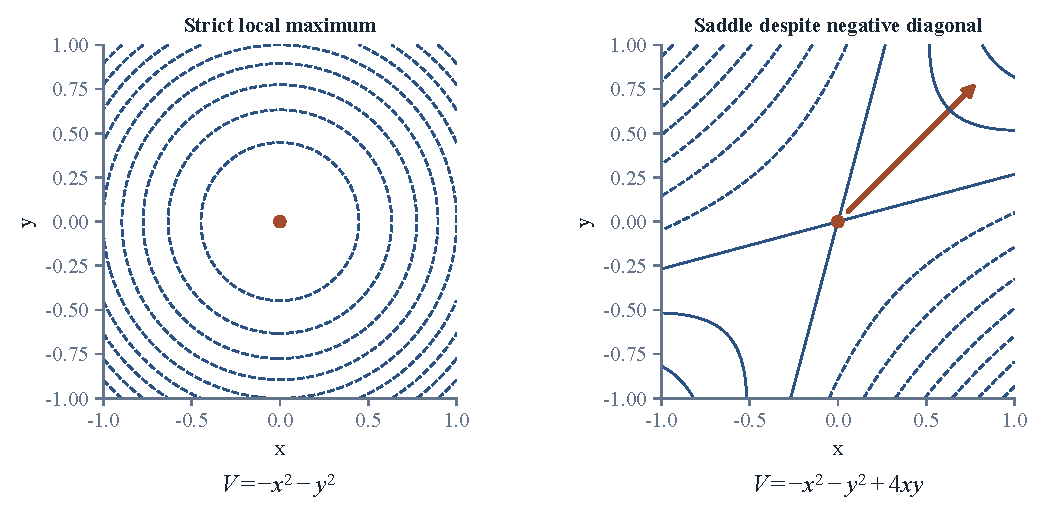
\includegraphics[width=\textwidth]{assets/hessian-directions.pdf}
\caption{Both Hessians have diagonal entries $-2$. The left Hessian is negative definite. The mixed term on the right creates eigenvalues of both signs, so the origin is a saddle and the red direction increases the score.}
\label{fig:mechanism-hessian-directions}
\end{figure}
If $V$ measures immediate satisfaction and retention, the system can reach a strong local position on those measures. Whether the position is good for users over time depends on what the objective includes and omits.

Nietzsche's “last man” supplies a literary image of satisfaction without aspiration \cite{nietzsche1883zarathustra}. The engineering account asks a different question: which valued dimensions can deteriorate without changing the score? Health, independent skill, reciprocal relationships, and public participation can all be weakly represented in a short feedback window.

Leaving a strict local maximum along a chosen path may require an initial score decline. Define the depth of that decline as
\begin{equation}
 \Delta V_{\mathrm{loss}}
 =V(x^\ast)-\min_{s\in\mathrm{path}}V(s)\geq0.
\end{equation}
The path includes the starting point. A larger value means a deeper temporary loss on that path. A universal escape barrier would additionally require optimization over admissible paths and a specified destination.

Who bears the interim loss? A service that reduces an engagement metric may lose revenue before a long-term benefit becomes measurable. A person practicing an old skill may produce less today while preserving a capability needed later. The immediate cost and delayed benefit appear on different schedules.

Changing the objective, adding constraints, creating competing services, or financing the transition can alter the path. Local optimality describes the geometry of the chosen score. Changing that score can change the way out.


\begin{figure}[ht]
\centering
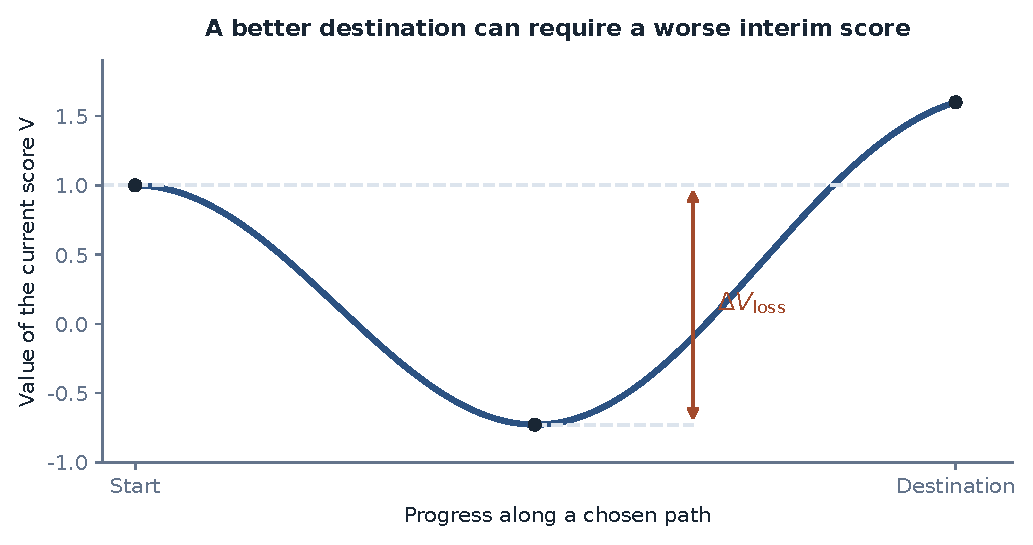
\includegraphics[width=\textwidth]{assets/escape-valley.pdf}
\caption{The temporary score loss on one chosen path is the starting value minus the minimum along that path. Including the start makes the loss nonnegative. A different objective, constraint, or feasible path can change it.}
\label{fig:mechanism-escape-valley}
\end{figure}
\subsection{Diversity as a Recovery Resource}

Many similar decisions can create a common exposure. Financial institutions using correlated models and funding structures can amplify a shock together \cite{haldane2011systemic}. Infrastructure needs alternatives that remain available after a failure; contingency standards are one way to preserve them \cite{morison2004power}.

Cultural and cognitive diversity are harder to measure but share one practical function: an alternative method can remain available when the dominant method fails. Preserving several routes consumes resources before the moment at which their value is obvious.

Recommendation systems can narrow or diversify exposure. User choices and network composition also matter. Research on cross-cutting information in Facebook showed that several mechanisms contributed, with effects that cannot be reduced to ranking alone \cite{bakshy2015exposure}. A claim about today's systems needs present measurements of today's design and use.

At the political level, Arendt's analysis emphasizes the danger of atomized people losing meaningful attachments in a common world \cite{arendt1951origins}. The useful implication is to preserve institutions in which people can participate, disagree, and obtain an answer. A platform's convenience cannot substitute for every such institution.

Automation can reduce the burden of judgment. It can also erode the practice needed for effective oversight when users become unable to evaluate a recommendation \cite{parasuraman1997humans}. The appropriate response supplies intelligible evidence, maintained skills, time, and real decision rights.

Agency survives through use and support. It needs occasions on which a person's reasons affect a process, relations in which commitments have reciprocal force, and institutions that keep objection possible. Convenience can support those conditions. Its quality should be judged by whether it does.

\section{Reconnecting the Loop}

The three collapses can reinforce one another. A weakened professional position makes immediate recognition elsewhere more attractive. A feedback environment that rarely tests judgment supplies less practice in calibration. Reduced confidence and fewer usable alternatives can make it harder to regain an effective position.

This is a possible reinforcing loop, with identifiable mechanisms and points of intervention. The book's diagnosis becomes useful when each connection can be investigated separately.

\subsection{Three Clocks, Several Interventions}

Job structures can change over years. Interfaces can change within weeks. Skills, habits, and relationships develop on varied timescales and can continue changing throughout adult life. Assigning agency recovery an immutable generational clock would obscure opportunities to improve it now.

A simple recurrence can illustrate declining entry costs into a replacement experience:
\begin{equation}
 c_{n+1}=Gc_n,\qquad
 G=g_1g_2g_3.
\end{equation}
If the $g_i$ are positive cost multipliers below one, the modeled cost decreases over repeated cycles. The recurrence describes its defined cost. It does not establish the stability, speed, or inevitability of the entire social loop.

A fuller account would need separate state variables for position, feedback, and agency, as well as delays and outside inputs. Evidence must show that one change actually strengthens the next. Those tests turn a suggestive diagram into an investigated mechanism.

Measurements can begin with narrower questions. Has entry into a profession become harder? Does assistance improve independently tested skill or only immediate output? Can users identify and challenge a consequential error? Do appeals change decisions? Are alternatives affordable and usable?

No single dashboard answers them all. Quantitative measures can be combined with longitudinal studies, task tests, institutional records, and specific cases. The possibility of gaming a measure is a reason to design review, rather than abandon measurement altogether.

\subsection{Four Functions of an Accountability System}

Consequences need a route into response. Four functions supply it:

\textbf{Discovery.} A system needs ways to detect harm, near misses, and material departures from expected behavior. Users and affected people need a reporting channel as well as operators' monitoring.

\textbf{Traceability.} Investigators need enough information to connect an event to relevant decisions, versions, configurations, and tool actions. Records should be proportionate, secure, and governed by privacy and access rules.

\textbf{Loss containment.} Someone must have usable authority to interrupt, isolate, recall, or otherwise limit continuing damage. Emergency containment may precede a full causal explanation.

\textbf{Remedy.} An affected person needs a practical route to correction, compensation where appropriate, and prevention of recurrence. Financial capacity matters because an obligation with no resources behind it may offer little relief.

These functions interact and can run concurrently. They are more demanding than a list of promised safeguards because each requires an actor, resources, and an operational interface.


\begin{figure}[ht]
\centering
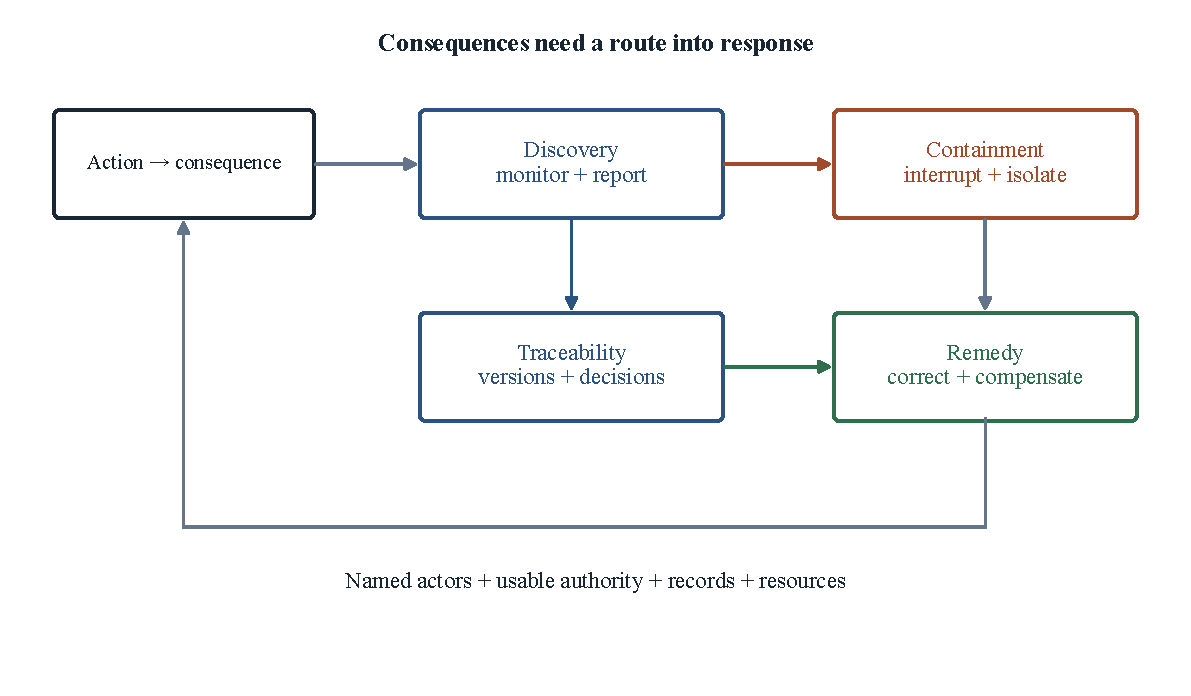
\includegraphics[width=\textwidth]{assets/accountability.pdf}
\caption{Accountability needs named actors, usable authority, records, and resources. Discovery, traceability, containment, and remedy can proceed concurrently, with their results feeding back into action.}
\label{fig:mechanism-accountability}
\end{figure}
Civil aviation is a familiar architecture in which design assurance, production controls, maintenance, operational authority, reporting, and investigation combine. Its reliability comes from aircraft and institutions together. Different domains need their own arrangements rather than a copied checklist.

Machine systems need the same clarity at their own interfaces. Which entity controls the update? Who can suspend access? Which records survive a service shutdown? Who can contest a model-based decision? Which party can fund a remedy?

Allocation can follow control, contractual role, statutory duty, or other legally established criteria. Insurance and compensation funds can pool some losses. Independent investigation can help distinguish learning from immediate fault allocation. None of these mechanisms works automatically; incentives and enforcement determine whether the promised function exists in practice.

The policy cost is visible now. The avoided harm is uncertain and later. Institutions are needed partly because the party paying for a safeguard may capture only a fraction of its benefit.

Accountability can also expand deployment. A risk with identified controls, records, and remedies is easier to evaluate than a risk that vanishes into a chain of disclaimers. Some uncertainty becomes manageable because the system now knows what it will do when uncertainty becomes consequence.

\subsection{Judgment Needs Standing}

Three decisions remain central: which consequences are acceptable, how much evidence is enough to proceed, and who may impose a cost on whom.

Models can inform all three. They can estimate outcomes, compare options, reveal inconsistencies, and help people articulate positions. Technical competence alone does not supply the right to decide.

The normative principle advanced here is that people bearing consequences must retain effective voice, representation, and access to challenge. Direct exposure is one source of standing; lawful delegation, professional duty, democratic authorization, and protections for absent or vulnerable parties are others.

A judge's, clinician's, or juror's authority depends on an institutional role and duties owed to others. The responsibility of a professional and the bodily risk borne by a patient remain distinct.

Jury systems illustrate one institutional choice about participation and judgment \cite{kalven1966american}. Their justification rests on the role, procedure, and distribution of public power. Medical consent illustrates another: expertise informs the options while the patient retains rights over exposure. Aviation assigns operational authority through defined roles, competence, and duties.

The common achievement is a decision with an intelligible basis, a recognized scope, and a place where it can be questioned. An opaque recommendation becomes a legitimate decision only through such an arrangement.

\subsection{A Person's Worth Survives a Falling Production Cost}

A society that values people only through scarce output becomes vulnerable when output becomes abundant. It needs a richer account of participation, care, relationship, judgment, and finite life.

The fact that a consequence happens to fall on someone does not justify making them bear it. Exposure creates a claim to protection and voice, rather than a duty to suffer for meaning. Responsibility should follow a justified allocation of authority and control.

Some parts of life remain personal in a direct sense. Another person can advise, work, or decide on one's behalf. They cannot thereby live the same finite life or occupy the same relation. Assistance changes what a person can do; it does not make the person's stake disappear.

The chapter's repair is therefore structural and concrete. Rebuild routes into useful contribution. Preserve feedback that can correct a claim. Keep exit, objection, and meaningful commitments available. Attach consequential action to people and institutions able to answer for it.

These choices create costs. The next chapter asks how to distinguish the costs that merely obstruct from those that preserve the conditions under which progress remains worth having.

\chapter{Rebuilding Value in the Shear Zone}

When a capability becomes cheap to obtain, the social position once attached to it can move. The destination depends on demand, ownership, bargaining power, and public institutions. Three things must be kept distinct: a function's social necessity, the reward given to whoever performs it, and the dignity of the person involved.

Verification, care, sustained relationships, and responsibility can become relatively scarce in a world of abundant generation. Turning that scarcity into support and recognition requires arrangements that can pay for it.

\section{A History of Capabilities Leaving the Body}

\subsection{Writing Changed What Memory Proved}

In Plato's account, Socrates worries that writing can supply the appearance of wisdom without its internal possession. A stored statement can be consulted without the learner acquiring the judgment behind it.

The concern identifies a recurring distinction. External storage changes what a person's immediate performance demonstrates. It also creates new kinds of thought: a written proof can be paused, checked, and challenged by someone who never met its author.

Oral tradition itself was more inventive than a storage metaphor suggests. Parry and Lord's work on epic singers described composition through reusable patterns and formulas, with performances varying rather than reproducing one fixed text \cite{parry1971making,parry1960singer}. Writing changes a practice of memory and composition, not merely the location of a recording.

Modern experiments on expected access to information show another reallocation: remembering where to retrieve material can improve while memory for the material changes \cite{sparrow2011google}. External memory can support a stronger system when the person retains enough internal knowledge to recognize relevance, error, and missing context.

The migration is from holding every item to knowing how to use and assess what remains accessible. Access itself still depends on records, preservation, tools, and institutions.

\subsection{Cheap Copies Changed Authority}

Printing lowered the cost of reproducing texts and helped reorganize correction, comparison, distribution, and controversy \cite{eisenstein1979printing}. It expanded audiences and created work around editions, interpretation, and trust.

The history is uneven across regions and technologies. Movable type in Europe was one important transformation within a much longer history of writing and printing. The point is the changing relation between possession and authority.

When access to a text becomes easier, ownership of a copy supplies less distinction. A dependable edition, a persuasive interpretation, or a trusted publisher can become more valuable. Cheap copying can spread errors along with corrections.

Computer systems extended the movement to rule execution. Calculation, sorting, accounts, retrieval, and repeatable workflows moved into machinery. A professional's position could shift toward choosing the model, interpreting exceptions, checking the result, and assuming a defined responsibility.

Such shifts create winners, losses, and new dependencies. They do not conserve the number of jobs or the value of every old skill. Institutions help determine whether the increased productive capacity becomes broadly shared benefit.

\subsection{Clocks and Engines Reorganized the Operator}

A mechanical clock made intervals publicly comparable and helped support schedules that could be imposed across workers and machines. The resulting coordination expanded productive possibilities while changing control over the working day.

Steam power moved large quantities of work into fuel, engines, factories, and transport networks \cite{landes1969unbound}. Human muscle remained necessary in many tasks, yet it was no longer the only scalable source of industrial power.

The operator's problem changed. Keeping machines, fuel, schedules, and people coordinated could become more important than supplying the direct force. The new positions depended on access to capital, education, authority, and organization.

These histories expose a repeated pattern: technology changes which evidence a society uses to recognize competence, and which institution controls the next scarce interface.

\subsection{Formal Discovery Is Moving Too}

Machine learning has reached language, code, design, scientific hypotheses, and mathematical search. The artifact once treated as evidence of years of preparation can now be produced through a different route.

Mathematics is a demanding case because discovery and checking can be distinguished sharply. AlphaGeometry's 2024 work combined neural proposals with symbolic deduction \cite{trinh2024alphageometry}. In May 2026, an OpenAI-generated construction challenged the conjectured near-linear exponent for the planar unit-distance problem; a group of mathematicians supplied a concise exposition and analysis \cite{alon2026remarks}.

The intellectual contribution is substantial. It changes which problems are worth asking and which techniques can be combined. The knowledge still includes the precise statement, its proof, its relation to earlier work, and the consequences other researchers can extract.

September's OpenAI announcement on Navier--Stokes went further, presenting a smooth-forcing finite-time singularity construction and a Lean formalization \cite{openai2026navierstokes}. The theorem's domain, force assumptions, and correspondence to the stated problem are central parts of evaluating it. “The model solved fluids” would discard the very content that makes the result mathematical.

The current lesson is that verification itself can accelerate. Formal tools can check derivations cheaply once an adequate statement and proof exist. The remaining human and institutional work includes specification, understanding, review, priority, pedagogy, and choosing what deserves attention.

Tao's evolving account of AI-assisted mathematics emphasizes these distinctions between candidate production, independent checking, formalization, and understanding \cite{tao2026aiviews}. The scarce interface can move again when a previously laborious checking step becomes automated.

An illustrative capacity ratio is
\begin{equation}
 \rho=\min\left\{1,\frac{d}{g}\right\},
\end{equation}
where $g$ is candidate production and $d$ comparable digestion or review capacity, in matching units. In the unsaturated region $0<d/g<1$, $\rho$ falls when $g$ grows proportionally faster than $d$. At the capped value one, the same strict derivative statement need not hold.

The quantity is useful only after defining what counts as a candidate and what digestion requires. Reviewing a formal proof, understanding it, and integrating it into a research field are different activities.

\subsection{Capability, Qualification, and Permission}

Embodied action and biological intervention extend the same change into heavier media. A generated policy needs an actuator and an operating domain. A proposed sequence needs a biological process capable of using it. A demonstrated capability needs an account of where it can be relied upon.

Traditional qualifications bundled several signals: preparation, experience, exclusivity, and responsibility. Spence's signaling framework helps explain how some qualifications communicate information under particular incentive conditions \cite{spence1973job}. Machine assistance can loosen the bundle.

The response should inspect each function. Does the assessment establish the skill needed? Does the trainee still obtain the experience needed for later judgment? Does the professional have authority matching their duty? Does the user know which part of a result was actually checked?

The history offers no automatic promise that value migrates fairly. It offers a practical method: identify the capability being externalized, the old signal losing force, and the new interface on which reliable performance depends.

The next four principles ask how those interfaces should be maintained.

\section{First Principle: Keep the Feedback That Gives a Boundary Shape}

A boundary is useful when it permits the right exchanges and resists the wrong ones. A cell membrane, a professional role, and a person's commitments differ greatly, yet each depends on a distinction that has to survive contact.

The chapter calls this a \emph{damping ontology}: understand a practical boundary partly through how it receives, limits, and answers disturbance. The phrase brings attention to interaction. It supplies no single physical law for membranes, identities, and institutions.

\subsection{A Boundary Has to Be Maintained}

An illustrative balance writes
\begin{equation}
 \dot B=-\frac{B}{\tau}+P.
\end{equation}
$B$ is a defined measure of a maintained capability or boundary, $\tau$ its decay timescale in this model, and $P$ the supporting input per unit time. With constant $P$ and positive $\tau$, the balance tends toward $B^\ast=P\tau$.

The equation describes a mechanism to test. Some boundaries persist passively; others need substantial continuing work. Psychological or institutional variables must be defined and measured before this model can explain their change.

Living systems offer a concrete maintenance account. Recognition, tolerance, repair, and controlled exchange preserve an organism's functioning \cite{burnet1959clonal}. An immune system's distinction is more elaborate than a simple self/nonself label, and neither all mistakes nor all changes are fatal.

Human boundaries develop through relationships, action, learning, and institutions. A disagreement can make a preference explicit. Keeping a promise can establish reliability. A usable right of refusal can keep a relation voluntary. These interactions need continuity and response.

The functional aim is selective exchange. A sealed wall and an unprotected opening are both poor models of a capable living boundary.

\subsection{Why Some Signals Need a Stake}

Zahavi's handicap account and later signaling models explain how different costs can support honest distinctions \cite{zahavi1975mate,grafen1990biological}. A simple separating case is
\begin{equation}
 c(q_{\mathrm{low}})>b>c(q_{\mathrm{high}}),
\end{equation}
where $b$ is a benefit and $c(q)$ the cost of sending a signal for type $q$. Under the model's incentive assumptions, the higher type benefits from signaling while the lower type does not.

The relation between cost, benefit, type, and possible deception does the work. A signal need not always impose a large equilibrium cost to remain informative; direct indices, aligned interests, enforcement, and differential incentives can also sustain honesty.

This precision matters when AI makes polished artifacts cheap. An article, portfolio, or résumé may reveal less about an individual's unaided production skill. It can still reveal choice, judgment, taste, or effective use of a tool if the assessment is designed around those properties.

Three kinds of evidence deserve particular attention. A traceable history can be harder to fabricate than a claim about history. Task-specific demonstration can establish a capability more directly than an attractive sample. An enforceable stake can give an assertion consequences for the party making it.

Time contributes when the property itself develops or is observed over time. Sustained reliability requires repeated opportunities to behave reliably. Skill formation may require practice and recovery. Better training can reduce unnecessary delay, so “it takes time” should identify the relevant learning or biological process.

An expensive ordeal that measures little is a poor signal. A cheap test that directly establishes the desired capability can be an improvement.

\subsection{Formation and Maintenance Are Different Bills}

A skill must be acquired and then preserved. A record must be created and then kept readable. A relationship must begin and then continue. Creation cost and maintenance cost can move independently.

Thermodynamics gives a precise balance for a physical open system:
\begin{equation}
 \frac{\mathrm d S_{\mathrm{sys}}}{\mathrm dt}
 =\dot S_{\mathrm{prod}}+\dot S_{\mathrm{flow}},
 \qquad \dot S_{\mathrm{prod}}\geq0.
\end{equation}
Entropy has units $\mathrm{J\,K^{-1}}$ and the rates $\mathrm{J\,K^{-1}\,s^{-1}}$. A steady internal entropy requires outward entropy flow to balance internal production under the specified boundary and sign convention.

Schrödinger's discussion of life and the work on dissipative structures make the physical maintenance problem vivid \cite{schrodinger1944,nicolis1977,prigogine1977nobel}. A social practice also needs a maintenance account, but its trust or meaning cannot simply be inserted as thermodynamic entropy.

A library survives through storage, cataloging, migration, interpretation, and use. A standard survives through implementation, revision, and institutions willing to resolve disputes. The important commonality is a continuing chain of support.

Artificial tools can lower both formation and maintenance costs. They can recover a damaged text, translate it, check references, and help new readers enter a field. The result depends on whether the necessary functions remain funded and performed.

Cost does not determine worth. A costly institution can preserve something harmful; a nearly effortless act can matter deeply. The normative question is what should be maintained, for whom, and at whose expense.

The first principle is consequently functional: preserve feedback, practice, records, and enforceable commitments where they sustain a valued capability or boundary. Improve the means whenever the same function can be supplied at lower cost.

\section{Second Principle: Keep the Standard Open to Correction}

An optimizer needs a way to compare alternatives. Choosing that comparison already makes decisions about value.

\subsection{A Score Contains a Settlement}

Suppose a proposal $\mathbf x$ has normalized evaluations $v_j(\mathbf x)$ on $m$ dimensions. A weighted score is
\begin{equation}
 U(\mathbf x)=\sum_{j=1}^{m}w_jv_j(\mathbf x),
 \qquad w_j\geq0,\quad\sum_jw_j=1.
\end{equation}
The score makes a tradeoff operational. It also places part of the dispute inside the weights, normalization, and functional form.

Two proposals can have the same score and quite different effects. A dimension with zero weight can change without affecting the objective. A weighted sum allows some losses to be offset by gains elsewhere. Hard constraints, priorities, or other decision rules may be more appropriate for requirements that should not be traded that way.

In a nonconvex multiobjective problem, varying positive linear weights can miss unsupported Pareto-efficient points \cite{das1997closer}. The chosen scalarization therefore affects which alternatives can emerge from the search. Keeping the original dimensions visible allows reviewers to inspect the omission.


\begin{figure}[ht]
\centering
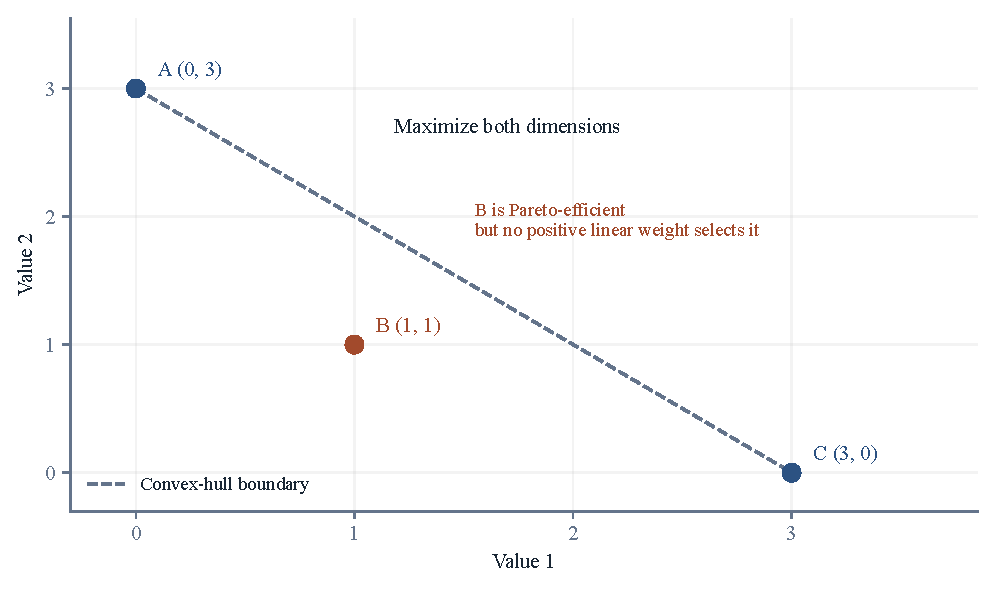
\includegraphics[width=\textwidth]{assets/unsupported-pareto.pdf}
\caption{The feasible set is $A=(0,3)$, $B=(1,1)$, and $C=(3,0)$, with both dimensions maximized. $B$ is nondominated. Yet $\max\{3w,3(1-w)\}\geq1.5>1$ for $0\leq w\leq1$, so no linear weighting selects $B$.}
\label{fig:mechanism-unsupported-pareto}
\end{figure}
Social aggregation adds another set of conditions. Arrow's theorem identifies incompatible requirements for a social ordering under an unrestricted preference domain with at least three alternatives \cite{arrow1951social}. Gibbard and Satterthwaite identify strong restrictions on deterministic strategy-proof choice under their respective assumptions \cite{gibbard1973manipulation,satterthwaite1975strategy}.

The theorems clarify tradeoffs in institutional design. They leave room for restricted domains, other information, different procedures, and explicit compromises. Their assumptions identify which institutional tradeoffs must be made explicit.

No-free-lunch results likewise concern averaging over specified spaces of objective functions \cite{wolpert1997no}. Real systems succeed by exploiting structure in particular task distributions. Representation, data, and objectives carry those commitments into deployment.

When a proxy becomes a target, optimization can exploit the gap. A game agent can collect reward without completing the intended task \cite{amodei2016concrete}. An organization can improve reported output while weakening the service the report was meant to describe.

The response is to expose the settlement: retain underlying measures, investigate gaming, permit challenge, and revise the objective when the proxy fails.

\subsection{What Formal Limits Establish}

Gödel's incompleteness theorems, Turing's undecidability result, Tarski's undefinability result, and Rice's theorem locate different boundaries \cite{godel1931,turing1936,tarski1936wahrheitsbegriff,rice1953classes}. They are strong precisely because their objects and conditions are explicit.

A sufficiently strong, consistent, effectively axiomatized arithmetic theory has undecidable sentences. Under the usual conditions it cannot establish its own formalized consistency. A universal program cannot decide the halting of every arbitrary program. A suitable arithmetic language cannot define its own complete truth predicate in the required sense. Nontrivial extensional properties of partial computable functions are undecidable in general.

Arguments about human cognition and machine authority require additional premises. Lucas and Penrose's arguments about minds and formal systems involve additional assumptions about human and machine reasoning \cite{lucas1961minds,penrose1989emperor}.

The relevant engineering practice is to state which assumptions a guarantee uses. A proof connects an implementation to a formal specification. Requirement analysis and evidence connect that specification to a desired use. Authority and rights connect the use to an acceptable decision.

The seL4 work made important parts of the first relation machine-checkable while listing what remained assumed \cite{klein2009sel4}. A smaller trusted base improves inspectability. Questions beyond the formal specification still need their own evidence and judgment.

Static analysis illustrates the choice. Let $B$ be programs with a target property and $L$ programs reported by a tool. Then
\begin{equation}
 B\subseteq L\quad\text{means no missed positives},
 \qquad
 L\subseteq B\quad\text{means no false positives}.
\end{equation}
A terminating universal tool satisfying both for a Rice-type property would be a forbidden general decision procedure. Restricting the language or property can permit exact decisions; sound approximation, runtime monitoring, and review offer other useful arrangements.

Specific progress remains possible within general limits. The 2024 busy-beaver project established the five-state value $47{,}176{,}870$ through collaborative computation and proof work \cite{bbchallenge2024}. Undecidability of the unrestricted function did not settle that particular case.

\subsection{Evidence, Authority, and Revision}

A standard can be proposed by a person or machine, tested by software, challenged by evidence, and authorized through an institution. The legitimacy of adopting it depends on the relevant rights and procedures.

The normative requirement advanced here is openness to correction. People affected by a consequential decision need a way to learn its basis, challenge a relevant error, and seek a remedy. Experts need ways to revise a standard when the world exposes a failure.

The stakes and distribution of power supply the case for this principle. Its justification belongs in the open, alongside the technical evidence.

\subsection{Where Scarcity May Move}

If routine production becomes cheaper, some complementary functions can become more important: reliable verification, well-supported care, field judgment, long-term education, and institutions able to resolve consequential disputes.

Each has a different constraint. Verification needs evidence appropriate to a claim. Care needs time, skill, access, and sometimes a particular relationship. Field judgment needs information and an effective action position. Education needs a path by which learners develop capabilities rather than merely submit outputs.

These functions offer candidates for investment. Parts of each function can improve through tools. The useful criterion is which necessary function remains difficult to supply at the required quality.

Scarcity also fails to guarantee high pay. A caregiver's bargaining power, a public budget, or a family's income can matter more than the activity's necessity. Productivity differences can raise relative service costs without automatically raising the worker's reward.

The second principle therefore has two parts. Keep the chosen standard open to evidence and challenge. Then examine whether the people maintaining its necessary functions actually receive the resources and authority the function requires.

\section{Third Principle: Divide the Work Without Hiding the Bill}

A powerful search system can move quickly through possibilities. A trusted professional role takes time and institutions to establish. One is a readily callable capability; the other is a position from which a judgment can carry authority and obligation.

The book's kinetic--potential image distinguishes movement from position. It is a metaphor for complementary functions, not a conversion between computational ability and moral energy.

\subsection{Fast Capability, Slowly Formed Standing}

Lifting one kilogram by one meter near Earth's surface increases gravitational potential energy by about $9.8\,\mathrm J$. Doing it faster changes the power needed. The destination and the rate of getting there are different properties.

For comparison, an idealized unbiased bit reset near room temperature has a Landauer bound of about $2.9\times10^{-21}\,\mathrm J$. Their ratio is on the order of $3\times10^{21}$. This compares one macroscopic lift with one ideal bit reset. Actual inference contains many operations and substantial hardware overhead; the ratio cannot price an AI task.

The valid lesson is the separate ledger. Symbol processing and physical work can have very different marginal costs, while both remain physical. A model can propose thousands of paths without lifting the load along each one.

Standing has another preparation. A judge's office, a clinician's responsibilities, or a laboratory's recognized competence exists through qualifications, records, procedures, and authority. A model can improve the judgment made there. Its speed does not automatically confer the role.

The division need not remain fixed. Some routine decisions can be delegated through established rules. Some checking can become fully automatic. The authority to delegate, the conditions of delegation, and responsibility for its effects must still be identified.

\subsection{The Objective Is Part of the Design}

An optimization can be written
\begin{equation}
 x^\ast\in\arg\max_{x\in\mathcal X} f(x).
\end{equation}
Using membership allows multiple maximizers; in some problems the maximum is not attained. The feasible set $\mathcal X$ and objective $f$ carry choices about what counts and what is permitted.

A search engine can help inspect and revise both. It can reveal an inconsistency, estimate a consequence, or identify an alternative. The social decision is which constraints and priorities have a legitimate claim on the resulting action.

This is the practical content of symbiosis. Human and machine functions connect through explicit standards, evidence, and authority. Capability expands the available routes; institutions determine which routes may impose which burdens.

The arrangement can fail in either direction. A capable system can be blocked by rules that protect no useful function. A weak decision structure can give an optimizer broad authority without an adequate account of whose objective it is advancing.

The design task is to improve the whole route from problem to consequence.

\subsection{Which Friction Earns Its Place?}

Friction should be evaluated by what it produces.

Some friction is pure process loss: duplicate entry, incompatible formats, unnecessary waiting, avoidable transport, or a requirement whose original purpose has disappeared.

Some forms a capability: practice, repeated observation, recovery, and the experience needed to distinguish ordinary cases from exceptions.

Some protects an interest: consent, independent verification, a safe operating limit, an appeal, or an opportunity to stop before an irreversible step.

Some extracts a rent: an artificial bottleneck, an exclusionary credential, or complexity maintained because someone profits from being the only interpreter.

The categories require investigation. An approval may protect a real interest and still have an inefficient procedure. A credential may establish competence and also exclude people unfairly. Improving the mechanism can preserve the function while reducing cost.

\begin{table}[ht]
\centering\small
\begin{tabularx}{\textwidth}{@{}lYY@{}}
\toprule
Friction & What to ask & Productive response\\
\midrule
Process loss & Which valued result would disappear if this step vanished? & Remove or simplify the step when no result depends on it.\\
Capability formation & What learning or recovery occurs here? & Improve practice and test transfer.\\
Protection & Whose interest does this preserve, and does it work? & Keep the function; compare cheaper implementations.\\
Rent or exclusion & Who benefits from the barrier itself? & Challenge the allocation and redesign access.\\
\bottomrule
\end{tabularx}
\caption{The function of a delay or barrier matters more than its size.}
\end{table}

A useful refusal, a well-designed test, and an effective consent process often make later action easier by making it defensible. Their costs belong in the project's enabling infrastructure.

The third principle is to use automation to remove losses and strengthen necessary functions. The point of preserving a boundary is that more can safely and legitimately pass through it.

\section{Fourth Principle: Revise the Loop That Revises the Work}

A decision changes the environment. New evidence changes the standard. A changed standard alters the next decision. Improvement therefore includes the procedure used to judge improvement.

\subsection{A Recursive Process Can Learn or Drift}

For a scalar iteration,
\begin{equation}
 x_{n+1}=g(x_n),
\end{equation}
a continuously differentiable map with a fixed point $x^\ast$ is locally attracting when $|g'(x^\ast)|<1$. In several dimensions, the Jacobian's eigenvalues govern the corresponding local result under the usual regularity assumptions.

An institution updating its evaluation rules is more complicated. Objectives, participants, evidence, and external conditions can all change. The equation supplies a reason to inspect the update rule, rather than a promise of convergence.

The useful question is whether a revision preserves learning. Can errors be identified? Can affected people challenge the interpretation? Is there enough continuity to distinguish a better rule from a lucky outcome?

\subsection{Keep Some Practice Inside the Person}

Assistance can make a task cheaper while moving practice elsewhere. A person who wants to retain a capability needs some occasions to exercise it and obtain interpretable feedback.

Choose the capability first. Someone preserving spatial judgment might sometimes navigate without turn-by-turn instructions. Someone learning a language might draft a passage before requesting corrections. Someone responsible for code should retain the ability to read, test, and explain the parts they will maintain.

The useful unit is the learning loop, rather than unaided effort for its own sake. A good tutor, simulator, or assistant can improve that loop. Deliberately withholding an effective aid is worthwhile only when it serves a defined purpose.

Defaults can protect practice without requiring a fresh contest of will at every moment. A regular session, a shared commitment, or a tool configuration can make a desired activity ordinary. Waiting can preserve a decision point; feedback can be delayed when immediate scoring distorts the activity.

Different people have different resources. Time, disability, care responsibilities, money, and fatigue change which arrangements are feasible. Assistance often expands agency most for people facing the highest barriers. Preserving a skill should not become a demand that everyone accept the same avoidable burden.

Organizations influence the available choices. A worker cannot preserve every valuable learning process in unpaid hours while being evaluated only on immediate output. Training, staffing, and assessment have to carry part of the cost.

\subsection{Build Organizations That Produce Warrants}

A laboratory, hospital, engineering firm, court, auditor, or certification body can produce a judgment that others are entitled to rely on. Its product is partly a warrant: a result connected to evidence, procedure, expertise, and responsibility.

The name alone supplies none of this. An approval chain can generate signatures without generating confidence. An audit can become a ritual. A university can reward output volume while neglecting understanding.

Three conditions make checking substantive. Reviewers need access to relevant original evidence. Their incentives must allow an unfavorable finding. Their authority must be strong enough to change the proposed action.

Tools can accelerate each part. They can organize evidence, check consistency, reproduce calculations, and highlight anomalies. A trustworthy organization captures those gains while examining the new failure modes introduced by the tools.

Four slow assets deserve deliberate support: informative exposure over time, a record of trustworthy behavior, a clear distribution of duties, and the independence needed to challenge a profitable error.

The timescales vary. Some checks can be automated almost completely. Some clinical or material observations require time to pass. An organization should distinguish a queue caused by poor administration from a follow-up period that supplies necessary information.

Markets can reward dependable judgment, but information asymmetry, delayed consequences, and shared benefits can leave safeguards underprovided. Public standards, professional norms, procurement, liability, and independent institutions can change those incentives.

An organization that invests in reliability may also save money by preventing rework and incidents. The cost is not necessarily a permanent handicap. The comparison must include the losses the faster-looking arrangement produces later.

Records connect the periods. A finding should remain traceable after staff turnover or a model update. A failed prediction should enter the next review rather than disappear behind a new version.

\subsection{A Life Has More Than One Axis}

Output is measurable and often useful. It is an incomplete account of a person's life.

National accounts measure defined economic aggregates. They do not claim to measure every form of worth. Trouble begins when a convenient output measure becomes the sole basis for recognizing activity.

AARP's March 2026 report estimates that unpaid adult caregiving in the United States supplied 49.5 billion hours in 2024, with an imputed economic value of about \$1.01 trillion \cite{aarp2026valuing}. The valuation uses a method and wage assumptions; it is not money actually paid. The report also changed aspects of its method, so simple comparisons with older headline totals can mislead.

The estimate makes visible work already occurring. It also exposes the difference between being socially necessary and having a funded position.

Function and experience are separate evaluative dimensions. A highly productive activity can leave a person depleted. An activity with modest market output can sustain a valuable relationship or a meaningful experience. Calling the dimensions separate does not establish statistical independence between them.

The same person can value both. Automation can free time, improve access, and remove drudgery. The benefit becomes part of a good life through what the person can then do, experience, and sustain.

This is why productivity need not be defended by finding ever more output to assign to everyone. A society can use increased capacity to support care, education, leisure, participation, and a more secure floor beneath choice.

The fourth principle is to keep revising the arrangement by its actual consequences. Preserve learning, use tools to improve evidence, fund the necessary slow work, and evaluate lives on more than one axis.

\section{A Constitution for a More Capable Civilization}

The four principles concern boundaries, correction, division of work, and continuing revision. At a larger scale, they ask where a civilization will direct the capacity it has gained.

\subsection{Keep a Frontier That Answers Back}

Some problems compel sustained contact with material limits: deep-space missions, ocean engineering, ecological restoration, fundamental experiments, infrastructure renewal, and the formation of capable people.

They demand resources, time, and coordination. A useful shorthand for projects with high requirements on all three coordinates is
\begin{equation}
 \mathcal F=
 \{(R,T,G):R\geq R_\ast,\ T\geq T_\ast,\ G\geq G_\ast\}.
\end{equation}
This defines the intersection chosen by those thresholds. A broader class of difficult projects may be high in only one or two coordinates.

What makes such projects worth doing is their benefit, knowledge, or protection of future possibilities. Their resistance ensures that a convincing description cannot substitute for the required result.

A spacecraft needs an actual trajectory and reliable systems. An ocean instrument needs to survive pressure and corrosion. An ecosystem intervention needs observations through changing seasons and responses. A new scientific claim may need an instrument that does not yet exist.

Feedback is often costly and delayed in these settings. That can make evidence sparse rather than unusually dense. A well-designed program buys discriminating tests, preserves failure records, and stages commitments so uncertainty can be reduced before the largest exposures.

AI can improve design, analysis, and coordination across these frontiers. The ambition is to obtain more knowledge and service from each costly contact. Calling a problem “physical” does not make its current method optimal.

Long projects need a public account of opportunity cost. Resources directed toward a mission are unavailable elsewhere. Current decision-makers must explain what future benefit they expect, who bears the interim burden, and how later participants can revise the commitment.

Some benefits are shared or delayed enough that individual investors will not fund the socially useful amount. Public institutions, cooperative arrangements, and long-lived funds can carry the account across those periods.

\subsection{Life, Mind, and Trust as Areas of Growing Demand}

Three domains concentrate needs that cheap generation alone does not meet: maintaining bodies, supporting mental and relational life, and establishing dependable judgments.

Biotechnology can change what is treatable. Programmable genome editing supplied a major mechanism \cite{jinek2012programmable}. Clinical delivery, safety, access, and long-term evidence determine which benefits reach people. The 2026 Casgevy record is one current example of progress joined to continued obligations \cite{fda2026casgevy}.

Mental health requires similarly careful boundaries. WHO's updated 2025 report describes more than a billion people living with mental disorders and substantial gaps in services \cite{who2025mental}. A conversational interface may provide useful support. Clinical effectiveness, safety, escalation, privacy, and access need evidence appropriate to the service advertised.

Trust becomes a technical and institutional product when convincing signals are cheap. Provenance, secure identity, independent checking, and enforceable responsibility can help reconnect claims to their origins and consequences. C2PA illustrates a defined technical contribution, with its validation scope made explicit \cite{c2pa2026spec}.

These needs can expand industries. They can also remain poorly paid or unavailable to people who need them most. A demand forecast does not supply a distribution system.

Baumol's mechanism clarifies one possible relative-price pressure \cite{baumol1967macro}. If the progressive sector's productivity grows at constant rate $r$, the slower sector's does not, and wages move together under the model, then a relative unit-cost index can evolve as
\begin{equation}
 \frac{C_{\mathrm{slow}}(t)}{C_{\mathrm{fast}}(t)}
 =
 \frac{C_{\mathrm{slow}}(0)}{C_{\mathrm{fast}}(0)}
 e^{rt}.
\end{equation}
The sector outputs must be consistently indexed; they are not literally the same product. Different productivity, wage, capital, and service-quality paths change the result.

Rising relative costs can generate investment, shortages, unpaid family burdens, or exclusion. Public payment, insurance, labor institutions, and service design influence which outcome occurs.

\subsection{The Gaia Hypothesis as a Design Question}

A more speculative possibility follows from coupling industrial and biological systems: could a civilization develop stronger capacities to maintain, repair, and reproduce its material basis?

Von Neumann's self-reproducing automata separated a description from machinery able to use and copy it within a formal construction \cite{vonneumann1966theory}. Biological replication adds actual materials, energy, error correction, and selection. Engineering reproduction depends on supply chains whose independence has to be demonstrated.

Self-maintenance, reproduction, and heritable variation are useful properties to inspect. Their presence at some scale does not establish that the entire planet is one organism or that an industrial network can reproduce autonomously from raw resources.

Copy fidelity gives one measurable constraint. With independent per-site error probability $\nu$ over length $\lambda$,
\begin{equation}
 Q=(1-\nu)^\lambda\approx e^{-\nu\lambda}.
\end{equation}
The approximation requires small per-site error, with accumulated higher-order terms negligible at the desired accuracy. Selection, repair, redundancy, and the effects of particular mutations determine what information persists \cite{kunkel2000dna,gilbert1986}.

Circular material use provides another measure. For a defined material, boundary, and period,
\begin{equation}
 \kappa_{\mathrm{mat}}=
 \frac{\dot m_{\mathrm{returned\ to\ usable\ supply}}}
      {\dot m_{\mathrm{total\ usable\ input}}}.
\end{equation}
The numerator must be part of the denominator for the fraction to lie between zero and one. Stocks, delays, material quality, and repeated counting need explicit treatment.

A high recycling share can reduce demand for new extraction. It does not establish energetic self-sufficiency, complete reproduction, or ecological stability. Recycling uses energy, loses or disperses some material, and may change quality. An open system still needs energy throughput and entropy export.

“Gaia” is useful here as a question about coupled self-maintenance. It provides no guarantee that the maintained state would favor humans. A stable planetary process can be hostile to a particular species.

The engineering frontier is consequently specific: improve repair, circularity, resource resilience, and compatible ecological relations while preserving control over the consequences. A self-maintaining subsystem may be easier to sustain and harder to stop once dispersed. Both belong in its evaluation.

\subsection{Four Commitments}

A practical constitution for this setting can begin with four commitments.

\textbf{Keep correction possible.} Evidence, appeal, revision, and interruption must remain available as capability grows.

\textbf{Give affected people a voice in the cost.} Exposure should bring information, representation, and remedies, especially where burdens can be exported.

\textbf{Preserve necessary functions while improving their means.} Learning, verification, consent, recovery, and responsibility should survive the removal of waste.

\textbf{Evaluate the whole consequence over the relevant time.} A fast interface should not claim a gain whose bill sits in an unobserved body, network, or future.

Silicon--carbon symbiosis names one possible arrangement of these commitments. It is a shorthand for complementary capabilities and stakes, not a permanent division based on the periodic table. Digital systems remain material; living people also learn, compute, copy, and delegate.

The desired arrangement lets powerful tools expand human and ecological possibilities while keeping the consequences governable. It has to be built through standards, incentives, evidence, rights, and resources.

The final chapter tests the framework against two extremes: systems that reproduce their own physical basis, and systems that seem to replace physical life with representation. Both return to the same question: what must keep running for the possibility to remain real?

\chapter{Freedom Inside the Constraints}

A system that builds the next instance of itself seems to offer a way around the manufacturing bottleneck. A simulated world seems to offer a way around the burden of physical experience. Both are useful stress tests for the book's argument. Where do resources, time, and coupling go when the apparent route becomes so much lighter?

\section{Replication, Irreversibility, and the Substrate}

\subsection{What Self-Replication Changes}

Compare a fixed production line with an idealized population that doubles at a constant interval:
\begin{equation}
 N_{\mathrm{line}}(t)=1+\frac{t}{\tau_{\mathrm{line}}},
 \qquad
 N_{\mathrm{rep}}(t)=2^{t/\tau_{\mathrm{rep}}}.
\end{equation}
The quantities are unit counts relative to the stated starting condition. The first assumes fixed capacity; the second assumes adequate inputs and an unchanged doubling time. A manufacturing system can add capacity, and a replicating system can encounter limits. The assumptions define the comparison.

Replication can distribute construction. It still needs feedstock, energy, space, transport, error control, and waste handling. The next producer is also something that must be built and maintained.

The resource barrier becomes an uptake problem: what can be extracted or obtained from the environment at the required rate? The temporal constraint includes the cycle of acquisition, construction, maturation, and copying. The topology includes access to suitable environments and pathways of spread.

None of these is intrinsically faster than every manufacturing process. Biological replication can be fast for a microbe and slow for a tree. An engineered replicator's rate would depend on what it must reproduce and the environment it assumes.

Von Neumann's formal construction demonstrated a way to separate a description, its copying, and its use by a constructor \cite{vonneumann1966theory}. Physical implementation adds a full industrial and thermodynamic account. A printer making one of its own parts is a useful step toward automation; it is not yet an autonomous system rebuilding its entire supply basis.

The governance problem changes when production is dispersed beyond a few facilities. Monitoring spread, limiting access to necessary conditions, and preserving effective intervention points can become more important. Their effectiveness must be established for the particular system.

The ratio
\begin{equation}
 \chi=\frac{\tau_{\mathrm{assessment}}}
            {\tau_{\mathrm{doubling}}}
\end{equation}
identifies one timing pressure. Under continued ideal doubling, assessment lasting $\chi$ doubling times permits a factor $2^\chi$ increase before completion. A large ratio can make delayed recognition costly. Containment, access, detection quality, and intervention strength still determine whether control is possible.

\subsection{Growth Can Settle, Oscillate, or Overshoot}

Exponential growth cannot continue indefinitely in a finite environment. Its eventual form depends on the feedback.

A delayed logistic model illustrates the difference:
\begin{equation}
 \frac{\mathrm dN}{\mathrm dt}
 =rN(t)\left(1-\frac{N(t-\theta)}{K}\right).
\end{equation}
$r>0$ is a growth rate, $K>0$ a fixed capacity, and $\theta$ a feedback delay. The state requires an initial history over the delay interval.

Linearizing around the positive equilibrium $N=K$ gives
\begin{equation}
 \dot u(t)=-r\,u(t-\theta).
\end{equation}
For this model, the equilibrium is locally asymptotically stable when $r\theta<\pi/2$, with the first stability boundary at $r\theta=\pi/2$. Beyond that boundary, the local equilibrium loses stability. The full nonlinear behavior requires further analysis.


\begin{figure}[ht]
\centering
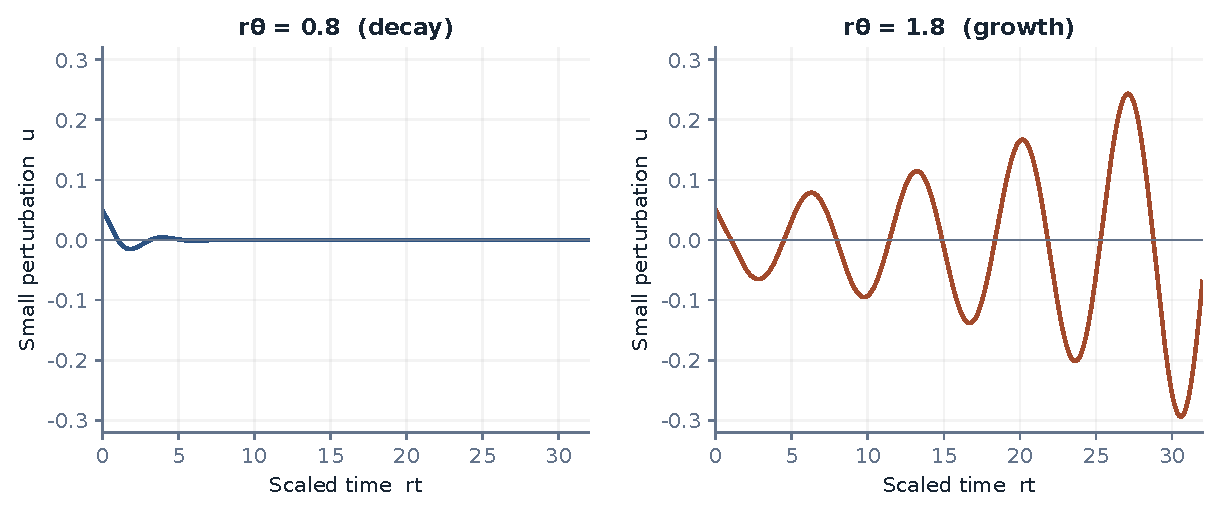
\includegraphics[width=\textwidth]{assets/delay-stability.pdf}
\caption{Linearization of the delayed logistic model near its positive equilibrium gives $\dot u=-ru(t-\theta)$. Numerical illustrations start from a small constant history. Perturbations decay at $r\theta=0.8$ and grow at $r\theta=1.8$; the first local stability boundary is $\pi/2$. These are local linear dynamics.}
\label{fig:mechanism-delay-stability}
\end{figure}
Regulated growth can settle. Delays can create oscillation. Environmental damage can reduce capacity. A richer model may need resource and waste variables as well as population.

The physical challenge is to design and maintain effective feedback before the receiving environment has changed too much. The same concern appears in ordinary manufacturing, though replication can distribute and amplify it differently.

Self-replication relocates a bottleneck toward ecological relations. It keeps the resource, time, and network questions alive.

\subsection{Consequential Weight Depends on the Task}

A reversible operation can be physically real. A draft can be deleted and still have consumed energy, time, and attention. Irreversibility therefore measures aspects of consequence; it is not a complete test for existence.

The practical question is which history remains relevant to later action. A version-controlled file can be restored. A disclosure to another person cannot be fully recalled. A simulation can reset its internal state while its user's learning persists.

The same representation can cross several boundaries. A fictional story may change a relationship. A simulated experiment may guide a real intervention. The carrier's reversibility does not settle the reversibility of its effects.

This is why a useful account specifies scale, boundary, and horizon. It asks what the project can actually recover, rather than sorting everything into “virtual” and “real.”

\subsection{The Brain in a Vat Still Needs a Plant Room}

The familiar philosophical experiment supplies a brain with artificial experience. Its epistemological question is whether the subject could distinguish the arrangement from ordinary life.

The engineering question begins outside the experience: what keeps the brain functioning?

A living brain requires a carefully maintained environment with suitable supply, waste removal, temperature, chemistry, and physiological regulation. The power level of ordinary brain metabolism is on the order of tens of watts \cite{raichle2002}. An artificial support system would have its own additional bill.

Actual perfusion and preservation research investigates parts of the problem under specific conditions. It does not establish that a conscious human brain can be maintained indefinitely outside its body. Organ preservation, temporary support, restored cellular activity, and sustained personal experience are distinct endpoints.

A simple delivery relation can show the kind of constraint involved. For one supplied substance at a time,
\begin{equation}
 \dot Q\,\Delta C\geq\dot m,
\end{equation}
where $\dot Q$ is volume flow per unit time, $\Delta C$ usable concentration difference, and $\dot m$ consumption in matching mass or molar units. A separate linear hydraulic approximation gives
\begin{equation}
 \dot Q\leq\frac{\Delta p_{\max}}{R_{\mathrm h}}.
\end{equation}
The relations illustrate a possible supply-and-pressure window. Real cerebral circulation includes regulation, changing resistance, diffusion, tissue state, and multiple substances. They are not a clinical operating formula.

Heat also needs a destination. An operating biological or computational system must remain within the conditions its substrate tolerates. Better algorithms and cooling can reduce the burden, while thermodynamics still requires an adequate heat and entropy account.

The write-in interface adds another constraint. Electrode number, coding, correlation, noise, tissue response, and long-term stability affect what signals can be delivered or read. Research on implanted interfaces documents biological responses that influence performance \cite{polikov2005response}.

For $n$ ideal independent Gaussian channels of equal bandwidth $B$, a schematic capacity is
\begin{equation}
 C(t)=nB\log_2\left(1+\frac{S}{N(t)}\right).
\end{equation}
The result is bits per second. Actual neural interfaces do not automatically satisfy the assumptions, and useful experience cannot be inferred directly from a Shannon bit rate. Noise may change over time in either direction as tissue and hardware change.

Mapping a circuit is another achievement with its own boundary. The October 2026 connectome-based fly-model preprint couples a large measured wiring graph to a simulated body and tests sensorimotor behavior \cite{minnick2026sensorimotor}. It provides a current example of wiring, dynamics, and embodied feedback being studied together. A transferred human mind would require evidence of a different order.

The distinction becomes still sharper for a proposed substitution of biological neurons with artificial components. Functional equivalence, practical replaceability, preservation of continuity, and consciousness would each need evidence or a separate argument. The engineering operation is hypothetical.

Even a successful substitution would change the substrate rather than abolish it. The new system would have some requirements for energy, temperature, communication, maintenance, and repair.

Call this \emph{substrate inescapability}: every implemented process has a material support, and the support's properties enter what the process can sustain. The claim favors no particular material.

\subsection{The Outside Remains Part of the System}

A digital environment may permit resets while its servers age, its power supply depends on a grid, and its maintenance relies on people. A biological support system may create a carefully controlled interior while shifting complexity into pumps, chemistry, redundancy, and operations.

The interior's apparent simplicity can be a real benefit. The full comparison asks whether the external support costs are lower than the alternatives and how reliably they can be carried.

The same accounting applies to ordinary remote work and automated services. Removing a commute can save real resources. A data center, network, and maintenance organization add other requirements. Counting both reveals a possible net gain rather than assuming either a miracle or an exact transfer.

The two extremes converge on a concrete conclusion. Replication can distribute construction. Simulation can reorganize experience. Each still needs a working relation with a material environment.

Locating that relation gives design more freedom. It shows which conditions can be improved, which can be delegated, and which must remain protected for the process to continue.

\section{A Method for the Next Decision}

The book began with a mismatch: proposals appear at inference speed while the world changes through many clocks. The answer is a way to inspect the route between them.

\subsection{Ask What the Capability Establishes}

A convincing interface can establish useful substitutability for a specified task. It does not settle every question about the systems behind it.

Turing's behavioral approach helped make machine intelligence an operational subject. A test's result still belongs to its test conditions. Producing an answer, maintaining a safe service, possessing a right, and bearing an obligation use different criteria.

A person's worth consequently cannot be reduced to the current scarcity of a particular output. Capabilities matter because they expand what a person and society can do. Their changing market price does not exhaust the value of a life.

Experience, relationship, participation, care, and judgment remain dimensions on which a society can choose to use its growing capacity. They need institutions and resources, rather than a promise that displaced output will automatically reappear in a higher form.

\subsection{Recalculate the Scarce Interface}

When a new tool lowers a cost, inspect what becomes scarce next.

Candidate production may give way to review. Review may improve through automatic checking and reveal a specification bottleneck. Deployment may reveal maintenance. Widely trusted service may reveal an access or distribution problem.

The movement has no fixed occupational destination. A slow activity can be improved. A trusted institution can become ceremonial. A supposedly protected skill can become easy to assess or automate.

The enduring questions concern the function. What result does this position establish? Which evidence supports it? Could another arrangement supply the same function better? Who controls access to that arrangement?

The relative importance of a function does not guarantee a good livelihood for its worker. Pay, training access, ownership, and bargaining power need their own account. Otherwise a prediction about growing care needs becomes merely a prediction about growing unpaid work.

\subsection{Three Questions Before Removing Friction}

\textbf{What does the change actually remove?} Specify the task, baseline, quality, time, and system boundary. A lower drafting time is a real gain, while a lower time to a dependable decision is a different claim.

\textbf{What happens elsewhere?} Examine review, rework, energy, infrastructure, support, exposure, and recovery. Some costs move; some fall; some appear for the first time. Measure the net result instead of assuming conservation.

\textbf{Who receives the benefit and the remaining bill?} Identify users, workers, operators, affected third parties, and future obligations. A cheaper interface can have an unequal distribution of gains even when total cost falls.

For a software team, these questions connect generation to review, regression risk, and maintenance. For a clinical service, they connect a model's measured performance to intended use, professional duties, patient rights, and follow-up. For a fleet, they connect vehicle efficiency to empty miles, coverage, infrastructure, and accident response.

The answers should be concrete enough to change the proposal. If the project discovers an overloaded review stage, it can improve selection or capacity. If a failure cannot be contained, it can narrow scope or redesign recovery. If the bill has no responsible bearer, it needs a responsibility arrangement before broad deployment.

\subsection{Keep a Few Capabilities in Practice}

At the individual level, preserve the abilities on which your own judgment depends. Let the tool handle what it does well; retain enough direct work to understand, inspect, and revise the result you rely on.

The amount differs by task. An occasional practice session can preserve one skill. Another requires continued supervised exposure. Good assistance can make both more effective.

At the organizational level, maintain the ability to reconstruct a decision. Keep proportionate records, competent reviewers, independent challenge, and usable authority to stop or correct the process.

These functions need a budget and a role. An instruction to “be careful” cannot substitute for time, access, training, and power.

Revisit retained friction too. A manual step once needed for safety may become replaceable by a better check. A learning exercise may cease to teach. Preserving the purpose requires changing the method when evidence supports change.

\subsection{Protect Choice Where Costs Are Imposed}

People affected by a decision need information and effective representation. Some can consent directly. Others require professional duties, public procedures, guardianship, or protections for interests that cannot speak for themselves.

Authority should fit competence and control, while remedies should remain usable by those carrying the loss. These are design criteria for a legitimate arrangement, not a claim that every affected person must personally operate every system.

The method can be repeated as capability grows. Identify the receiving medium. Separate the constraints. Trace the conversion into action. Examine the feedback and the bill.

A better tool changes the answers. It does not make the questions obsolete.

\section{The Negentropy Expedition}

The next machine can make an answer easier to obtain. Civilization still has to choose what to maintain, what to discover, and what costs it is prepared to impose.

The word \emph{negentropy} recalls a physical achievement: living and engineered systems can maintain local organization by using resources and exporting entropy. Its human meaning is an analogy. Thermodynamics cannot decide which organized state is worth preserving.

\subsection{Order Has a Formation Bill and a Maintenance Bill}

Copying makes the distinction visible. Let $\varepsilon_0$ be a baseline per-site error rate and $f_{\mathrm{proof}}$, $f_{\mathrm{repair}}$ illustrative residual-error factors. If their conditional effects can be combined multiplicatively,
\begin{equation}
 \varepsilon_{\mathrm{total}}
 =\varepsilon_0f_{\mathrm{proof}}f_{\mathrm{repair}},
 \qquad
 \mathbb E[M]=\varepsilon_{\mathrm{total}}L.
\end{equation}
$M$ counts errors in length $L$. Expected count and the probability of at least one error are different quantities. Copying fidelity depends on mechanism, context, dependencies, and repair \cite{kunkel2000dna}.

The calculation asks which processes preserve a usable structure across repetition. Biological proofreading, software checks, records, and institutional review do different work. Each deserves an account of cost and effectiveness.

Maxwell's demon sharpened the relation between information and physical entropy. Information can guide an action, but a complete cyclic account includes measurement, memory, and reset. Landauer's bound concerns the reset under specified physical conditions \cite{landauer1961,bennett1982thermodynamics}.

The demon is a useful warning against incomplete boundaries. A clever operation can appear free when the memory or heat sink sits outside the drawing.

The warning applies to this book's central interface. A generated proposal can be extraordinarily cheap because preparation has been amortized, the candidate is reversible, or checking happens elsewhere. Those are real technical advantages. Their value is established by the complete process they enable.

\subsection{Abundance Enlarges the Choice}

A capable civilization could use intelligence to improve health, infrastructure, education, discovery, and environmental stewardship. It could also use it to intensify competition over attention or perfect services whose goals are narrow.

The choice is not predetermined by computation. Ownership, incentives, institutions, public priorities, and individual projects influence where capacity goes.

Comfort deserves a place in that choice. Relief from pain, drudgery, exclusion, and needless delay is progress. A life also needs room for relations, curiosity, self-directed effort, and participation in something that answers back.

High-resistance frontiers supply some of those encounters. So do a difficult experiment, a maintained public service, an ecosystem patiently restored, a child educated, a relationship sustained, and a craft learned well enough to judge its tools.

They differ in scale. They share a route through consequences that cannot be established by describing the desired result alone.

\subsection{Freedom Through Better Constraints}

Freedom does not require a world without resistance. It requires usable possibilities, an understanding of relevant limits, and enough authority and support to choose among them.

Good engineering expands those possibilities. It can reduce a resource barrier, shorten a process, isolate a dependency, improve a measurement, or create a recovery path. Good institutions decide how the gains and remaining costs are shared.

The scale of intelligence makes this task more urgent. Cheap candidates increase the value of good selection. Fast action increases the value of compatible feedback. Broad reach increases the need for legitimate authority and a durable responsibility structure.

The expedition is the work of turning new possibility into a world worth sustaining. It needs powerful search, bodies and machines that can act, evidence that can interrupt a claim, and people and institutions willing to carry the long account.

Intelligence finds paths. A civilization is shaped by the paths it builds, the consequences it keeps in view, and the lives those paths make possible.

\appendix
\chapter{The Framework and Its Empirical Tests}

The main text uses mechanisms to organize the gap between proposals and dependable change. This appendix specifies how to turn that organization into a measurement program.

\section{Intellectual Lineage and Proposed Contribution}

The distinction between bits and atoms is familiar from discussions of digitization, including Negroponte's \textit{Being Digital} \cite{negroponte1995being}. This book adds life as an analytical category because adaptive, self-maintaining systems can change the pathways through which an intervention acts.

Ogburn's cultural-lag account directs attention to differing rates of technical and institutional change \cite{ogburn1922social}. Productivity debates associated with Solow direct attention to the gap between available computation and measured economic outcomes \cite{solow1987watch}. Baumol and Bowen explain how productivity differences can change relative service costs \cite{baumol1966performing,baumol1967macro}.

These traditions contain richer arguments than any short genealogy can preserve. They identify related problems without establishing one common underlying law.

The proposed contribution is a shared diagnostic language: resource barriers $R$, temporal rigidity $T$, and topological coupling $G$. The framework follows a capability through design, execution, verification, operation, and responsibility. It asks whether identifying those constraints improves explanation and decisions across domains.

The framework has three levels. A classification organizes attention. A fitted quantitative model relates operational variables to outcomes. A normative argument concerns which results, rights, and responsibilities deserve protection. Each requires its own evidence.

A useful test is comparative. Does the framework identify a bottleneck earlier, improve prediction, reveal an omitted cost, or distinguish interventions that a simpler account treats alike? The value of the language lies in those gains.

\section{Three Mathematical Forms}

\subsection{An Exponential Cost Model}

First choose an outcome. Let $C>0$ denote cost, labor, or mean time per acceptable result for a fixed task and boundary. Choose a matching reference $C_{\mathrm{ref}}>0$, and define a dimensionless response $\eta=C/C_{\mathrm{ref}}$.

If the marginal effects of normalized constraints on log cost are approximately constant, an initial model is
\begin{equation}
 \eta=\eta_0\exp(\alpha R+\beta T+\gamma G).
\end{equation}
$R,T,G$ are dimensionless measurements whose definitions and baselines must be published. The coefficients describe log-cost changes per unit of those measurements. Positive signs are hypotheses for the chosen definitions.

The additive exponent gives multiplicative relative-cost factors. It does not follow merely because stages are connected in series. Serial durations can add, parallel completion can depend on a maximum, and steady pipeline capacity can depend on a bottleneck.

With constant coefficients, fixed $G$ and baseline, and $\alpha\neq0$, an equal-cost slope is
\begin{equation}
 \left(\frac{\partial R}{\partial T}\right)_\eta
 =-\frac{\beta}{\alpha}.
\end{equation}
This is a slope in the assumed response surface. It does not show that the project has an available intervention following that direction.

Interactions can be tested by adding terms such as $\delta RT$. Threshold, saturating, additive-cost, and nonparametric alternatives should be compared. An exponential has a smoothly increasing marginal cost; it does not by itself create a phase transition or critical threshold.

Variables must be constructed independently enough to avoid circularity. Relabeling observed completion time as “temporal rigidity” and then using it to predict completion time supplies little explanation.

Estimate on one sample, check later periods and comparable projects, and inspect residuals by task and medium. Structured residuals may reveal missing variables or a wrong form. Unstructured residuals in a small sample do not establish a mechanism.

Coefficient drift can reflect changing technology, omitted conditions, or unstable definitions. It does not by itself prove reversed causality. Record which interpretation the available evidence can distinguish.

\subsection{A Timescale Ratio}

The Deborah number compares relaxation and observation or driving timescales \cite{reiner1964deborah}:
\begin{equation}
 \mathrm{De}=\frac{\tau_{\mathrm{relax}}}
                  {\tau_{\mathrm{obs}}}.
\end{equation}
Specify the mechanism. A system can have many relaxation times: equipment replacement, workforce training, inventory adjustment, and rule revision need not share a value.

In a material model, a small ratio means substantial relaxation within the chosen timescale; a large ratio means the material retains more of its unrelaxed response. Social applications require evidence for an analogous adjustment mechanism.

Changing the observation window changes the description, not the system's actual recovery capacity. Governance changes a mismatch by changing the input, response capability, coupling, or buffer.

If a single-time Maxwell material is an appropriate physical model, its loss modulus peaks near $\omega\tau=1$. A social adjustment process does not acquire the same peak simply because a timescale ratio has been assigned to it.

\subsection{A Rate-Dependent Resistance}

Over a defined thickening range, a simple rheological form is
\begin{equation}
 \eta(\dot\gamma)=\eta_b+k\dot\gamma^n,
 \qquad k>0,\quad n>0.
\end{equation}
For dynamic viscosity in $\mathrm{Pa\,s}$ and shear rate in $\mathrm{s^{-1}}$, $k$ has units $\mathrm{Pa\,s^{n+1}}$. The expression supplies a rising branch, not a universal complete flow curve.

Biological and institutional applications must define intervention rate and effective resistance in their own units. Dose, frequency, cumulative exposure, and pace are different variables. Compensation, damage, adaptation, and recovery can generate several response shapes.

To test a power law, measure a sufficiently wide input range, repeat the measurements, and compare threshold and saturation models. With a non-negligible baseline $\eta_b$, the slope of $\ln\eta$ against $\ln\dot\gamma$ is not identically $n$. Either fit the full expression or justify a range in which the baseline can be neglected.

The physical model and its cross-domain application occupy different evidential positions. A familiar curve suggests a candidate mechanism; measurements in the target system decide whether it belongs there.

\section{Qualitative Use Before Calibration}

The framework can guide investigation before its coefficients are known. Classify constraints using public criteria and record the evidence supporting each classification.

\subsection{Eight Regions}

For a coarse view, mark each coordinate low or high under a declared scale. The three binary classifications yield eight regions.

\begin{table}[ht]
\centering\small
\begin{tabularx}{\textwidth}{@{}cccYY@{}}
\toprule
$R$ & $T$ & $G$ & Initial focus & Questions to investigate\\
\midrule
Low & Low & Low & The remaining service boundary & Is demand, quality, or an omitted constraint limiting use?\\
High & Low & Low & Resource barrier & Can substitution, efficiency, or scale improve access?\\
Low & High & Low & Time & Which waiting periods supply information or complete a process?\\
Low & Low & High & Coupling & Can interfaces or dependencies be isolated?\\
High & High & Low & Resources and time & Which stages can be redesigned or parallelized?\\
High & Low & High & Resources and coupling & Can a different architecture reduce both?\\
Low & High & High & Time and coupling & Which interacting responses determine the schedule?\\
High & High & High & The full conversion chain & What phased or alternative route is feasible?\\
\bottomrule
\end{tabularx}
\caption{Regions identify an investigation priority. They do not rank total cost or predict a launch date.}
\end{table}

Near a classification boundary, report the neighboring categories and the evidence that could distinguish them. The cost of coarse classification is loss of within-category detail.

\subsection{Comparison Without a Full Weight Vector}

For comparable states under the exponential model,
\begin{equation}
 \ln\frac{\eta_a}{\eta_b}
 =\alpha\Delta R+\beta\Delta T+\gamma\Delta G.
\end{equation}
With positive coefficients and matching scales, a state no higher on any constraint and lower on at least one has a lower modeled response. This dominance relation does not require exact weights.

Mixed changes need more information. A reduction in $R$ and an increase in $G$ cannot be ranked from their signs alone. Coefficient ratios, magnitudes, and uncertainty bounds determine the result.

Ordinal grades support within-coordinate order. They do not establish equal intervals or a common scale across coordinates. Grade “four” in resources cannot be compared directly with grade “three” in time.

\subsection{Direction Over Time}

With fixed baseline and coefficients,
\begin{equation}
 \frac{\mathrm d\ln\eta}{\mathrm dt}
 =\alpha\dot R+\beta\dot T+\gamma\dot G.
\end{equation}
Common-direction changes permit a sign judgment under positive weights. Mixed directions require bounds or estimates. If coefficients and baseline change, their derivative terms must be included.

This is enough to organize some useful questions: is the physical constraint falling while review remains unchanged? Does a new interface reduce resource use but expand dependencies? Is a reported gain a change in the task boundary?

The qualitative account should end with evidence needs. It can identify an unresolved tradeoff without inventing a numerical answer.

\section{Decomposition and a Usable Rating Sheet}

A rating sheet makes a diagnosis inspectable. Its purpose is to connect each assessment with a task, boundary, and piece of evidence.

\subsection{Choose Units That Can Be Examined}

A unit should have an output that can be checked and an internally coherent process. Large differences in response time can signal a need to split it. A starting heuristic is
\begin{equation}
 \frac{\max_j\tau_j}{\min_j\tau_j}\leq\Lambda,
\end{equation}
with a declared $\Lambda$, perhaps ten. This does not guarantee that another subdivision is useless. The chosen grain must still preserve the mechanism being investigated.

Distinguish conversion units from interface units. A manufacturing step produces an item for the next step. Certification, procurement, access, and public participation connect the project to other systems. Both can change through better technology and organization.

\subsection{Ordinal Anchors}

The following anchors describe increasing constraint. They require task-specific criteria and evidence; they do not assign universal powers of ten.

\begin{table}[ht]
\centering\small
\begin{tabularx}{\textwidth}{@{}cYYY@{}}
\toprule
Grade & Resources & Time & Coupling\\
\midrule
0 & Small marginal demand within existing capacity & Effectively immediate for the task & Local change with few dependencies\\
1 & Available general equipment and supply & Short relative to the operating cycle & Known, standardized interfaces\\
2 & Dedicated equipment or materials & A material part of an operating cycle & Several interfaces need adaptation\\
3 & Significant supply, capital, or infrastructure commitments & A substantial planning or build cycle & Multiple teams or suppliers must coordinate\\
4 & Scarce inputs or major capacity changes & Long observation, replacement, or institutional process & Multiple organizations or jurisdictions interact\\
5 & A severe constraint under the specified boundary & Very long relative to the decision horizon & Extensive dependencies with difficult isolation\\
\bottomrule
\end{tabularx}
\caption{Illustrative ordinal anchors. A grade is an evidence-backed category, not a calibrated physical quantity.}
\end{table}

Grade zero still consumes material resources. Grade five does not establish impossibility. A physical conservation law can constrain a task without proving that every possible design has reached its limit.

Record uncertainty as an interval of plausible grades or a statement of missing evidence. A decimal grade creates no precision unless the scale has been calibrated.

For a defined dependency closure size $d_i$, one optional count-based binning is
\begin{equation}
 G_i=\min\left\{5,\left\lfloor\log_{10}(1+d_i)\right\rfloor\right\}.
\end{equation}
The closure definition matters more than the bin. Graph reachability, mandatory simultaneous modification, causal influence, and administrative contact are different relationships.

\subsection{Aggregate the Quantities Before the Grades}

Resources with matching units and boundaries can be added. Electricity, labor, cash, and materials need separate accounts or an explicit conversion. Averaging ordinal resource grades does not reconstruct total resource use.

Time depends on structure. For a serial chain with durations $t_i$,
\begin{equation}
 t_{\mathrm{serial}}=\sum_i t_i.
\end{equation}
For simultaneous tasks required before completion, elapsed time is their maximum. For a dependency graph it is the longest feasible path, under the stated resource and scheduling assumptions:
\begin{equation}
 t_{\mathrm{finish}}
 =\max_{p\in\mathcal P}\sum_{i\in p}t_i.
\end{equation}
A steady pipeline's throughput can be limited by its slowest stage. Throughput and first-item completion time are different quantities.

Amdahl's law supplies another conditional bound:
\begin{equation}
 S(n)=\frac{1}{s+(1-s)/n}\longrightarrow\frac1s,
 \qquad s\in(0,1].
\end{equation}
It assumes a fixed workload, serial fraction $s$, ideal parallelization of the remaining part, and omitted additional overhead \cite{amdahl1967validity}. An algorithm change can alter the workload or serial fraction.

Coupling needs a graph account. Report relevant degree and closure distributions, shared dependencies, cut sets, critical nodes, and possible cascade routes. A mean of coupling grades can conceal a decisive hub.

The familiar giant-component condition
\begin{equation}
 \frac{\langle k^2\rangle}{\langle k\rangle}>2
\end{equation}
belongs to a specified asymptotic random-graph setting with suitable regularity assumptions \cite{molloy1995critical}. It is not a universal threshold for directed, clustered, weighted industrial dependency networks. A connected component also does not imply simultaneous mandatory change.

Only after operational quantities have been defined and calibrated should they enter a quantitative model. A grade sheet remains useful without that step.

\subsection{What to Improve First}

Under a calibrated exponential model, the contribution $\alpha_c c$ can identify a large modeled constraint term. Choosing an intervention also needs the feasible reduction, cost, interactions, and risk.

For a small independent change with cost per unit reduction $\mu_c>0$, the ratio $\alpha_c/\mu_c$ compares modeled marginal log-cost benefit per spending unit. It does not establish absolute net benefit or select the best finite project when interventions interact.

If time is explicitly calibrated as $T=\log_{10}(\tau/\tau_0)$, then
\begin{equation}
 \ln\mathrm{De}=(\ln10)T
 -\ln\frac{\tau_{\mathrm{drive}}}{\tau_0}.
\end{equation}
This identity follows from that calibration. It cannot be inferred from a qualitative time grade.

\subsection{Worked Audit: A Low-Altitude Service}

Split a proposed service into cell production, pack and thermal system, airframe and rotors, flight control, terminals, operations and maintenance, airworthiness, airspace access, and the conditions under which the public will accept the service.

For each unit, collect actual durations, resource requirements, dependencies, validation evidence, and a responsible party. “Public acceptance takes ten years” is not an input one may simply declare. Identify the relevant population, decision, and observable acceptance condition.

A flight-control update can require substantial verification even when code changes quickly. Certification uses people, equipment, tests, and facilities. Airspace coordination uses infrastructure and operations. None is physically free because its output is a permission.

Create the dependency graph, then distinguish stages that run concurrently from those waiting on one another. A better battery may change aircraft performance, reserves, economics, and certification evidence together. The effect on launch time depends on the actual critical path.

If the next required authorization remains on that path, shortening an unrelated manufacturing step may not move the launch date. It can still reduce cost or improve later throughput. The method separates those outcomes.

\subsection{Five Comparison Questions}

\begin{table}[ht]
\centering\small
\begin{tabularx}{\textwidth}{@{}lYY@{}}
\toprule
Project & Resource and time questions & Dependency and evidence questions\\
\midrule
Inference service & Which capacity exists, and what does the whole request cost? & Which downstream actions can an output trigger?\\
Advanced fabrication & Which equipment, process, and yield constraints bind? & Which process changes need supplier and validation changes?\\
Low-altitude service & What mission energy, reserves, and facilities are required? & What evidence and authorizations govern the actual operation?\\
Gene-editing therapy & What delivery, production, exposure, and follow-up are required? & Which cell populations and clinical outcomes support the intended use?\\
Cement or steel decarbonization & What route, energy, feedstock, and replacement schedule are feasible? & How do plant, power, transport, product standards, and demand interact?\\
\bottomrule
\end{tabularx}
\caption{Comparable questions replace unsupported universal sector scores.}
\end{table}

The report should let another reader change an assessment by pointing to evidence. That is the rating sheet's central promise.

\begin{figure}[ht]
\centering
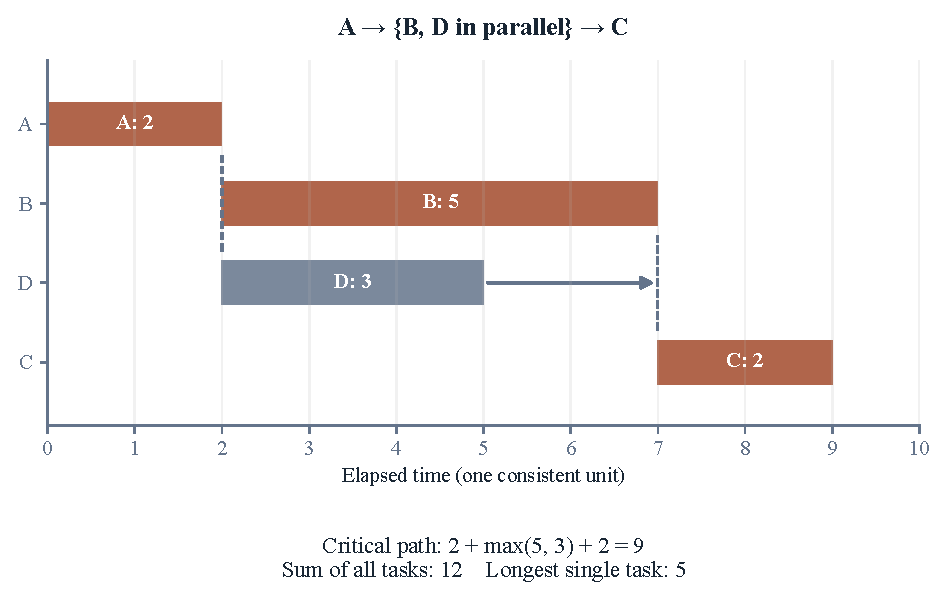
\includegraphics[width=\textwidth]{assets/critical-path.pdf}
\caption{A precedes parallel tasks B and D; C waits for both. Completion takes $2+\max(5,3)+2=9$, rather than the sum of all tasks (12) or the longest individual task (5). The critical path is A--B--C.}
\label{fig:mechanism-critical-path}
\end{figure}

\section{Three Response Models and Their Tests}

The medium suggests mechanisms to investigate. The task and data determine which response model fits.

\subsection{Approach to a Usage Plateau}

For a defined digital service under sufficiently stable conditions, an illustrative model is
\begin{equation}
 Y_{\mathrm{bits}}(t)=Y_\infty(1-e^{-t/\tau}).
\end{equation}
The initial value is zero. The response approaches a fitted plateau $Y_\infty$ over timescale $\tau$. Demand, budgets, distribution, usefulness, and capacity can all affect the parameters.

Measure actual use or effective service, not merely generated volume. Compare the exponential approach with alternatives and re-estimate after material changes in the environment.

\subsection{A Capacity-Limited Physical Process}

For fixed facilities and a consistently defined input $I$, one possible model class satisfies
\begin{equation}
 0\leq Y_{\mathrm{atoms}}(I)\leq\Phi_{\max}.
\end{equation}
If diminishing marginal gains are additionally proposed over the observed range,
\begin{equation}
 \frac{\partial^2Y_{\mathrm{atoms}}}{\partial I^2}\leq0.
\end{equation}
The upper bound and concavity are separate assumptions. New capacity, learning, complementarities, or step changes can violate the latter and change the former.

Measure design, fabrication, construction, verification, and maintenance separately. AI can improve one stage without determining the rest. Complete-task measurements are needed before comparing its effect across industries.

\subsection{An Adaptive Response}

For one specified biological or adaptive process, a candidate observation is
\begin{equation}
 \frac{\mathrm d\langle Y\rangle}{\mathrm dP}\approx0,
 \qquad
 \frac{\mathrm d\,\operatorname{Var}(Y)}{\mathrm dP}>0,
 \quad P>P_c.
\end{equation}
Mean benefit reaches a plateau while dispersion increases beyond a fitted threshold. Other processes can improve, decline, or respond after a delay. A variance increase is not automatically an increase in harmful outcomes; the outcome definition must identify the risk.

Collect input intensity, duration, population, baseline state, repeated measurements, and follow-up. Distinguish dose from pace. Experiments or credible comparison designs must separate the intervention's effect from selection and changing conditions.

\subsection{A Common Evaluation Record}

The three examples use different independent variables: time, input, and intervention intensity. Their plotted slopes are not directly comparable.

To compare a shared technology across stages or media, fix a useful task, define comparable input and outcome measures, and record the resources, elapsed time, accepted results, failures, and maintenance required. Matched projects, staged deployments, and suitable experimental designs can then test particular mechanisms.

A multistage project's total output is generally not a linear sum of these three curves. Interactions and bottlenecks require a model of the actual chain.

The empirical program succeeds when it identifies which constraint changed, what happened downstream, and whether a competing explanation accounts for the same evidence more simply.

\section{Standards of Evidence}

The classification, mathematical forms, and normative claims should be assessed separately.

A classification earns its place by helping identify mechanisms or distinguish cases. A quantitative model needs defined variables, stable boundaries, calibrated parameters, and out-of-sample evaluation. A normative proposal needs public reasons about interests, rights, authority, and distribution.

Physical terms require a demonstrated correspondence when applied elsewhere. A biological thickening model needs an input, a response, and a mechanism. A social Deborah number needs an identifiable adjustment process and timescale. Similar language or curve shape supplies a hypothesis to investigate.

The exponential form should compete with interaction, threshold, saturation, and simpler alternatives. If adequate fit requires repeatedly changing what the coordinates mean, revisit the definitions. If several media show the same curve, inspect the mechanism before deciding what the similarity implies.

The framework's central practical claim is that proposals become dependable changes through a chain with receiving capacities, feedback, and obligations. Its usefulness can be tested by whether following that chain improves decisions.

The book's normative commitments are explicit: affected people need effective participation and remedies; consequential judgments need evidence; authority needs an accountable scope; and progress should be assessed over the relevant system and time.

Application begins with feasible paths and a full account of cost. It then considers the interests and rights involved, establishes authority and responsibility, and preserves records through which the result can continue to be challenged and improved.

\printbibliography[title={References}]
\end{document}
